\part{De Freud aos debates atuais:\\ psicanálise e feminismo}


\chapter*{Introdução a \emph{Feminine sexuality}\footnote{Traduzido
  do inglês por João Cunha e Léa Silveira. Este texto corresponde à
  segunda introdução do volume \emph{Feminine sexuality -- Jacques Lacan
  and the école freudienne}, editado por Juliet Mitchell e
  Jacqueline Rose, e traduzido por esta (The Macmillan Press \versal{LTD}, 1982).
  {[}\versal{N.~T.}{]}}}
\addcontentsline{toc}{chapter}{Introdução a \emph{Feminine sexuality}, \footnotesize\emph{por Jacqueline Rose}}
\hedramarkboth{Introdução a \emph{Feminine sexuality}}{}

\begin{flushright}
\emph{Jacqueline Rose}
\end{flushright}

%\begin{quote}
\epigraph{Freud adianta que só há libido masculina. O que quer dizer isso? ---
senão que um campo, que nem por isso é coisa alguma, se acha assim
ignorado. Esse campo é o de todos os seres que assumem o estatuto da
mulher --- se é que esse ser assume o que quer que seja por sua conta.}{(Lacan, \emph{Encore}, \versal{SXX}, 1972-3)}
%\end{quote}

Os textos que publicamos aqui\footnote{Ver nota 1. {[}\versal{N.~T.}{]}} retornam
ao debate já descrito,\footnote{Por Juliet Mitchell, na primeira
  introdução ao volume mencionado. {[}\versal{N.~T.}{]}} ampliando"-o. Eles
retornam ao debate para insistir que suas implicações para a psicanálise
ainda não foram compreendidas; eles o ampliam na medida em que o próprio
tema --- da sexualidade feminina --- extravasa da psicanálise para o
feminismo, como parte de seu questionamento acerca de como a sexualidade
pode ser definida.

Nesse sentido, estes textos carregam todos os sinais de uma repetição,
de um ressurgimento de uma área de desacordo e perturbação; uma área na
qual, porém, o tema em questão foi lançado em vista de conferir ao
debate um acentuado relevo. É como se a coexistência, mais ou menos
pacífica que encerrou o debate nos anos 1920 e 1930 (``deixada, num
entendimento tácito, à boa vontade da interpretação individual'',
\versal{C},\footnote{Quando as traduções dos trechos que são citados tiverem sido
  feitas pela própria Rose, optaremos por seguir a autora e fazer uma
  tradução de sua tradução, checando o resultado com o texto original.
  Operamos aqui com o entendimento de privilegiar o argumento de Rose,
  tentando acompanhar o mais próximo possível as opções de linguagem
  feitas pela autora. Quando ela recorrer a versões de outros tradutores
  e a obra em questão estiver disponível em português, usaremos a versão
  brasileira; em todos os casos, as versões em inglês, usadas por Rose,
  estarão indicadas na bibliografia final. As abreviaturas empregadas
  referem"-se aos seguintes textos, publicados em \emph{Feminine
  sexuality}: \versal{C} -- \emph{Guiding remarks for a congress on feminine
  sexuality;} \versal{MP} -- \emph{The meaning of the phallus}; \versal{PP} -- \emph{The
  phallic phase and the subjective import of the castration complex};
  \versal{IT} -- \emph{Intervention on transference}; \versal{FS} -- \emph{Feminine
  sexuality in psychianalytic doctrine}; \versal{E} -- \emph{God and the}
  jouissance \emph{of The Woman}/\emph{A love letter} (em
  \emph{Encore}); \versal{O} -- \emph{Seminar of 21 January 1975.} {[}\versal{N.~T.}{]}}
pp. 88-9), e a calmaria produzida (``calmaria experenciada após a pane
do debate'', \versal{C}, p. 89), tivesse escondido um problema que
inevitavelmente voltaria a emergir com renovada urgência. Hoje, essa
urgência pode ser vista explicitamente como política, tanto é que, na
controvérsia a respeito da dissolução, feita por Lacan, de sua escola em
1980, o jornal francês \emph{Le Monde} indicava o debate sobre
feminilidade como a declaração mais evidente das repercussões políticas
da própria psicanálise (\emph{Le Monde}, primeiro de junho de 1980, p.
xvi). A psicanálise é agora reconhecida como crucial na discussão da
feminilidade --- a discussão a respeito de como ela surge e o que isso
pode significar. Jacques Lacan, que abordou cada vez mais essa questão
no curso de seu trabalho, tem estado no centro das disputas provocadas
por tal reconhecimento.

Nesse contexto, a ideia de um ``retorno a Freud'', frequentemente
associada a Lacan, tem um significado muito específico. Tem pouco a ver
com um retorno à letra do texto de Freud, como se se tratasse da
reabertura de um caso, um caso que já teria sido disputado, tal como
Juliet Mitchell descreve acima, e acerca do qual se poderia dizer que
Freud, com relação ao feminismo, teria saído perdendo. De fato, a
relação entre psicanálise e feminismo pode parecer começar no momento em
que a abordagem de Freud sobre a diferença sexual foi rejeitada por
analistas que argumentavam \emph{em favor} das mulheres (``analistas
homens foram levados a adotar uma visão excessivamente falocêntrica'',
Jones, 1927, p. 459). Desde então, a maioria dos analistas concordam com
as limitações e dificuldades da argumentação de Freud. Tais dificuldades
foram inteiramente reconhecidas por Lacan, mas ele considerou que as
tentativas de resolvê"-las no contexto da psicanálise sistematicamente
caem numa armadilha. Pois elas fracassaram em ver que o conceito de falo
na argumentação de Freud sobre a sexualidade humana fazia parte da sua
lucidez quanto ao caráter problemático, ou mesmo impossível, da própria
identidade sexual. Responderam"-lhe recorrendo a um dado prévio à
diferença sexual com o intuito de assegurar essa identidade para ambos
os sexos. Assim procedendo, tais respostas perderam de vista o fato de
que, em Freud, a diferença sexual é construída ao preço de envolver a
sujeição a uma lei que ultrapassa qualquer divisão natural ou biológica.
O conceito de falo representa essa sujeição e a maneira pela qual as
mulheres estão implicadas de um modo muito preciso nesse processo.

A história da psicanálise, sob diversos aspectos, pode ser vista
inteiramente a partir das maneiras pelas quais se processou o
engajamento com a questão da sexualidade feminina. O próprio Freud
começou com a análise da histeria (Freud e Breuer, \versal{II}, 1893-5) --- e
insistiu, cabe destacar, no fato de que o paciente histérico poderia
também ser um homem (Freud, \versal{I}, 1886). Foi seu fracasso em analisar uma
paciente histérica --- ``Dora'' (Freud, \versal{VII}, 1905) ---, em termos de um
conceito normativo daquilo que uma mulher poderia ser ou querer, que o
levou a admitir a natureza fragmentada e aberrante da própria
sexualidade. A sexualidade normal é, desde então, estritamente um
\emph{ordenamento} que o histérico recusa (adoecendo). O restante da
obra de Freud pode, então, ser lido nos termos de uma descrição de como
esse ordenamento vem a se colocar, o que o levou, necessariamente, de
volta para a questão da feminilidade, porque sua persistência como
dificuldade revelou o custo desta ordem.

Além disso, Freud retomou essa questão no momento em que estava
reformulando sua teoria da subjetividade humana. Lacan tomou o conceito
freudiano de inconsciente, ampliado e desenvolvido nos textos
posteriores (especificamente, \emph{Além do princípio do prazer}, \versal{XVIII},
1920, e o ensaio inacabado \emph{Divisão do Eu no processo de defesa},
\versal{XVIII}, 1940) como base de sua própria explicação da feminilidade (aqui,
a frequente crítica a Lacan segundo a qual ele não teria levado em conta
os textos tardios de Freud é totalmente infundada). Ele argumentou que a
incapacidade em reconhecer a interdependência entre essas duas
preocupações na obra de Freud --- a teoria da subjetividade e da
feminilidade, juntas --- levou os psicanalistas a um grave erro
ideológico, ou seja, aquele de tentar resolver as dificuldades da
argumentação freudiana sobre a feminilidade pretendendo resolver a
dificuldade da própria feminilidade. Pois, ao reconduzirem a mulher a
seu lugar e a sua identidade (algo que, segundo eles, Freud não teria
visto em virtude de seus ``preconceitos''), eles perderam a ênfase
correlata de Freud na divisão e na precariedade da própria subjetividade
humana; a qual, para Lacan, foi central para os \emph{insights} mais
radicais da psicanálise. Tentativas de responder a Freud por parte de
mulheres e para as mulheres tenderam a renunciar a estes
\emph{insights}, seja descartando o conceito de inconsciente (o sinal
dessa divisão), seja a bissexualidade (o sinal dessa precariedade). E
isso vale para posições tão diversas quanto as de Jones (e Horney) nos
anos 1920 e 1930, e a de Nancy Chodorow (1979)\footnote{Ver nota 10,
  abaixo.} ao falar de psicanálise para o feminismo hoje.

A retomada do debate sobre sexualidade feminina deve começar, então,
pela ligação entre sexualidade e inconsciente. Nenhuma explicação da
obra de Lacan que pretenda separar esses dois aspectos pode fazer
sentido. Para Lacan, o inconsciente desautoriza o sujeito de qualquer
posição de certeza, de qualquer relação de saber a respeito de sua
história e de seus processos psíquicos; e, \emph{simultaneamente},
revela a natureza ficcional da categoria sexual à qual, mesmo assim,
todo sujeito é destinado. Segundo Lacan, a identidade sexual funciona
como uma lei --- trata"-se de algo imposto ao sujeito. Para ele, o fato de
que os indivíduos devem se alinhar segundo uma oposição (ter ou não
falo) torna isso claro. Mas é a constante dificuldade, ou mesmo
impossibilidade, desse processo que é enfatizada por Lacan; e é a isso
que cada um dos textos desta coletânea se reporta de diferentes modos.
As exposições dessa dificuldade na psicanálise e para o feminismo são,
pois, partes de um mesmo projeto.

\section{I}

A ligação entre sexualidade e inconsciente foi constantemente enfatizada
por Lacan: ``não omitamos o que é, em primeiro lugar, sublinhado por
Freud como estritamente consubstancial à dimensão do inconsciente''
(\versal{SXI}, p. 133, \emph{p. 146, p. 139}).\footnote{Na sequência: página da
  edição francesa, da inglesa e da brasileira. {[}\versal{N.~T.}{]}} Outras
interpretações, como a de Ernest Jones, descreveram a aquisição da
identidade sexual como desenvolvimento do ego e/ou maturação de pulsões.
Lacan considerou que todos esses conceitos se esteiam no mito de uma
coesão subjetiva que, propriamente, o inconsciente subverte. Para Lacan,
a descrição da sexualidade em termos desenvolvimentistas invariavelmente
perde de vista a descoberta mais fundamental de Freud --- que o
inconsciente nunca cessa de desafiar nossa aparente identidade como
sujeitos.

A abordagem lacaniana da subjetividade sempre foi desenvolvida em
referência à ideia de uma ficção. Assim, na década de 1930, ele
introduziu o conceito de ``estádio do espelho'' (\emph{Ecrits}, (1936)),
tomando a imagem da criança no espelho como modelo e base para suas
futuras identificações. Essa imagem é uma ficção porque esconde, ou
congela, a falta de coordenação motora do infante e a fragmentação de
suas pulsões. Mas ela é salutar para a criança, pois lhe fornece o
primeiro sentido de uma identidade coerente na qual possa reconhecer a
si mesma. Para Lacan, no entanto, isso já é uma fantasia --- a mesma
imagem que situa a criança também divide sua identidade em duas. Além
disso, esse momento só tem sentido em relação à presença e ao olhar da
mãe, que garante sua realidade para a criança. A mãe não (como na
argumentação de D. W. Winnicott (Winnicott, 1967)) espelha a criança
para si mesma; ela outorga uma imagem \emph{para} a criança, que sua
presença instantaneamente desvia. O ato de segurar a criança deve, pois,
ser entendido não apenas como um processo de contenção, mas como um
processo de referência, que fratura a unidade que ele parece oferecer. A
imagem no espelho é central na abordagem lacaniana da subjetividade,
pois suas aparentes suavidade e totalidade são tomadas como um mito. A
imagem pela qual reconhecemos a nós mesmos pela primeira vez corresponde
a um \emph{falso reconhecimento}. Lacan tem o cuidado de enfatizar,
porém, que seu ponto de vista não se restringe apenas ao campo do
visível: ``a ideia do espelho deve ser entendida como um objeto que
reflete --- não apenas o visível, mas também o que é ouvido, tocado e
querido pela criança'' (Lacan, 1949, p. 567).

Então, Lacan toma a imagem no espelho como modelo da própria função do
ego, a categoria que permite ao sujeito operar como ``eu''. Ele apoia
seu argumento na linguística, que designa o pronome como um
``\emph{shifter}'' (Benveniste, 1956). O ``eu'' com o qual falamos
representa nossa identidade como sujeitos na linguagem, mas é a entidade
menos estável na linguagem, uma vez que seu sentido se coloca puramente
em uma função do momento de enunciação. O ``eu'' pode sofrer
deslocamento {[}\emph{shift}{]}, mudar de lugar, pois apenas e sempre se
refere a quem o estiver empregando naquele momento.

Para Lacan, o sujeito é constituído através da linguagem --- a imagem no
espelho representa o momento no qual o sujeito é localizado numa ordem
que lhe é alheia e à qual ele se referirá daí por diante. O sujeito é o
sujeito \emph{da} fala (o ``\emph{parle"-être}'' de Lacan) e sujeito
\emph{a} essa ordem. Mas, se há divisão na imagem, e instabilidade no
pronome, há igualmente perda e dificuldade na palavra. A linguagem só
pode operar designando um objeto em sua ausência. Lacan leva isso mais
longe e afirma que a simbolização verte o objeto \emph{como} ausência.
Ele oferece como sua referência a primeira explicação de Freud sobre a
catexia alucinatória da criança no objeto pelo qual ela chora (Freud, \versal{I},
1895, p. 319) e sua descrição posterior, em \emph{Além do princípio do
prazer} (Freud, xviii, 1920, p. 14), da simbolização que a criança faz
da ausência da mãe quando brinca. No primeiro exemplo, a criança alucina
o objeto que deseja; no segundo, ela joga um carretel de linha para fora
de seu berço a fim de simbolizar a ausência e a presença da mãe. A
simbolização começa, portanto, quando a criança começa a perceber que
algo pode estar ausente; palavras representam objetos porque elas só
precisam ser faladas a partir do momento em que o primeiro objeto é
perdido. Para Lacan, o sujeito só pode operar na linguagem repetindo
constantemente esse momento de divisão fundamental e irredutível. O
sujeito é, pois, constituído na linguagem \emph{como} esta divisão, como
esta cisão (\emph{Ichspaltung}, ou cisão do ego, é o termo de Freud).

Lacan denominou ``simbólico'' a ordem da linguagem e ``imaginário'' a do
ego e de suas identificações (a ênfase, portanto, está deliberadamente
no símbolo e na imagem, a ideia de algo que ``está no lugar de''). O
``real'' foi, então, seu termo para expressar o momento de
impossibilidade no qual ambos estão inseridos, o ponto eterno de retorno
àquele momento.\footnote{Isso pode ser comparado, por exemplo, com a
  descrição que Melanie Klein faz da formação de símbolos (Klein, 1930)
  e também com aquela de Hannah Segal (1957); nelas a simbolização é um
  efeito de ansiedade e um meio de transcendê"-la na direção da
  realidade, direção cada vez mais assegurada pelo fortalecimento do
  próprio ego. Cf. também a crítica específica de Lacan ao famoso artigo
  de Ernest Jones sobre simbolismo (Jones, 1916; \emph{Ecrits} (1959)),
  que ele criticou tendo em vista a definição de linguagem em termos de
  um domínio ou apropriação crescente da realidade e por ter, por
  conseguinte, fracassado em alcançar a estrutura da metáfora (ou
  substituição) que reside na raiz da subjetividade, sendo infinitamente
  repetida nela, em sua relação com o inconsciente. É nesse sentido
  também que a ênfase de Lacan na linguagem deve ser diferenciada do que
  ele definiu como ``culturalismo'', isto é, de qualquer concepção da
  linguagem como um fenômeno social que não leve em conta sua
  instabilidade fundamental (linguagem como um algo que constantemente
  põe e \emph{desloca} o sujeito).}

A concepção lacaniana da infância segue, então, a premissa básica de que
a identidade é construída na linguagem, mas somente a um custo. A
identidade altera"-se e a linguagem fala da perda que subjaz àquele
primeiro momento de simbolização. Quando a criança pede alguma coisa
para sua mãe, essa perda persistirá através de qualquer coisa que ela
eventualmente ofereça, ou diga, como resposta. A demanda sempre
``carrega algo distinto daquilo que é requerido pela satisfação'' (\versal{MP},
p. 80) e cada vez que a demanda da criança é respondida com a satisfação
de suas necessidades, então essa ``outra coisa'' é relegada ao lugar de
sua impossibilidade original. Lacan designa isso ``desejo''. O que pode
ser definido como o ``resto'' do sujeito, algo que sempre é deixado de
lado, mas que, como tal, não tem conteúdo. O desejo funciona da mesma
forma que a unidade zero na cadeia numérica --- seu lugar é, ao mesmo
tempo, constitutivo \emph{e} vazio.

O conceito de desejo é crucial para a abordagem lacaniana da
sexualidade. Lacan considerou que a falta de compreensão de suas
implicações conduz novamente, de modo inevitável, a uma redução da
sexualidade à ordem da necessidade (algo que, portanto, poderia ser
satisfeito). Contra isso, ele citou a afirmação de Freud: ``(\ldots{})
devemos considerar a possibilidade de que alguma coisa na natureza da
própria pulsão sexual não seja favorável à realização da plena
satisfação'' (Freud, \versal{XI}, 1912, pp. 188-9, 149; cit. \versal{PP}\footnote{O texto
  referido por esta abreviatura --- \emph{The phallic phase and the
  subjective import of the castration complex} --- não é de autoria de
  Lacan, tendo sido publicado anonimamente em \emph{Scilicet}. Cf.
  \emph{Feminine sexuality}, \emph{op. cit.}, p.~99. {[}\versal{N.~T.}{]}} p.
113).

Ao mesmo tempo, ``identidade'' e ``totalidade'' permanecem,
precisamente, no nível da fantasia. Sujeitos na linguagem persistem em
sua crença de que em algum lugar há um ponto de certeza, de saber e de
verdade. Quando o sujeito endereça sua demanda para fora de si próprio
no outro, este outro se torna exatamente o lugar fantasiado desse saber
ou certeza. Lacan chama isso de o Outro --- o lugar da linguagem ao qual
o sujeito falante necessariamente se refere. O Outro parece manter a
``verdade'' do sujeito e o poder de compensar sua perda. Mas essa é a
fantasia final. A linguagem é o lugar em que o sentido circula --- o
sentido de cada unidade linguística só pode ser estabelecido por
referência a outra, e isso é arbitrariamente fixado. Lacan, portanto,
extrai da concepção de Saussure sobre a natureza arbitrária do signo
linguístico (Saussure, 1915 (1974)) a implicação de que não pode haver
garantia ou segurança final na linguagem. Não há, escreve Lacan, ``Outro
do Outro'' e quem quer que reivindique ocupar esse lugar é um impostor
(o Mestre e/ou o psicótico).

A sexualidade pertence a essa área de instabilidade que se desdobra no
registro da demanda e do desejo, cada sexo se colocando, mítica e
exclusivamente, para aquilo que possa satisfazer e completar o outro.
Quando as categorias ``masculino'' e ``feminino'' são vistas como
representando uma divisão absoluta e complementar, elas caem presas de
uma mistificação na qual a dificuldade da sexualidade desaparece
instantaneamente: ``camuflar essa lacuna, confiando na virtude do
`genital' para resolvê"-la através da maturação da ternura {[}\ldots{}{]},
ainda que piedosamente intencionado, é, no entanto, uma fraude'' (\versal{MP}, p.
81). Lacan, portanto, sustenta que a psicanálise não deveria tentar
produzir ``masculino'' e ``feminino'' como entidades complementares,
seguras uma das outra e de sua própria identidade, mas deveria expor a
fantasia sobre a qual essa noção repousa.

Como Juliet Michell descreve acima, há uma tendência, quando se
argumenta pela natureza pré"-dada da diferença sexual, a especificar as
pulsões masculinas e femininas, perdendo de vista o aspecto mais radical
da obra de Freud sobre a sexualidade --- sua insistência sobre a
disjunção entre objeto sexual e meta sexual, seu difícil desafio sobre o
conceito de perversão, sua exigência de que a escolha de objeto
heterossexual seja explicada e não assumida (Freud, \versal{VII}, 1905, pp.
144-6, nota 1, 1915). Para Lacan, as ``vicissitudes'' do instinto
(``\emph{instinct}'' foi a tradução original em inglês para a palavra
alemã ``\emph{Trieb}'') não podem ser entendidas como um desvio,
acidente ou defesa na direção de uma sexualidade normal, que,
idealmente, estaria assegurada. Em vez disso, o termo ``vicissitude''
indica uma dificuldade fundamental inerente à sexualidade humana, que
pode ser vista no próprio conceito de pulsão.

O conceito de pulsão é crucial para a discussão da sexualidade por causa
da relativa facilidade com a qual ele pode ser usado para colapsar a
psicanálise na biologia, a dimensão da qual, para Lacan, é mais
urgentemente necessário retirá"-la. Ele rejeitou a ideia de uma
``maturação'' gradual da pulsão, com a ênfase que lhe é associada na
identidade genital (a ``virtude'' do genital) por causa do modo como
isso implica uma sequência quase"-biológica da vida sexual. Em vez disso,
ele sublinhou a resistência da pulsão a qualquer definição biológica.

A pulsão não é o instinto precisamente porque ela não pode ser reduzida
à ordem da necessidade (Freud a definiu como um estímulo interno apenas
para distingui"-la imediatamente da fome e da sede). A pulsão é
decomponível em pressão, fonte, objeto e meta; e ela desafia todo
conceito direto de satisfação --- a pulsão pode ser sublimada e Freud
descreve seu objeto como ``indiferente''. O que importa, portanto, não é
aquilo que a pulsão \emph{alcança}, mas o seu \emph{processo}. Para
Lacan, esse processo revela toda a dificuldade que caracteriza a relação
do sujeito com o Outro. A seu ver, a pulsão é algo da natureza de um
apelo, ou busca, que sempre ultrapassa as relações atuais nas quais se
apresenta. Embora Freud tenha por vezes descrito a pulsão em termos de
uma economia do prazer (a ideia de que a tensão é resolvida quando a
pulsão alcança sua meta), Lacan aponta para um aspecto oposto na obra de
Freud. Em \emph{Além do princípio do prazer}, quando Freud descreveu a
brincadeira da criança com o carretel, o que ele identificou nessa
brincadeira foi um processo de pura repetição que girava em torno do
objeto como perdido. Freud nomeou isso pulsão de morte. Desde Freud,
psicanalistas (especificamente Melanie Klein) tomaram isso como algo que
se referiria a um instinto primordial de agressão. Para Freud, não
poderia haver tal instinto, uma vez que todos os instintos são
caracterizados por sua agressão, por sua tenacidade ou insistência
(exatamente por seu \emph{caráter pulsional}). É essa insistência mesma
que situa a pulsão fora de qualquer registro de necessidade e para além
de uma economia do prazer. A pulsão toca uma área de excesso (ela é
``demais''). Lacan chama isso de \emph{jouissance} {[}gozo{]}
(literalmente ``orgasmo'', mas usado por Lacan para se referir a algo
mais do que o prazer e que pode facilmente se tornar o seu oposto).

Na descrição que Lacan faz da transformação da pulsão (seus estágios), a
ênfase é sempre colocada na perda do objeto que ela contorna, e, então,
na própria pulsão como uma representação. Lacan, portanto, deu um passo
para além das afirmações do próprio Freud de que a pulsão só pode ser
entendida nos termos da representação à qual ela está vinculada,
argumentando que a estrutura da representação está presente no próprio
processo pulsional. Para Lacan, há sempre distância na pulsão e sempre
uma referência ao Outro (ele acrescentou, às pulsões oral e anal, as
pulsões escópica e invocativa cujos objetos são o olhar e a voz). Mas,
por causa de sua relação com a questão da diferença sexual, ele deu
destaque especial à pulsão genital com o objetivo de afastá"-la do
biologismo residual ao qual ela é tão facilmente assimilada: ``(\ldots{}) a
pulsão genital não existe, ela só pode se f\ldots{} (\ldots{}) no campo do Outro''
(\versal{SXI}, p. 173, \emph{p.189, p. 179}). Em uma de suas últimas declarações,
Lacan insistiu novamente em que Freud teria visto isso, apesar de sua
equação entre o genital e a reprodução em certos momentos de sua obra
(\emph{Ornicar?}, 20-21, 1980, p.~16).\footnote{\emph{Ornicar?},
  periódico do departamento de psicanálise sob a direção de Lacan até
  1981, na Universidade de Paris \versal{VIII} (Sorbonne) (Lacan, 1975-).} %%%

Quando o próprio Lacan se referiu à biologia, ele o fez para nos lembrar
do paradoxo inerente à própria reprodução, que, como Freud indicou,
representa uma vitória da espécie sobre o indivíduo. O ``fato'' da
reprodução sexual marca o sujeito como ``\emph{sujeito à}'' morte (\versal{SXI},
p. 186, \emph{p. 205}, \emph{p. 195}). Há um paralelo aqui com a
submissão do sujeito à linguagem, exatamente como há uma analogia entre
a infinita circulação da pulsão e a própria estrutura do sentido (há
``uma unidade topológica das hiâncias em jogo'', \versal{SXI}, p. 165, \emph{p.
181, p. 172}). Em alguns momentos, portanto, parece que também Lacan
está ancorando sua teoria da representação nos fatos biológicos da vida.
Mas o ponto significativo estava sempre distante disso, voltando"-se para
um entendimento do modo como a representação determina os limites nos
quais nós experenciamos nossa vida sexual. Se não há sequência biológica
direta, e nem satisfação da pulsão, então a ideia de uma identidade
sexual completa e garantida pertence ao campo da fantasia.

A estrutura da pulsão e aquilo que Lacan chama de ``ponto nodal'' do
desejo são dois conceitos que, em sua obra como um todo, minam a
abordagem normativa da sexualidade humana, e eles têm repercussões
diretas no \emph{setting} analítico. Lacan considerou que uma ênfase na
maturação genital tende a produzir um dualismo na relação analítica que
só pode reforçar as identificações imaginárias do sujeito. No primeiro
artigo traduzido aqui (\versal{IT}), fica claro que a questão da sexualidade
feminina carrega consigo a questão da técnica psicanalítica. Assim, ao
insistir com Dora que ela estava apaixonada pelo senhor K., Freud estava
não apenas definindo"-a em termos de um conceito normativo de
heterossexualidade genital, mas também falhando em ver seu próprio lugar
na relação analítica, reduzindo"-a a uma dimensão dual que operaria nos
eixos da identificação e da demanda. Ao pedir a Dora que reconhecesse
sua ``identidade'' através do senhor K., Freud estava simultaneamente
pedindo que ela se defrontasse com, ou que refletisse sobre, sua própria
demanda. Em ambos os casos, ele estava prendendo"-a numa relação dual na
qual o problema do desejo não tem lugar. Para Lacan, sempre houve esse
risco de que a psicanálise pudesse reforçar, para o paciente, a ideia de
auto"-realização {[}\emph{self completion}{]} através do outro, que era a
fantasia subjacente à mais precoce relação mãe"-criança. Se o analista
assinala para o paciente que ele ou ela ``deseja este ou aquele objeto''
(\versal{SII}, p. 267, \emph{p. 287}), a única coisa que isso pode alcançar é o
bloqueio da emergência do próprio desejo.

Lacan, portanto, definiu o objetivo da análise como a ruptura de
qualquer relação imaginária entre paciente e analista através da
intervenção de um terceiro termo que os lança no eixo do simbólico. A
intervenção de um terceiro termo é a pré"-condição da linguagem (o uso
dos pronomes básicos ``eu'', ``você'', ``ele"-ela"-isso''), e pode ser
vista na própria estrutura do complexo de Édipo. O que importa aqui, no
entanto, é que o simbólico estabelece um limite para o ``imaginário'' da
situação analítica. Tanto o analista como o paciente devem chegar a ver
como são constituídos por uma ordem que ultrapassa sua interação como
tal: ``A economia imaginária só tem sentido, só podemos influir nela, na
medida em que se inscreve numa ordem simbólica que impõe uma relação
ternária'' (\versal{SII}, p. 296, \emph{p. 320-1}).

Ao se concentrar no que ele chama de ordem simbólica, Lacan não fez mais
do que levar à sua conclusão lógica a preocupação de Freud com um
``evento histórico'' na determinação da subjetividade humana, evento que
Juliet Michtell descreveu acima. Mas, para Lacan, este não é um momento
mítico do nosso passado, porém a ordem presente na qual cada sujeito
individual deve tomar seu lugar. Seu interesse em romper com a dualidade
da situação analítica fazia parte de seu desejo de trazer novamente esta
dimensão para o centro de nossa compreensão da vida psíquica. O sujeito
e o processo analítico devem romper com a díade imaginária que não
permite enxergar o que se passa fora dela. Tal como foi o caso com
Freud, o conceito de castração surge, na explicação de Lacan sobre a
sexualidade, como o efeito direto dessa ênfase. Para Lacan, a crescente
insistência na relação mãe"-criança na teoria analítica e a rejeição do
conceito de castração tiveram de ser vistas como processos correlatos
porque esta só faz sentido por referência à ordem simbólica mais ampla
na qual essa relação tem lugar:

\begin{quote}
Considerando a experiência psicanalítica no seu desenvolvimento ao longo
de sessenta anos, não é de estranhar que --- ainda que o primeiro
resultado de suas origens tenha sido a concepção do complexo de
castração baseado na repressão paterna --- ela tenha progressivamente
dirigido seu interesse para as frustrações provenientes da mãe;
interesse a partir do qual esse complexo não foi melhor elucidado em
virtude de distorcer suas formas (C, p.87).
\end{quote}

Isso esteve no coração da polêmica de Lacan. Ele considerou que teria
sido a incapacidade em compreender o conceito do simbólico que levou
psicanalistas a se concentrarem cada vez mais em adequações e
inadequações da relação mãe"-criança, uma ênfase que tende a ser
conivente com a ideia de um papel maternal (o conceito de
maternidade).\footnote{A leitura da psicanálise feita por Nancy Chodorow
  (Chodorow, 1979) para o feminismo incide paradoxalmente aqui e toca
  todos os problemas levantados até agora. O livro tenta usar a
  psicanálise para explicar a aquisição e reprodução da maternidade, mas
  só pode fazê"-lo deslocando os conceitos de inconsciente e
  bissexualidade em favor de uma noção de impressão
  {[}\emph{imprinting}{]} de gênero (``o estabelecimento de uma
  identidade de gênero inequívoca e inquestionável'', p.158 --- o
  conceito tem origem em Stoller (1965)) e é compatível com a concepção
  sociológica de papel {[}\emph{role}{]}. Assim, essa leitura evita o
  problema que precisa ser abordado --- a aquisição da identidade sexual
  e sua dificuldade. O livro se propõe a questionar os \emph{papéis}
  sexuais, mas apenas dentro dos limites de uma \emph{identidade} sexual
  já assumida.} O conceito de castração foi central para Lacan por
causa da referência à lei paterna, referência que ele sempre carrega
consigo.

Dirigindo"-se a Melanie Klein, Lacan deixa claro que o argumento para a
reintrodução do conceito de desejo na definição da sexualidade humana é
um retorno e uma reformulação da lei e do lugar do pai tal como
originalmente definido por Freud (``uma dimensão {[}\ldots{}{]} cada vez mais
evadida desde Freud'', \versal{PP}, p. 117):

\begin{quote}
Melanie Klein descreve a relação com a mãe como uma relação em espelho:
o corpo materno torna"-se o receptáculo das pulsões que a criança projeta
nele, pulsões motivadas pela agressão nascida de uma desilusão
fundamental. (\ldots{}) Isso é negligenciar o fato de que o exterior é dado
pelo sujeito como o lugar onde se situa o desejo do Outro, e onde ele ou
ela vai encontrar o terceiro termo, o pai. (Lacan, 1957-8, p. 13).
\end{quote}

Lacan defendeu, portanto, um retorno ao conceito do pai, mas este
conceito é agora definido em relação ao do desejo. O que importa é que a
relação da criança com a mãe não é simplesmente baseada em ``frustração e
satisfação'' ``(a noção de frustração (que nunca foi empregada por %%%%
Freud)'', \versal{MP}, p. 80), mas no reconhecimento do seu desejo. A mãe é
recusada à criança na medida em que uma proibição recai sobre o desejo
da criança de ser aquilo que a mãe deseja (e não o desejo, cabe notar,
de possuir ou usufruir {[}\emph{enjoy}{]} da mãe no sentido normalmente
compreendido):

\begin{quote}
O que encontramos como um acidente no desenvolvimento da criança está
ligado ao fato de a criança não se encontrar sozinha diante da mãe, e ao
fato de que o falo proíbe à criança a satisfação do seu próprio desejo,
que é o desejo de ser o desejo exclusivo da mãe. (Lacan, 1957-8, p. 14)
\end{quote}

A dualidade da relação entre mãe e filho deve ser rompida, assim como a
relação analítica deve ser lançada no eixo do desejo. Segundo o
argumento de Lacan, o falo representa esse momento de ruptura. Ele
remete mãe e filho à dimensão do simbólico que é figurado pelo lugar do
pai. A mãe é levada a desejar o falo não porque ela o contém (Klein),
mas precisamente porque ela não o contém. O falo, portanto, pertence a
outro lugar; ele quebra os dois termos da relação e inicia a ordem da
troca. Para Lacan, assume"-se esse valor em função da natureza
androcêntrica da própria ordem simbólica.\footnote{Cf. o início da seção
  \versal{II}, abaixo.} Mas o seu status é, em si mesmo, falso e deve ser
reconhecido pela criança como tal. A castração significa, antes de mais
nada, isso --- que o desejo da criança pela mãe não se refere \emph{a}
ela, mas \emph{para} \emph{além} dela, a um objeto, o falo, cujo
estatuto é, primeiro, imaginário (o objeto que se presume satisfazer seu
desejo) e, depois, simbólico (reconhecimento de que o desejo não pode
ser satisfeito).

Portanto, o lugar do falo nessa argumentação decorre do retorno de Lacan
à posição e à lei do pai, mas esse conceito foi reformulado em relação
ao de desejo. Lacan usa a expressão ``metáfora paterna'' e ``metáfora''
tem aqui um significado muito específico. Primeiro, como uma referência
ao ato de substituição (substituição é a própria lei da operação
metafórica), em que a proibição do pai toma o lugar originalmente
figurado diante da ausência da mãe. Em segundo lugar, como uma
referência ao status da própria paternidade, que, em si mesma, pode
apenas ser logicamente \emph{inferido}. E, em terceiro lugar, como parte
de uma insistência de que o pai representa um lugar e uma função que não
é redutível à presença ou ausência do pai real como tal:

\begin{quote}
Falar do Nome"-do"-Pai não é a mesma coisa que invocar a carência paterna
(que muitas vezes ocorre). Sabemos hoje que um Édipo pode muito bem se
constituir mesmo que o pai não esteja lá, enquanto que, originalmente,
pensávamos que era a presença excessiva do pai a responsável por todos
os dramas. Mas não é numa perspectiva ambiental que podemos encontrar a
resposta a essas dificuldades. Para fazer a ligação entre o Nome"-do"-Pai,
na medida em que às vezes pode estar ausente, e o pai, cuja presença
efetiva nem sempre é necessária para que não esteja ausente,
introduzirei a expressão \emph{metáfora paterna}. (Lacan, 1957-8, p. 8).
\end{quote}

Enfim, o conceito é usado para separar a função do pai daquela do pai
idealizado ou imaginário com o qual se confunde tão facilmente e que é
exatamente a figura a se contornar, ou evitar: ``Qualquer discurso sobre
o complexo de Édipo que falhe em fazer emergir esta figura estará
inscrito nos próprios efeitos do complexo'' (Safouan, 1974, p. 9).

Assim, quando Lacan propõe um retorno ao lugar do pai, ele está se
distanciando decisivamente de qualquer concepção sociológica a esse
respeito. O pai é uma função e refere"-se a uma lei, o lugar externo à
díade imaginária com a qual ele rompe. Fazer dele um referente é cair
numa armadilha ideológica: o ``preconceito que falseia desde o início a
concepção do complexo de Édipo, fazendo"-a considerar como natural, em
vez de normativa, a predominância da figura paterna'' (\versal{IT}, p. 69).

Não há, portanto, nenhuma suposição sobre as formas pelas quais os
lugares são preenchidos (é exatamente essa suposição que é questionada).
Por isso, ao falar do vínculo genético entre mãe e filho, Lacan pôde se
referir à ``vasta conivência social'' que \emph{faz} dela o ``lugar
privilegiado das proibições'' (\versal{SXVIII}, 6, p.~10).\footnote{As referências
  dos Seminários \versal{XVIII} (``\emph{L´envers de la psychanalyse}'', Lacan,
  1969-70) e \versal{XXI} (``\emph{Les non"-dupes errent}'', Lacan, 1973-4)
  (manuscritos não publicados) são dadas pela semana e pela página do
  manuscrito. {[}O Seminário \versal{XVIII} já possui versão pulicada em
  português pela editora Zahar, versão que usaremos aqui. {[}\versal{N.~T.}{]}} E por
isso Safouan, em um artigo sobre a função do pai real, reconhece que é a
intervenção do terceiro termo que conta, e que nada nela requer que isso
seja encarnado pelo pai como tal (Safouan, 1974, p. 127). A posição de
Lacan deve ser lida em contraste com duas ênfases alternativas: uma que
recairia exclusivamente no comportamento real da mãe (adequação e
inadequação), e outra que tomaria de modo literal a presença ou ausência
do pai (sua idealização e/ou deficiência).

O conceito de falo e o complexo de castração só podem ser entendidos nos
termos dessa referência à proibição e à lei, assim como a rejeição
desses conceitos tende a perder de vista tal referência. O falo precisa
ser colocado no eixo do desejo antes que possa ser compreendido, ou
questionado, como a marca diferencial da identificação sexual (menino ou
menina, ter ou não ter falo). Ao romper a díade imaginária, o falo
representa um momento de divisão (Lacan nomeia isso a ``falta"-a"-ser'' do
sujeito), que reencena a divisão fundamental da própria subjetividade.
E, ao se chocar com qualquer concepção naturalista da sexualidade
(``falocentrismo (\ldots{}) estritamente impossível de deduzir de qualquer
harmonia preestabelecida do dito psiquismo com a natureza que ele
exprime'', \emph{Ecrits} (1955-6), pp. 554-5, \emph{p. 198, p. 561}), o
falo relega a sexualidade a uma dimensão estritamente outra --- a ordem
do simbólico, fora da qual, para Lacan, a sexualidade não pode ser
compreendida. A importância do falo é que seu status no desenvolvimento
da sexualidade humana é o de ser algo de que a natureza \emph{não pode}
dar conta.

Quando Lacan é acusado de falocentrismo no nível teórico, o que é mais
frequentemente esquecido é que a entrada do sujeito na ordem simbólica
é, igualmente, uma exposição do valor do próprio falo. O sujeito tem que
reconhecer que há desejo, ou falta no lugar do Outro, que não há certeza
ou verdade última, e que o status do falo é o de ser uma fraude (esse é,
para Lacan, o significado da castração). O falo só pode ocupar o seu
lugar indicando a precariedade de qualquer identidade assumida pelo
sujeito com base em sua evidência {[}\emph{token}{]}. Assim, o falo
representa o momento em que a proibição deve funcionar, no sentido de
assinalar quem é quem no triângulo composto por mãe, pai e criança; mas,
ao mesmo tempo, sinaliza ao sujeito que ``ter'' funciona apenas ao preço
de uma perda e ``ser'' como um efeito de divisão. É apenas se se perde
isso de vista que o falo pode ser tomado como uma afirmação não
problematizada do privilégio masculino, ou então, conduzir a
reformulações que garantissem a continuidade do desenvolvimento sexual
para ambos os sexos (Jones).

É essa mesma continuidade que é posta em xeque na concepção aqui
apresentada. O conceito de falto e o complexo de castração testemunham,
sobretudo, a natureza problemática da inserção do sujeito em sua
identidade sexual, uma notória impossibilidade que incide nessa inserção
no ponto em que poderia ser tomada como coincidindo com a pulsão
genital. Retomando a resposta de Jones a Freud, fica claro que sua
discordância com o conceito freudiano de fase fálica envolve uma
rejeição da dimensão do desejo, da perda do objeto, da dificuldade
inerente à própria subjetividade (o argumento do primeiro artigo de
\emph{Scilicet} traduzido aqui (\versal{PP})).\footnote{\emph{Scilicet}, revista
  dirigida por Lacan, \emph{Le champ freudien} (Lacan, 1968-76).} Assim
como foi o fracasso de Freud em aplicar de modo literal o conceito de
castração à menina que o levou a enfrentar o conceito de desejo (o
argumento do segundo artigo (\versal{FS})).

O sujeito assume, então, sua identidade com referência ao falo, mas essa
identidade é, assim, designada como simbólica (é algo que se impõe ao
sujeito). Lacan inverte a fórmula de Saussure para o signo linguístico
(a oposição entre significante e significado), conferindo, ao
significante, primazia sobre aquilo que ele significa (ou melhor, cria
nesse ato de significação). Pois é essencial para o seu argumento
considerar a diferença sexual como uma instância legislativa que cria e
reproduz as suas categorias. Assim, Lacan substitui o modelo de Saussure
para a natureza arbitrária do signo linguístico:

\begin{center}
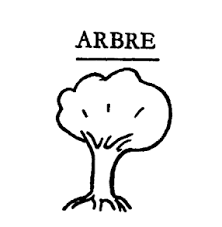
\includegraphics[width=2.06597in,height=2.11319in]{./img1.jpg}

(Lacan, 1956, p. 499, \emph{p. 151}, \emph{p. 502})
\end{center}

\noindent{}(o que, na verdade, está aberto à objeção de parecer reverberar uma
teoria da linguagem baseada na correspondência entre palavras e coisas),
por este modelo (\emph{Ecrits} (1957), p. 499, \emph{p. 151}, \emph{p.
502}):

\begin{center}
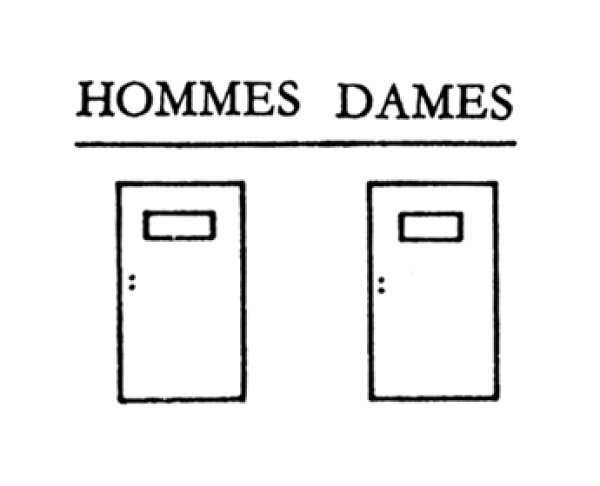
\includegraphics[width=1.72639in,height=1.40556in]{./img2.jpg}
\end{center}

``Qualquer ser falante'' (E, p. 150) deve estar alinhado em um ou outro
lado da divisão.\footnote{Não se trata, portanto, de uma questão de
  filologia e, \emph{então}, do falo, como John Forrester argumenta, mas
  da sexualidade/do falo \emph{como} linguagem (John Forrester,
  ``\emph{Philology and the phallus}'', em MacCabe (1981)).}

A diferença sexual é, então, designada de acordo com o fato de o sujeito
possuir ou não possuir o falo, o que não significa que a diferença
anatômica \emph{é} a diferença sexual (como se uma pudesse ser
estritamente dedutível da outra), mas que essa diferença anatômica vem a
\emph{figurar} a diferença sexual, ou seja, ela se torna o único
representante do que essa diferença pode ser. Ela encobre, assim, a
complexidade da vida sexual inicial da criança com uma oposição crua na
qual essa mesma complexidade é recusada ou reprimida. O falo indica
assim a redução da diferença a uma instância de percepção visível, a um
valor \emph{aparente} {[}\emph{seeming}{]}.

Freud concebeu o momento em que o menino e a menina veem que são
diferentes como um trauma no qual a menina é vista como estando em falta
(muitas vezes as objeções começam aqui). Mas algo só pode \emph{ser
visto} como faltando de acordo com uma hierarquia de valores
pré"-existente (``não falta nada ao real'', \versal{PP}, p. 113). O que conta não
é a percepção, mas o seu sentido já assinalado --- o momento, portanto,
pertence ao simbólico. E, se Lacan sustenta que o uso simbólico do falo
deriva de sua visibilidade (algo pelo quê ele foi frequentemente
criticado), é apenas na medida em que a ordem do visível, a aparência, o
aparente {[}\emph{the seeming}{]}, é objeto de seu ataque. De fato, ele
constantemente recusou uma identificação grosseira do falo com a ordem
do visível ou do real (``pode"-se dizer que esse significante é escolhido
como o que se destaca naquilo que é mais facilmente apreendido no real
da copulação sexual'', \versal{MP}, p. 82), e ele o referiu, em vez disso, a essa
função de ``velamento'' na qual ele localiza a duplicidade fundamental
do signo linguístico:

\begin{quote}
Todas essas proposições apenas ocultam o fato de que o falo só pode
desempenhar seu papel como velado, isto é, como sendo em si mesmo o
signo da latência com a qual tudo que é significável é atingido assim
que é elevado à função de significante. (\versal{MP}, p. 82)
\end{quote}

O sentido só pode ser erigido; ele é estabelecido e fixado. O falo
simboliza os efeitos do significante, pois, na medida em que ele próprio
não tem valor, pode representar aquilo a que o valor se
\emph{acrescenta}.

As afirmações de Lacan sobre a linguagem precisam ser tomadas em duas
direções: a da fixação do próprio sentido (aquilo que se impõe ao
sujeito), e, a despeito dessa mesma fixação, a do ponto de seu
deslizamento constante, o risco ou ponto de fuga que ela sempre contém
(o inconsciente). A sexualidade é situada em ambas essas dimensões ao
mesmo tempo. A dificuldade é manter unidos esses dois direcionamentos ---
a sexualidade no simbólico (uma ordenação), e a sexualidade como aquilo
que falha constantemente. Uma vez que a relação entre esses dois
aspectos da psicanálise pode ser vista, então os termos em que a
sexualidade feminina pode ser descrita sofrem uma mudança radical. O
conceito do simbólico sustenta que a sexualidade da mulher é inseparável
das representações através das quais ela é produzida (``imagens e
símbolos para a mulher não podem ser isolados das imagens e símbolos da
mulher\ldots{} é a representação da sexualidade que condiciona o modo como
ela entra em jogo'', C, p. 90), mas essas mesmas representações irão
revelar a divisão através da qual elas são constituídas enquanto tais. A
questão sobre o que é uma mulher, nesta abordagem, sempre esbarra no
reconhecimento crucial de que não há absolutamente nenhuma garantia de
que ela \emph{é}.\footnote{Cf. seção \versal{II}, abaixo.} Mas, se ela assumir
seu lugar de acordo com o processo descrito, então sua sexualidade
trairá, necessariamente, os impasses de sua história.

A sexualidade pertence, para Lacan, ao reino da mascarada. O termo vem
de Joan Rivière (Rivière, 1929), para quem ele indicava uma feminilidade
fracassada. Para Lacan, a mascarada é a própria definição da
``feminilidade'' precisamente porque ela se constrói em referência a um
signo masculino. A questão da frigidez (da qual, Lacan o reconheceu, a
psicanálise ``desistiu'', C, p. 89) também está presente aqui, e é
descrita em ``A significação do falo'' (\versal{MP}) como o efeito do status do
termo fálico. Mas isso não implica que exista uma fisiologia à qual as
mulheres pudessem, de alguma forma, ser devolvidas, ou com relação à
qual pudessem ser libertadas. Pelo contrário, o termo ``frigidez''
representa, do lado da mulher, a dificuldade inerente à própria
sexualidade, a disjunção sobreposta ao corpo pelo desejo, no ponto em
que ela se inscreve na relação genital. Agora a psicanálise reconhece
que qualquer critério simples da feminilidade em termos de um
deslocamento do prazer do clitóris para a vagina corresponde a uma
farsa, mas o que importa são as fantasias implicadas em cada um deles
(ou em ambos). Para ambos os sexos, a sexualidade tocará necessariamente
a duplicidade que sustenta sua divisão fundamental. No que diz respeito
à feminilidade vaginal ``normal'', que poderia ser tomada como o
reconhecimento do valor do signo masculino (um ``chegar a'' esse
reconhecimento), ela sempre evocará a divisão em que seu valor é erigido
(``por que não reconhecer que, se não há virilidade que a castração não
consagre, então, para a mulher, é um amante castrado ou um homem
morto\ldots{} que se esconde atrás do véu para dali convocar sua adoração''?,
C, p. 95).

A descrição da sexualidade feminina é, portanto, uma exposição dos
termos de sua definição, o exato oposto de uma demanda sobre o que essa
sexualidade deveria ser. Ali onde tal definição é fornecida ---
``identificação com a mãe como desejante e reconhecimento do falo no pai
real'' (Safouan, 1976, p. 110), ela envolve precisamente um colapso do
falo no real e do desejo no reconhecimento ­--- atribuindo um caráter de
mentira, poderíamos dizer, a todo o problema delineado.\footnote{A
  dificuldade desses termos é reconhecida por Safouan, mas o problema
  permanece; cf. também Eugénie Lemoine"-Luccioni, \emph{Partage des
  femmes} (1976), onde há o mesmo colapso entre o Outro a ser
  reconhecido pela mulher em sua entrada no desejo, e o homem real que,
  idealmente, ela vem a aceitar (``O Outro, o homem'', p. 83; ``O Outro,
  o homem como sujeito'', p. 87). Parece haver uma tendência constante a
  tomar literalmente os termos de Lacan e é quando isso acontece que as
  definições mais facilmente reconhecidas como reacionárias tendem a
  aparecer. Podemos ver isso em áreas aparentemente muito diferentes
  como na tradução feita por Maude Mannoni do Nome"-do"-Pai numa prática
  terapêutica que procura estabelecer a genealogia paternal da criança
  psicótica (Mannoni, 1967); e na explicação de Lemoine"-Luccioni do
  Outro real que assegura a castração para a mulher, de outro modo
  condenada ao puro narcisismo. Essa explicação de Lemoine"-Luccioni
  lembra, em muitos aspectos, aquela de Helene Deutsch (1930), que
  descreveu a transição para a feminilidade em termos de um desejo de
  castração que é produzido pelo homem no corpo da mulher.}

\section{II}

Três pontos emergem do que foi descrito até agora:

\begin{enumerate}
\def\labelenumi{\arabic{enumi})}
\item
  a anatomia importa na abordagem: ``para mim `a anatomia não é o
  destino'', mas isso não significa que a anatomia não figura (Safouan,
  1976, p. 131); ela, no entanto, \emph{só figura} (ela é uma
  simulação);\footnote{Como esse trecho guarda muitas ambiguidades,
    difíceis de verter para o português e importantes para o argumento,
    optamos por deixar aqui o registro do original ``anatomy is what
    figures in the account: `for me `anatomy is not destiny', but that
    does not mean that anatomy does not figure (Safouan, 1976, p. 131),
    but it \emph{only figures} (it is a sham)'' (p.~44). {[}\versal{N.~T.}{]}}
\item
  o falo fica por sua própria conta e qualquer privilégio masculino
  erguido sobre ele corresponde a uma impostura; ``o que se pode chamar
  um homem, o ser masculino falante, desaparece estritamente como um
  efeito do discurso,\ldots{} ao ser inscrito nele apenas como castração''
  (\versal{SXVIII}, 12, p. 4);
\item
  a mulher não é inferior, ela é \emph{sujeitada}:
\begin{quote}
Que a mulher seja desta forma introduzida numa ordem de trocas em que
ela é objeto, é isto mesmo que confere o caráter fundamentalmente
conflitual, eu diria sem saída, de sua posição --- a ordem simbólica,
literalmente, a submete, a transcende.

(\ldots{})

Existe para ela, algo de insuperável, de inaceitável, digamos, no fato
de ser posta em posição de objeto numa ordem simbólica, à qual ela está,
por outro lado, inteiramente submetida, assim como o homem (\versal{SII}, pp.
304-5, \emph{p. 329}).
\end{quote}
\end{enumerate}

A força do conceito de simbólico reside em sistematicamente repudiar
qualquer concepção de sexualidade que assuma a natureza pré"-dada da
diferença sexual --- a polêmica concernente à psicanálise e a recusa de
qualquer ``natureza'' por parte do feminismo aparecem da maneira a mais
convergente aqui. Mas um problema permanece. O uso que Lacan fazia do
simbólico nesta fase dependia muito da noção de parentesco de
Lévi"-Strauss, na qual as mulheres são definidas como objetos de troca.
Assim, ele está sujeito às mesmas objeções que a abordagem de
Lévi"-Strauss, na medida em que ela pressupõe a subordinação que pretende
explicar.\footnote{Ver Elizabeth Cowie, ``Woman as Sign'' (1978).}
Assim, embora à primeira vista essas observações de Lacan pareçam mais
críticas da ordem descrita, elas são, em outro sentido, coniventes com
ela e qualquer argumento nelas alicerçado corre o risco de ser
circular.\footnote{Cf., por exemplo, Gayle Rubin, ``The Traffic in Women''
  \emph{in} R. M. Reiter (1975), que descreve a psicanálise como uma
  ``teoria sobre a reprodução do parentesco'', perdendo de vista,
  novamente, o conceito de inconsciente e todo o problema da identidade
  sexual, reduzindo as relações descritas a um conjunto bastante literal
  de atos de troca.}

Penso ser crucial o fato de que Lacan, no momento em que fez essas
observações, dispusesse de um conceito de fala plena, de acesso à ordem
simbólica cujo equivalente subjetivo é um intercâmbio linguístico bem
sucedido (\emph{Ecrits}, (1953)). Mas seu trabalho sofreu uma mudança
que impediu inteiramente qualquer concepção de linguagem como mediação,
em favor de uma crescente ênfase em sua divisão fundamental e nos
efeitos dessa divisão sobre o nível da própria sexualidade.

``Não há relação sexual'': eis a tônica de seu pensamento. ``Não há
relação sexual'' porque o inconsciente divide os sujeitos em si mesmos e
em relação aos outros, e porque é o mito dessa relação que atua como
barreira contra a divisão, estabelecendo uma unidade através da qual
essa divisão é persistentemente denegada {[}\emph{disavowed}{]}. Donde
se segue a fórmula correlata e oposta ``Há do Um'' (as duas fórmulas
devem ser tomadas em conjunto), que se refere a essa fantasiosa unidade
da relação ``\emph{Nós dois somos um só}. Todo mundo sabe, com certeza,
que jamais aconteceu, entre dois, que eles sejam só um, mas, enfim,
\emph{nós dois somos um só}. É daí que parte a ideia do amor {[}\ldots{}{]} o
problema é de como é que pode haver um amor por um outro'' (\versal{SXX}, p. 46,
\emph{pp. 52-3}); passando à supressão da divisão e da diferença (``Ame
o próximo como a si mesmo {[}\ldots{}{]} o mandamento estabelece a abolição
da diferença sexual'' (\versal{SXXI}, 4, p. 3), e à própria ideologia da unidade
e da plenitude, que, para Lacan, apaga a lacuna do desejo humano.

Nos textos iniciais, a unidade era atribuída ao imaginário; o simbólico
era, pelo menos potencialmente, sua ruptura. Nos textos posteriores,
Lacan localizou a fantasia da ``identidade'' {[}\emph{sameness}{]} na
linguagem e na relação sexual, ao mesmo tempo. ``Não há relação sexual''
porque os sujeitos se relacionam através do que faz sentido em
\emph{lalangue}.\footnote{O termo de Lacan para ``\emph{langue}''
  (língua) de Saussure, parte da distinção que este promove entre
  \emph{langue} (a organização formal da linguagem) e \emph{parole}
  (fala), a elocução individual. O termo de Lacan desloca essa oposição
  na medida em que, para ele, a organização da linguagem só pode ser
  compreendida em termos da relação do sujeito com ela. \emph{Lalangue}
  indica a parte da língua que reflete as leis dos processos
  inconscientes, mas cujos efeitos vão além dessa reflexão, e escapam à
  apreensão do sujeito (ver \versal{SXX}, pp. 126-7, pp. 148-9).} Esse ``fazer
sentido'' é um complemento que supre a falta da subjetividade e da
linguagem, do sujeito \emph{na} linguagem, contra a qual ele é colocado.
A psicanálise afirma que o sentido é sexual, mas deixou para trás
qualquer noção de uma sexualidade reprimida que, de alguma forma,
permitiria falar. O sentido só pode ser descrito como sexual levando em
conta os limites do sentido, pois o sentido em si mesmo opera \emph{no}
limite, os limites de seu próprio fracasso: ``O sentido indica a direção
na qual ele falha'' (\versal{\emph{E}}, p. 150). A tônica, portanto, está no
constante fracasso na linguagem e na sexualidade, que significam
tentativas de complementar ou ocultar: ``Tudo o que está implicado na
referência analítica ao comportamento humano supõe, não que o sentido
reflete o sexual, mas que o suplementa'' (\versal{SXXI}, 15, p. 9). A sexualidade
é o ponto de fuga do sentido. O amor, por outro lado, pertence ao
\emph{Lust"-Ich} ou ego"-prazer, que disfarça esse fracasso no reflexo
entre semelhantes (o amor como forma última de auto"-reconhecimento).

Podemos dizer que Lacan tomou a relação entre inconsciente e sexualidade
e a levou ao extremo, oferecendo uma explicação da sexualidade apenas em
termos de divisões --- a divisão \emph{do} sujeito, a divisão
\emph{entre} sujeitos (em oposição à relação). Donde o enfoque crescente
na enunciação,\footnote{O termo vem de Benveniste (Benveniste, 1958), com
  sua distinção entre \emph{énoncé} e \emph{énonciation}, entre o
  sujeito da enunciação o e o sujeito do próprio enunciado. Lacan situa
  o inconsciente na divisão radical destas instâncias, como se vê de
  forma mais transparente na afirmação ``Eu estou mentindo'', onde há
  claramente dois sujeitos, um que está mentindo e outro que não está.}
na divisão interna da linguagem,\footnote{Cf. o grafo em \emph{Feminine
  sexuality in psychoanalytic doctrine}.} e também a formalização
deliberada da explicação --- a diferença sexual como uma divisão, algo a
expor (exatamente uma formalidade, uma questão de forma (o grafo de
\emph{Encore}, \versal{SXX}, \versal{\emph{E}}, p. 149)). O desafio em relação à unidade
do sujeito, à sua aparente coerência, é, então, endereçado ao discurso
da própria sexualidade: ``em lugar de \emph{um} significante que
interrogamos, interrogar o significante \emph{Um}'' (\versal{SXX}, p. 23). Assim,
não há mais ``unidade'' imaginária e, então, diferença ou troca
simbólica, mas antes uma denúncia do simbólico quanto à unidade
imaginária que os seus mitos mais persistentes continuam a promover.

Dentro desse processo, a mulher é construída como uma categoria absoluta
(ao mesmo tempo excluída e elevada), uma categoria que serve para
garantir a unidade do lado do homem. O homem coloca a mulher na base da
sua fantasia, ou constitui sua fantasia através da mulher. Lacan
afastou"-se, portanto, da ideia de um processo problemático, mas
socialmente assegurado, de troca (a mulher como objeto) em nome da
construção da mulher como categoria da linguagem (mulher como \emph{o}
objeto, a fantasia de sua definição). O que é agora exposto nessa
concepção é ``uma transferência, para a mulher, da dificuldade inerente
à própria sexualidade'' (\versal{PP}, p. 118).

Os dois últimos textos traduzidos aqui (\versal{\emph{E}} e \versal{O}) pertencem a esse
desenvolvimento. Eles avançam e podem ser vistos como uma tentativa de
resolver os problemas levantados por aqueles que os precedem. Enquanto
nos textos anteriores a tônica residia na circulação do falo no processo
de troca sexual, nestes afirma"-se efetivamente que, se é o falo que
circula, então não há troca (ou relação). A questão, doravante,
torna"-se, não tanto a ``dificuldade'' da sexualidade feminina que se
segue da divisão fálica, mas o que significa, dada essa divisão, falar
da ``mulher''. Como sugere o autor do primeiro artigo de \emph{Scilicet}
no final do argumento, essa é uma questão, em muitos aspectos, mais
fundamental ou ``radical'':

\begin{quote}
o que quer que possa ser sustentado sobre a constituição da posição
feminina no complexo de Édipo, ou na ``relação'' sexual, apenas diz
respeito a uma segunda etapa, na qual as regras que governam um certo
tipo de troca baseado num valor comum já foram estabelecidas. É num
estágio mais radical, constitutivo daquelas próprias regras elas mesmas,
que Freud aponta para a última questão, indicando que é a mulher que vem
a atuar como seu apoio. (\versal{PP}, p. 118-19)
\end{quote}

Nos textos posteriores, o termo central é o \emph{objeto pequeno a}
{[}\emph{objet a}{]}, a fórmula de Lacan para o objeto perdido que
alicerça a simbolização, a causa e a ``sustentação'' do desejo. Aquilo a
que o homem se relaciona é a esse objeto e o ``todo de sua realização na
relação sexual se resume à fantasia'' (\versal{\emph{E}}, p. 157). Como o lugar
no qual a falta é projetada e, através do qual, é simultaneamente
rejeitada, a mulher é um ``sintoma'' para o homem.

Definida como tal, reduzida a não ser nada mais do que esse lugar
fantasmático, a mulher não existe. A afirmação de Lacan ``Ⱥ mulher não
existe'' é, pois, o corolário de sua acusação contra a fantasia sexual.
Isso significa, não que mulheres não existam, mas que seu status como
categoria absoluta e garantidora da fantasia (exatamente \emph{A}
mulher) é falso (Ⱥ). Lacan vê o amor cortês como elevação da mulher ao
lugar no qual sua ausência ou inacessibilidade sustenta a falta
masculina (``Para o homem, cuja dama era inteiramente, no sentido mais
servil do termo, seu sujeito feminino, o amor cortês é a única maneira
de sair elegantemente da ausência de relação sexual'', \versal{\emph{E}}, p.
141), na medida em que ele vê sua degradação como pré"-condição para a
crença do homem em sua própria alma (``Para que a alma venha a ser, ela,
a mulher, lhe é diferenciada {[}\ldots{}{]} chamada mulher e difamada'',
\versal{\emph{E}}, p.156). Em relação ao homem, a mulher representa tanto a
diferença como a perda: ``De um lado, a mulher torna"-se, ou é produzida,
precisamente, como o que ele não é, isto é, diferença sexual, e, no
outro, como aquilo a que ele tem de renunciar, isto é, gozo'' (\versal{SXVIII},
6, pp. 9-10).\footnote{Ver Otto Fenichel, num artigo ao qual Lacan,
  frequentemente, se referiu, sobre a recusa da diferença que sustenta a
  equação menina = falo, frequentemente localizada como uma fantasia
  masculina: ``a diferença das mulheres é negada em ambos os casos; num
      caso, na tentativa de reprimir inteiramente as mulheres, no outro, na
      negação da sua individualidade'' (Fenichel, 1949, p.~13).}

Nos termos da definição fálica, a mulher é constituída como ``não
toda'', na medida em que a função fálica depende de uma exceção (o
``não'') que lhe é atribuída. A mulher é excluída \emph{pela} natureza
das palavras, o que significa que a definição a coloca como exclusão.
Note"-se que não é a mesma coisa dizer que a mulher é excluída \emph{da}
natureza das palavras, uma leitura equivocada que leva à reformulação de
todo o problema em termos do lugar da mulher fora da linguagem, e a
ideia de que as mulheres podem ter, de si próprias, uma fala
completamente diferente.

Para Lacan, homens e mulheres estão, sempre, na linguagem (``(\ldots{}) o que
se suporta sob a função do significante, de \emph{homem}, e de
\emph{mulher}, são apenas significantes absolutamente ligados ao uso
\emph{discorrente} da linguagem'', \versal{SXX}, p. 36, \emph{p. 40}). Todos os
falantes devem alinhar"-se a um lado ou outro desta divisão, mas qualquer
um pode atravessá"-la e inscrever"-se no lado oposto daquele a que está
anatomicamente destinado.\footnote{Note"-se como isso simultaneamente
  altera o conceito de bissexualidade --- não mais uma natureza sexual
  indiferenciada anterior à diferença simbólica (sentido inicialmente
  assumido por Freud), mas como disponibilidade de ambas as posições
  para todos os sujeitos em relação à própria diferença.} Poderíamos
dizer que se trata de uma situação e/ou, mas uma cuja natureza
fantasmática foi infinitamente reiterada por Lacan: ``Não podemos nos
satisfazer com estes encaminhamentos, ao ponto de podermos dizer que o
inconsciente se define tão somente pelo fato de que ele tem uma ideia
muito mais clara a respeito do que se passa aí do que a verdade de que o
homem não é a mulher'' (\versal{SXXI}, 6, p. 9).

A mulher, portanto, \emph{não} é, pois ela é definida puramente por
oposição ao homem (ela é o negativo dessa definição: ``o homem é não
mulher''), e também pelo fato de essa mesma definição ser designada como
fantasia, um conjunto que pode muito bem ser vazio (a referência à
teoria dos conjuntos no seminário de \emph{Ornicar}? Traduzido aqui
(\emph{O})). Se a mulher é ``não toda'', escreve Lacan, então ``ela''
dificilmente poderia se referir a todas as mulheres.

Como negativo do homem, a mulher torna"-se um objeto total de fantasia
(ou um objeto da fantasia totalizante), elevada ao lugar do Outro e
conduzida a se colocar no lugar de sua verdade. Uma vez que o lugar do
Outro é também o lugar de Deus, esta é a forma última da mistificação
(``quanto mais o homem confundir a mulher com Deus\ldots{} menos ele é'',
\versal{\emph{E}}, p. 160). Na medida em que Deus ``não fez a sua saída''
(\versal{\emph{E}}, p. 154), a mulher torna"-se o suporte de seu lugar simbólico.
Em sua obra tardia, Lacan definiu o objetivo da psicanálise como o de
dissolver a confusão por trás dessa mistificação, uma ruptura entre o
\emph{objeto a} e o Outro, cuja fusão ele viu como a elevação da
fantasia à ordem da verdade. O \emph{objeto a}, causa do desejo e
suporte da fantasia masculina, é transposto para a imagem da mulher como
Outro que, então, age como sua garantia. A ``Outridade''
{[}\emph{Otherness}{]} absoluta da mulher, portanto, serve para
assegurar ao homem seu próprio autoconhecimento e verdade. Cabe lembrar
que, para Lacan, não pode haver tal garantia --- não há `Outro do Outro'.
Sua rejeição da categoria ``Mulher'', portanto, pertencia ao âmbito de
seu ataque a qualquer crença injustificável no Outro como tal: ``Este Ⱥ
{[}da mulher{]} barrado\ldots{} relaciona"-se com o significante O quando ele
é barrado (Ø)'' (\versal{\emph{E}}, p. 151).

Isso levou Lacan a desafiar cada vez mais as noções de ``saber'' e
``crença'' e os mitos nos quais elas necessariamente se esteiam. Todas
as afirmações de Lacan que, nos dois últimos dois textos traduzidos aqui
se colocam contra a crença na mulher, contra o seu status de saber, por
problemáticas que sejam, só podem ser entendidas como parte desta
recorrente barra sobreposta aos termos nos quais elas se baseiam. Nesses
últimos textos, Lacan retorna continuamente ao ``sujeito suposto
saber'', à reivindicação de um sujeito que sabe (à reivindicação de
conhecer a si próprio como sujeito) e às diferentes formas de discurso
que podem ser organizadas em torno dessa posição.\footnote{Grande parte
  das dificuldades da obra de Lacan resultou de sua tentativa de
  subverter essa posição a partir de dentro da sua própria expressão
  para reencontrar o lugar de ``não"-saber'' com que ele designou o
  inconsciente; por conta do caráter constantemente escorregadio ou
  fugidio de sua fala, ele acabou por minar a verdadeira mestria que a
  sua própria posição como falante (mestre e analista) necessariamente
  constrói. De fato, pode"-se conduzir, com o enunciado ``Eu não sei'', a
  mesma operação que Lacan realiza com a declaração ``Eu estou
  mentindo'' (cf. nota 21, acima); pois, se eu não sei, então como sei o
  suficiente para saber que não sei e, se sei que não sei, então não é
  verdade que não sei. Lacan, sem dúvida, ficou preso nesse paradoxo de
  sua própria declaração.} ``Saber'' é apenas uma pretensão, assim como
a ``crença'' repousa inteiramente na suposição do que é falso. Acreditar
n'A Mulher é simplesmente uma forma de cobrir a divisão ou incerteza que
também sustenta a convicção como tal. E, quando Lacan diz que as
mulheres não sabem, na medida em que, num certo registro, ele relegue as
mulheres para um domínio externo e contrário ao de sua própria {[}de
Lacan{]} afirmação, ele também reconhece a vinculação disso com os
parâmetros do próprio saber ou com a restrição deles (``o saber é
irremediavelmente uma errância'', \versal{SXXI}, 6, p. 11).

O Outro barrado (Ø) coloca"-se contra esse conhecimento e como lugar da
divisão onde o sentido vacila, onde ele escorrega e se desloca. Este é o
lugar da significância {[}\emph{signifiance}{]}, termo de Lacan para
esse mesmo movimento, na linguagem, de distanciamento das posições de
coerência que a linguagem, simultaneamente, constrói. O Outro, portanto,
coloca"-se contra o falo --- sua pretensão de produzir sentido e sua falsa
consistência. É no Outro que o falo busca autoridade e isso lhe é
recusado.

A mulher pertence ao lado do Outro neste segundo sentido, pois, na
medida em que o gozo é definido como fálico, pode"-se dizer que ela
pertence a outro lugar. A mulher está implicada, necessariamente, na
sexualidade fálica, mas ao mesmo tempo é ``em outro lugar que ela
sustenta a questão de seu próprio gozo'' (\versal{PP}, p. 121), ou seja, a
questão sobre seu status como sujeito desejante. Lacan designa este gozo
como suplementar para evitar qualquer noção de complemento, da mulher
como um complemento à natureza fálica do homem (que é precisamente a
fantasia). Mas isso corresponde também ao reconhecimento de algo ``a
mais'', do ``mais de gozar'',\footnote{Por vezes o gozo opõe"-se à ideia
  de prazer como lugar desse excesso; mas onde o gozo é definido como
  fálico, Lacan introduz o conceito de suplemento (``mais de'') que se
  opõe a ele.} que Lacan situa no conceito freudiano de repetição --- o
que escapa ou sobra da função fálica e excede seus limites. A mulher é,
portanto, colocada \emph{além} (além do falo). Esse ``além'' refere"-se
imediatamente à sua mais completa mistificação como Outro absoluto (e,
portanto, nada mais que outro), e a uma \emph{questão}, a questão do seu
próprio gozo, do seu maior ou menor acesso ao resíduo da dialética a que
está constantemente sujeita. O problema é que, uma vez que a noção de
``mulher'' tenha sido tão implacavelmente exposta como uma fantasia,
então é quase impossível colocar uma pergunta desse tipo.

A referência de Lacan à mulher como Outro precisa, pois, ser vista como
uma tentativa de separar dois momentos que estão em constante perigo de
colapsar um no outro --- aquele que atribui à mulher o lugar negativo de
seu próprio sistema (fálico), e aquele que pergunta se as mulheres
podem, como um efeito próprio dessa partilha, romper com e ir além desse
próprio sistema. Para Lacan, essa ruptura é sempre uma ruptura na
linguagem, é a ruptura do sujeito \emph{na} linguagem. O conceito de
gozo (o que escapa na sexualidade) e o conceito de \emph{significância}
(o que se desloca na linguagem) são inseparáveis.

Apenas quando percebemos isso é que podemos localizar adequadamente a
tensão que percorre os capítulos, aqui traduzidos, do Seminário \versal{XX} de
Lacan, \emph{Encore} (\versal{\emph{E}}), tensão entre sua crítica às formas de
mistificação latentes à categoria Mulher e a reiterada pergunta sobre o
que poderia ser sua ``outridade''. Uma tensão que pode ser reconhecida
na própria pergunta ``O que quer uma mulher?'', na qual Freud se deteve
e para a qual Lacan retornou. Essa tensão é mais evidente no recurso de
Lacan a Santa Teresa, cuja estátua de Bernini em Roma\footnote{``Qual é
  o seu \emph{gozo}, de onde \emph{vem}? (\versal{\emph{E}}, p. 147) --- uma
  pergunta, aparentemente redundante, feita pelo anjo cuja flecha está
  posicionada acima dela (a ``perfuração'' {[}\emph{piercing}{]} de
  Santa Teresa), e cuja natureza problemática é melhor ilustrada pelos
  cardeais e doges perfilados na galeria do ``proscênio'' ---
  \emph{testemunhas} da encenação de um ato que, por causa das linhas
  perspectivas, eles não podem, de fato, \emph{ver} (Bernini, \emph{O
  êxtase de Santa Teresa}, Santa Maria della Vittoria, Roma).} ele tomou
como modelo para um outro gozo --- a mulher, portanto, como ``mística'',
mas, ele insistiu, isto não é ``não político'' (\versal{\emph{E}}, p. 146), na
medida em que o misticismo é uma das formas de expressão disponíveis
quando essa ``outridade'' na sexualidade expressa sua denúncia mais
contundente. E, se avançarmos do momento do recurso de Lacan à sua
imagem como executada pelo homem aos próprios escritos de Santa Teresa,
ao seu comentário sobre ``O cântico dos cânticos'', encontramos essa
sexualidade na forma de uma perturbação que, crucialmente, ela situa não
no nível do conteúdo sexual do cântico, mas naquele de sua enunciação,
na instabilidade de seus pronomes --- uma precariedade na linguagem que
revela que nem o sujeito nem Deus podem ocupar seu lugar (``falando com
uma pessoa, pedindo a outra pela paz e, então, falando com a pessoa em
cuja presença ela está'' (Santa Teresa, 1946, p. 359)).\footnote{Comentário
  sobre a linha do ``Cântico dos cânticos'': ``Que o Senhor me beije com
  o beijo da sua boca, porque teus seios são mais doces do que o
  vinho''. {[}\emph{``Let the Lord kiss me with the kiss of his mouth,
  for thy breasts are sweeter than wine''}.{]}} A sexualidade pertence,
portanto, ao nível de seu deslizamento {[}\emph{shifting}{]} e do
deslizamento do sujeito.

No final de sua obra, Lacan falou da natureza ``anti"-fálica'' da mulher,
deixando"-a aberta àquilo ``que do inconsciente não pode ser dito''
(\emph{Ornicar?}, 20-1, p. 12) (referência às mulheres analistas nas
quais podemos reconhecer, ironicamente, o eco da convicção de Freud de
que elas teriam acesso a um estrato diferente da vida
psíquica).\footnote{No momento em que escrevia isso, Lacan tinha acabado
  de dissolver sua escola em Paris, fazendo convergir à declaração com a
  qual representou esse ato --- ``\emph{Je père"-sévère}'' (``\emph{Eu
  persevero}''; o trocadilho está em ``\emph{per}'' e ``\emph{père}''
  (pai)) --- todo o problema da autoridade e da paternidade que
  atravessou a história institucional de seu trabalho. Do precoce
  posicionamento contra um contexto que ele (e outros) considerava
  autoritário, e do cancelamento, como seu efeito, de seu seminário
  \emph{O nome do pai,} de 1953, à questão da autoridade e da
  transferência, que estava por trás da ruptura seguinte, em 1964, e que
  emerge muito claramente nessa dissolução. Tem sido um paradoxo
  inesgotável da posição de Lacan o fato de que ele forneceu a crítica
  mais sistemática das formas de identificação e de transferência ao
  mesmo tempo em que, em virtude deste mesmo fato, ele representou
  largamente tais formas. Que um número de mulheres analistas (cf. nota
  30, abaixo) descobriu que sua posição, em relação a isso, seria
  impossível, apenas confirma a estreita relação entre a questão da
  sexualidade feminina e as divisões e dificuldades institucionais da
  própria psicanálise.} Em relação aos textos anteriores, poderíamos
dizer que a mulher já não constrói mascaradas, ela \emph{falta}: ``o
gozo da mulher não vem sem dizer, isto é, sem dizer da verdade'', ao
passo que, para o homem, ``seu gozo basta e é precisamente por isso que
ele não entende nada'' (\versal{SXXI}, 7, p. 16). Aqui há um risco de devolver à
mulher um estatuto de verdade (a mitologia tão denunciada). Mas, para
Lacan, essa ``verdade'' do inconsciente é apenas aquele momento da
divisão fundamental pela qual o sujeito entrou na linguagem e na
sexualidade e o constante fracasso da localização em ambas.

Esta é a força da argumentação de Lacan: sua insistência no fato de que
a feminilidade só pode ser compreendida nos termos de sua construção,
uma insistência que produziu como resposta o mesmo restabelecimento das
mulheres, o mesmo argumento em favor de \emph{sua} natureza sexual, que
aquele visto nas décadas de 1920 e 1930 em resposta a Freud. Dessa vez,
a questão da simbolização, que, como defendemos, estava latente no
debate anterior, esteve no centro da resposta. Isso é tanto mais
evidente na medida em que a especificidade da sexualidade feminina na
discussão mais recente\footnote{Nesta última seção, vou me referir
  predominantemente aos trabalhos de Michèle Montrelay e Luce Irigaray.
  A primeira foi membro da escola de Lacan, antes da sua dissolução em
  Janeiro de 1980, quando se afastou dele; a segunda trabalhou em sua
  escola até 1974, quando, com a publicação de seu livro \emph{Speculum
  de l´autre femme} (1974), foi demitida do departamento de psicanálise
  da Universidade de Paris \versal{VIII} (Vincennes), há pouco reorganizado.
  Ambas são psicanalistas praticantes. Montrelay retoma a controvérsia
  Freud"-Jones especificamente quanto ao acesso das mulheres à linguagem
  em seu artigo ``Investigação sobre a feminilidade'' (1970 (1978)). O
  livro de Irigaray, \emph{Speculum}, continha uma crítica aos trabalhos
  de Freud sobre a feminilidade; seu mais recente \emph{Ce sexe qui n'en
  est pas un} (1977) contém um capítulo (``\emph{Cosi fan tutti}'')
  diretamente endereçado ao \emph{Encore} de Lacan, \versal{SXX}.} tornou"-se,
explicitamente, a questão da relação das mulheres com a linguagem. Uma
vez que é a ordem da linguagem que estrutura a sexualidade em torno do
termo masculino --- ou o privilégio desse termo que mostra a sexualidade
como construída dentro da linguagem ---, emerge a questão da relação da
mulher com essa linguagem e, simultaneamente, com essa sexualidade. A
questão do corpo da menina (o que ela pode ou não saber sobre ele), tal
como referido no debate anterior, passa a ser a questão do corpo da
mulher como linguagem (o que, desse corpo, pode alcançar simbolização).
O objetivo é resgatar a mulher do domínio do termo fálico e da
linguagem, ao mesmo tempo. O que significa que a feminilidade é
vinculada a um ponto de origem que é anterior à marca da diferença
simbólica e da lei. A relação privilegiada das mulheres com esse momento
original fornece"-lhes acesso a uma forma arcaica de expressividade, fora
do circuito da troca linguística.

Esse momento de origem é o corpo materno, um espaço indiferenciado e,
ainda assim, um espaço em que a menina se reconhece a si mesma. A
menina, então, tem de suprimir ou desvalorizar essa plenitude de
reconhecimento para se alinhar à ordem do termo fálico. No argumento em
favor de uma feminilidade primordial, fica claro que a relação entre mãe
e criança é concebida como diádica e simplesmente reflexiva (um para um
--- a menina se \emph{conhece} plenamente na mãe), o que, mais uma vez,
impossibilita o conceito de desejo. A especificidade feminina implica
diretamente, portanto, o conceito de uma relação imediata e não
problemática com a origem.

As posições assumidas não são idênticas, mas compartilham a ênfase na
especificidade das pulsões femininas, uma ênfase que estava na base da
resposta anterior a Freud. Elas extraem parte de seus conceitos
diretamente desse debate (o conceito de pulsões femininas concêntricas
em Montrelay advém, diretamente, de Jones e Klein). Mas os efeitos do
posicionamento são diferentes. Assim, enquanto para Jones, por exemplo,
essas pulsões, idealmente, anteciparam e asseguraram a identidade
heterossexual da criança do sexo feminino, agora essas mesmas pulsões
colocam em risco seu acesso a qualquer objeto (Montrelay),\footnote{Montrelay
  tenta resolver a controvérsia ``Freud"-Jones'' tornando as duas
  explicações distintas da feminilidade equivalentes a \emph{estágios}
  do desenvolvimento psicossexual da menina, sendo a feminilidade
  definida como a passagem de uma economia concêntrica para outra na
  qual a castração simbólica entra em jogo. O acesso à simbolização
  depende da transição, e é onde ele falha que a mulher permanece
  vinculada a uma catexia primordial da linguagem como extensão do corpo
  materno indiferenciado. Montrelay deve, portanto, ser crucialmente
  distinguida de Irigaray neste ponto, uma vez que, para ela, tal
  fracasso precipita a ansiedade e não é, em nenhum sentido, um conceito
  de feminilidade que ela pretende promover.} ou então asseguram a
mulher para si mesma e, através disso, para outras mulheres (Irigaray).
As mulheres são \emph{remetidas}, portanto, na explicação, umas às
outras --- contra o termo fálico, mas também contra a perda da origem,
que a explicação de Lacan parece implicar. É, portanto, uma recusa da
divisão que dá, à mulher, acesso a um estrato diferente da linguagem,
onde as palavras e as coisas não são diferenciadas, e o real do corpo
materno ameaça ou impede o acesso da mulher à proibição e à lei.

Há uma força nessa explicação que foi reconhecida pelo feminismo. Na sua
forma mais vigorosa, expressa um protesto engendrado pelo próprio peso
do que Freud e, depois, Lacan descrevem (é o \emph{efeito} dessa
descrição).\footnote{Note"-se também o fácil deslizamento do título de
  Irigaray, \emph{Ce sexe qui n'en est pas un}, ``Este sexo que não é
  um'', frente à fórmula de Lacan, ``Este sexo que não é \emph{um}''.}
E algo de sua posição estava certamente presente nos textos anteriores
de Lacan (``a sexualidade feminina\ldots{} como o esforço de um gozo envolto
em sua própria contiguidade'', C, p. 97). Mas Lacan voltou a essa
resposta no textos posteriores, que podem, portanto, ser vistos como uma
espécie de réplica, assim como os trabalhos de Freud de 1931 e 1933
sobre a feminilidade se endereçaram a algumas das críticas que ele havia
recebido.

Para Lacan, como vimos, não há realidade pré"-discursiva (``Como
retornar, senão por um discurso especial, a uma realidade
pré"-discursiva?'', \versal{SXX}, p. 33, \emph{p. 37}), nenhum lugar prévio à lei
que estivesse disponível e pudesse ser recuperado. E não há feminino
fora da linguagem. Primeiro, porque o inconsciente afasta o sujeito de
qualquer relação imediata com o corpo como tal (``não há nada no
inconsciente que esteja de acordo com o corpo'', O, p. 165), e, em
segundo lugar, porque o ``feminino'' é constituído como uma divisão na
linguagem, uma divisão que produz o feminino como seu termo negativo. Se
a mulher é definida como outro é porque a definição a produz como outro,
e não porque ela tivesse outra essência. Lacan não recusa a diferença
(``se não houvesse diferença, como eu poderia dizer que não há relação
sexual'', \versal{SXXI}, 4, p. 18), mas, para ele, o que deve ser questionado é a
aparente ``consistência'' dessa diferença --- do corpo ou de qualquer
outra coisa ---, a divisão que impõe, as definições de mulher que produz.

Para Lacan, dizer que a diferença é diferença ``fálica'' é expor a
natureza simbólica e arbitrária dessa divisão como tal. E é crucial ---
algo que pode ser visto, ainda mais claramente, na resposta aos textos
aqui traduzidos\footnote{Referência ao volume \emph{Feminine sexuality}.}
--- que a recusa do termo fálico traga consigo uma tentativa de
reconstituir uma forma de subjetividade livre da divisão e, portanto,
uma recusa da própria noção de simbolização. Se se trata de desafiar o
estatuto do falo, isso não pode, portanto, originar"-se diretamente do
corpo feminino, mas deve se dar através de um termo simbólico diferente
(caso em que a relação com o corpo é, imediatamente, lançada em crise),
ou, então, através de uma lógica completamente diferente (caso em que já
não se está de modo algum na ordem da simbolização).

As reivindicações feitas contra Lacan colapsam, portanto, em dois níveis
diferentes de objeção: que o corpo deve ser mediado pela linguagem e que
o termo privilegiado dessa mediação é masculino. O fato de que a recusa
do falo se revele, mais uma vez, como uma recusa do simbólico não
encerra, mas deixa em aberto, e ainda sem resposta, a questão de saber
por que razão essa simbolização necessária e o estatuto privilegiado do
falo aparecem como interdependentes na estruturação e garantia (nunca
assegurada) da subjetividade humana.

Não se trata aqui, portanto, de negar que Lacan estava implicado com o
falocentrismo que ele descreveu, nem que suas próprias expressões
reenviam constantemente à mestria {[}\emph{mastery}{]} que ele procurava
minar. A questão do inconsciente e da sexualidade, o movimento em
direção a eles e contra eles, operou exatamente neste nível de sua
própria fala. Mas, para Lacan, ambos funcionam como a questão dessa
fala, e não podem ser remetidos a um corpo fora da linguagem, a um lugar
para o qual o ``feminino'', e, através dele, as mulheres poderiam
escapar. Na resposta a Lacan, portanto, o ``feminino'' retorna, como nos
anos 1920 e 1930, na réplica a Freud, mas, desta vez, acrescido do
sentido de uma resistência a uma organização fálica da sexualidade, que
é reconhecida como tal. O ``feminino'' representa uma recusa dessa
organização, de sua ordenação, de sua identidade. Para Lacan, por outro
lado, interrogar essa mesma organização desautoriza qualquer definição
absoluta do ``feminino''.

A psicanálise não produz essa definição. Ela dá conta de como essa
definição é produzida. Embora a objeção a seu termo dominante deva ser
reconhecida, ela não pode ser respondida com uma explicação que retorne
a um conceito do feminino como pré"-existente, nem com um recurso
imperativo a um androcentrismo no simbólico, que o falo simplesmente
refletiria. A primeira resposta conduziria as mulheres para fora da
linguagem e da história, a segunda simplesmente as subordinaria a ambas.

Nesses textos, Lacan dá"-se conta de como o estatuto do falo na
sexualidade humana impõe à mulher uma definição na qual ela é,
simultaneamente, sintoma e mito. Enquanto continuarmos a sentir os
efeitos dessa definição não podemos nos dar ao luxo de ignorar essa
descrição da impostura fundamental que a sustenta.

\section{Referências bibliográficas}

\versal{BENVENISTE}, É. ``La nature des pronoms''. Em: \emph{Problèmes de
linguistique générale}. Paris: Gallimard, 1966, pp. 251-7.
\emph{Problems in general linguistics}. Florida: University of Miami
Press, 1971, pp 217-22.

\versal{BENVENISTE}, É. ``De la subjectivité dans le langage'' (1958).
\emph{Problèmes}, pp. 258-66. \emph{Problems}, pp. 223-30.

\versal{CHODOROW}, N. \emph{The reproduction of mothering -- Psychoanalysis and
the sociology of gender}. Londres: University of California Press,
1979.

\versal{COWIE}, E. ``Woman as sign'', \emph{m/f}, \versal{I}, 1978, pp. 49-63.

\versal{DEUTSCH}, H. ``The significance of masochism in the mental life of women'',
\emph{\versal{IJPA}}, \versal{XI}, 1930, pp. 48-60.

\versal{FENICHEL}, O. ``The symbolic equation girl = phallus'', \emph{\versal{PQ}}, \versal{XVIII}
(3), 1949, pp. 303-21.

\versal{FREUD}, S. \& \versal{BREUER}, J. \emph{Studies on hysteria} (\versal{SE}, \versal{II}, 1893-5).

\versal{FREUD}, S. (1895) ``Project for a scientific psychology''. (\versal{SE, I}).

\versal{FREUD}, S. \emph{Three essays on the theory of sexuality} (\versal{SE, VII},
1905), pp. 123-245.

\versal{FREUD}, S. (1912) ``On the universal tendency to debasement in the sphere
of love'' (Contributions to the psychology of love, \versal{II}) (\versal{SE}, \versal{XI}, 1912),
pp. 177-90. ``Contribuições para a psicologia da vida amorosa -- Sobre a
mais geral degradação na vida amorosa''. Em: \emph{Amor, sexualidade
feminilidade}. (Trad.: M. R. S. Moraes'. Belo Horizonte: Autêntica,
2018, pp. 137-154.

\versal{FREUD}, S. (1920) \emph{Beyond the pleasure principle}. (\versal{SE}, \versal{XVIII}), pp.
3-64.

\versal{FREUD}, S. ({[}1938{]}1940) ``Splitting of the Ego in the process of
defence'' (\versal{SE}, \versal{XXIII}), pp. 273-8.

\versal{IRIGARAY}, L. \emph{Speculum de l'autre femme}. Paris: Minuit, 1974.

\versal{IRIGARAY}, L. \emph{Ce sex qui n'en est pas un}. Paris: Minuit, 1977.

\versal{JONES}, E. ``The early development of female sexuality''. Em:
\emph{\versal{IJPA}}, \versal{VIII}, 1927, pp. 459-72.

\versal{JONES}, E. ``The theory of symbolism''. Em: \emph{British journal of
psychoanalysis}, \versal{IX} (2), 1916, pp. 181-229.

\versal{KLEIN}, M. ``The importance of symbol formation in the development of the
ego''. Em: \emph{\versal{IJPA}}, \versal{IX}, 1930, pp. 23-39. 1930

\versal{LACAN}, J. (1936) ``Le stade du mirroir comme formateur de la fonction du
Je''. Em: \emph{Écrits}. Paris: Seuil, 1966. \emph{Ecrits: A
selection} (Trad. A. Sheridan). Londres: Tavistock, 1977, pp. 1-7.
\emph{Escritos}. (Trad. Vera Ribeiro) Rio de Janeiro: Zahar, 1998,
pp. 96-103.

\versal{LACAN}, J. ``Cure psychanalytique à l'aide de la poupée fleur.'' Em:
\emph{Comptes rendus, réunion 18 October, Revue française de la
psychanalyse}, 4, Out"-Dez, 1949, p. 567.

\versal{LACAN}, J. ``Fonction et champ de la parole et du langage en
psychanalyse'', (1953) \emph{Ecrits}, pp. 237-322; \emph{Ecrits: A
selection}, pp. 30-113.

\versal{LACAN}, J. \emph{Le moi dans la théorie de Freud et dans la technique de
la psychanalyse}. Le séminaire \versal{II}, 1954-55. Paris: Seuil, 1978. \emph{O
eu na teoria de Freud e na técnica da psicanálise}. (Trad.: M. C. L.
Penot e A. L. Q. de Andrade). Rio de Janeiro: Zahar, 1985.

\versal{LACAN}, J. ``D'une question préliminaire à tout traitement possible de la
psychose'', (1955-6). \emph{Ecrits}, pp. 531-83; \emph{Ecrits: A
selection}, pp. 179-225. \emph{Escritos} (Trad. V. Ribeiro). Rio de
Janeiro: Zahar, 1998, pp. 537-90)

\versal{LACAN}, J. ``Les formations de l'inconscient'' (1957-8). \emph{Bulletin de
psychologie}, \versal{II}, pp. 1-15.

\versal{LACAN}, L. (1959) ``À la mémoire d'Ernst Jones: Sur sa théorie de
symbolisme''. Em: Ecrits, pp. 697-717. ``À memória de Ernst Jones: Sobre
sua teoria do simbolismo.'' \emph{Escritos}. (Trad. Vera Ribeiro) Rio
de Janeiro: Kahar, 1998, pp. 704-25)

\versal{LACAN}, J. (1960) ``Guiding remarks for a congress on feminine sexuality''
(Trad. J. Rose) Em: \emph{Feminine sexuality -- Jacques Lacan and the
école freudienne} (Ed. J. Mitchell e J. Rose; Trad. J. Rose).
Londres: The Macmillan press \versal{LTD}, 1982.

\versal{LACAN}, J. \emph{Les quatres concepts fondamentaux de la psychanalyse}:
Le séminaire \versal{XI}, (1964) (a), (Paris: Seuil, 1973). \emph{The four
fundamental concepts of Psycho"-Analysis}, (Trad. A. Sheridan, ed.:
J.-A. Miller). London: Hogarth, 1977. \emph{Os quatro conceitos
fundamentais da psicanálise} (Trad. M. D. Magno). Rio de Janeiro:
Zahar, 1988.

\versal{LACAN}, J. \emph{Encore}: Le séminaire \versal{XX}, 1972-3. Paris: Seuil, 1975.
\emph{Mais, ainda} (Trad. M. D. Magno) Rio de Janeiro: Zahar, 2008.

\versal{LACAN}, J. ``Les non"-dupes errent'': Le séminaire \versal{XXI}, 1973-4 (manuscrito
inédito).

\versal{LACAN}, J. \emph{Scilicet}, review of \emph{le champ freudien}, \versal{I"-VII}.
Paris: Seuil, 1968-76.

\versal{LACAN}, J. \emph{Ornicar?} \emph{Periodical of} le champ freudien. Dept
of Psycho"-Analysis at Paris \versal{VII} (Vincennes). Paris: le graphe, no. 1 --
1975- ).

\versal{LEMOINE"-LUCCIONI}, E. \emph{Partage des femmes, (le champ freudien)}.
Paris: Seuil, 1976.

\versal{MacCABE}, C. (ed.) \emph{The talking cure -- Essays in psychoanalysis and
language}. Londres: Macmillan, 1981.

\versal{MANNONI}, M. \emph{L'enfant, sa ``maladie'' et les autres, (le champ
freudien)}. Paris: Seuil, 1967. \emph{The child, his illness and the
others}. Londres: Tavistock, 1970.

\versal{MONTRELAY}, M. ``Recherches sur la femininité''. \emph{Critique}, \versal{XXVI},
Paris, 1970, pp. 654-74. Edição revista: ``Inquiry into femininity'',
(Trad. E Introdução: Parveen Adams, \emph{m/f}, \versal{I}, 1978, pp. 65-101.

\versal{RIVIÈRE}, J. ``Womanliness as mascarade'', \emph{\versal{IJPA}}, \versal{X}, 1929, pp.
303-13.

\versal{RUBIN}, G. ``The Traffic in Women: Notes on the 'Political Economy' of
Sex''. Em: Rayna R. Reiter (ed.), \emph{Toward an Anthropology of
Women}. Monthly Review Press, 1975, pp. 157-210.

\versal{SAFOUAN}, M. \emph{Etudes sur l'Óedipe}, (\emph{le champ freudien}).
Paris: Seuil, 1974. ``Is the Oedipus complex universal?'' (Trad. B.
Brewster), \emph{m/f}, 5-6, 1981, pp. 83-90.

\versal{SAUSSURE}, F. de. \emph{Cours de linguistique générale (1915)} (Ed.:
Tullio de Mauro). Paris: Payot, 1972. \emph{Course in general
linguistics} (revised ed.). Londres; Fontana, 1974.

\versal{SEGALL}, H. ``Notes os symbol formation'', \emph{\versal{IJPA}}, \versal{XXXVIII}, 1957,
pp. 391-7.

\versal{STOLLER}, R. ``A contribution to the study of gender identity'',
\emph{\versal{IJPA}}, \versal{XLV}, 1965, pp. 220-6.

\versal{WINNICOTT}, D. ``1967) ``Mirror"-role of the mother and family in child
development''. Em: \emph{Playing and reality}. Londres: Tavistock, 1971,
pp. 111-18.

\chapter*{Imposições sexuais e diferenças entre os sexos -- Bruxas,
\emph{femmes seules}, solteironas e Sigmund Freud}
\addcontentsline{toc}{chapter}{Imposições sexuais e diferenças entre os sexos -- Bruxas,
\emph{femmes seules}, solteironas e Sigmund Freud, \footnotesize\emph{por Beatriz Santos}}
\hedramarkboth{Imposições sexuais e diferenças entre os sexos}{}


\begin{flushright}
\emph{Beatriz Santos}\footnote{Psicanalista, Professora do Departamento de Estudos Psicanalíticos da Université Paris Diderot (Université de Paris).}
\end{flushright}


Em 1980, a poeta, ensaísta e feminista Adrienne Rich publicou um artigo
questionando o que chamou de ``heterocentrismo não"-examinado'' da
literatura feminista produzida até então. Trata"-se de um texto que se
tornou um clássico da segunda onda do feminismo, \emph{Compulsory
Heterosexuality and Lesbian Existence}\footnote{A. Rich, ``Compulsory
  Heterosexuality and Lesbian Existence (1980)'' In Journal of Women's
  History, Vol. 15, N. 3, pp. 11-48, autumn 2003.
  Traduzido em português como ``Heterossexualidade compulsória e
  existência lésbica'' em Bagoas -- Estudos gays: gêneros e sexualidades,
  v. 4, n. 05, 27 nov. 2012.} e que até hoje é bastante lido e discutido
em disciplinas de Estudos de Gênero. Partindo de uma preocupação quanto
ao modo como a existência lésbica é retratada (ou, justamente, ignorada)
mesmo em obras feministas, Adrienne Rich se dispõe a produzir uma
crítica do que chama de ``orientação heterossexual compulsória'' para
mulheres. Em outras palavras, intenta pensar a distinção entre
homossexualidade e heterossexualidade não em termos de ``preferência''
ou ``escolha'', mas sim em termos de uma orientação \emph{política}.
Para a autora, ainda que muitos trabalhos teóricos sobre a condição das
mulheres apresentem a ideia de que as relações sociais entre os sexos
sejam confusas, extremamente problemáticas e muitas vezes incapacitantes
para as mulheres, quase nunca questionam se em um contexto diferente
mulheres \emph{escolheriam} as uniões heterossexuais e o
casamento.\footnote{Rich (2012), p. 22.}

Há, segundo o trabalho da autora, uma ``naturalização'' da
heterossexualidade como ``preferência sexual'' da maioria das mulheres:
mesmo em estudos que questionam aspectos importantes de suas vidas, tais
como a maternidade, os papéis atribuídos a cada gênero,as regras que
permeiam a construção de relacionamentos, não é questionada uma certa
ideia de preferência ou de orientação sexual nata. Até o início da
década de oitenta, quando começou a escrever sobre estas questões, Rich
constatava que grande parte dos escritos feministas partiam do princípio
de que a maioria das mulheres \emph{nasce} heterossexual.

O texto de Adrienne Rich nos permite traçar os contornos de uma questão
importante sobre a existência de um \emph{referencial}
\emph{heterossexual} que permearia diferentes trabalhos teóricos sobre
as vidas das mulheres. Ele lança de maneira até então inédita uma
pergunta relevante: poderíamos pensar a heterossexualidade por si mesma
como um instrumento ligado à dominação masculina e participando então da
opressão das mulheres? Dito de outro modo, que relação poderia haver
entre a escolha de um objeto (heterossexual) e a manutenção de
dispositivos de subordinação que instauram uma assimetria entre mulheres
e homens no tocante ao acesso à autonomia e a posições de poder variadas
? No presente artigo, pretendemos examinar este argumento apresentado
por Rich e analisarmos de que modo esta mesma questão pode ser
apresentada à teoria freudiana sobre as diferenças anatômicas entre os
sexos. Para isto, discutiremos a ideia de heterossexualidade compulsória
apresentada pela autora em sua relação com dois outros trabalhos: o
artigo de Freud de 1925, ``Algumas consequências psíquicas da diferença
anatômica entre os sexos'', e o livro da psicanalista Sabine Prokhoris
sobre a diferença dos sexos, \emph{Le Sexe Prescrit,} publicado na
França em 2000.\footnote{S. Prokhoris (2000), \emph{Le sexe prescrit. La
  différence sexuelle en question}. Paris, Flammarion.}

\section{A heterossexualidade como instituição}

A tese central do artigo de Adrienne Rich gira em torno da noção da
heterossexualidade como uma instituição enquanto organização que
privilegia alguns sujeitos em detrimento de outros. Não se trata de uma
simples escolha, no sentido de duas opções intercambiáveis orientadas
pelo que descreve ironicamente como uma inclinação mística ou biológica:
``preferir'' homens ou ``preferir'' mulheres. Na medida em que o
estatuto de mulheres não"-casadas com homens historicamente foi (e em
muitos grupos ainda é) inferior ao das que o são, não se pode falar de
uma ``escolha livre'' pela heterossexualidade. A vida das bruxas, das
\emph{femmes seules}, das solteironas, das viúvas autônomas e das
lésbicas sofreu e sofre ainda ataques que variam do escárnio ao
feminicídio.\footnote{Rich (2003), p. 15.} Deste modo, a
heterossexualidade seria melhor descrita como compulsória, não
facultativa, e deveria ser melhor interrogada pelo feminismo.

A dificuldade presente nos trabalhos feministas em contestar a
predominância da heterossexualidade entre mulheres interpela Adrienne
Rich. Por que seguimos tropeçando nesta mesma pedra colocada no meio do
caminho de nossa reflexão?, indaga a autora, antes de avançar três
possíveis motivos: porque a experiência lésbica foi ou apagada da
história ou relegada ao domínio das doenças; porque sempre foi tratada
como excepcional e não como intrínseca; e porque reconhecer que a
heterossexualidade da mulher possa não ser uma ``preferência'' mas sim
uma imposição ameaça as certezas de todas as que se consideram livre e
naturalmente heterossexuais. No entanto,

\begin{quote}
falhar em examinar a heterossexualidade como instituição é como falhar
em admitir que o sistema econômico chamado capitalismo ou que o sistema
de castas chamado racismo são mantidos por uma variedade de forças que
incluem violência física e falsa consciência.\footnote{\emph{Idem}, p.
  27. Nossa tradução.}
\end{quote}

Ou seja: existe, segundo Rich, uma equivalência entre a
heterossexualidade, o capitalismo e o racismo baseada numa aparente
``naturalidade'' que podemos lhes atribuir. A dificuldade de grande
parte da população em conceber uma sociedade organizada economicamente
de outra forma que pelo capitalismo, ou de vislumbrar modos de relação
entre todos os sujeitos que não fossem marcados pelo racismo é a mesma
que nos impede de argumentar que a heterossexualidade é construída de
modo contingente e situável em um momento preciso da história. Ou que
ela é uma norma construída e, como tal, poderia ter sido construída
diferentemente. Ecoando a afirmação clássica proposta por Simone de
Beauvoir em 1949, podemos dizer que Adrienne Rich proporia que não se
nasce heterossexual, torna"-se uma.

Um problema fundamental deste não"-reconhecimento da heterossexualidade
como instituição passa pela limitação da própria definição do que é o
lesbianismo. A associação da homossexualidade feminina à simples escolha
de parceiras sexuais não leva em conta o que Adrienne Rich descreve como
a ``experiência lésbica'', situável por ela dentro de um \emph{continuum
lésbico.} O que quer dizer que a experiência lésbica não se resume ao
fato de que algumas mulheres conscientemente desejam ou desejaram ter
``experiências genitais com outras mulheres'', mas reconhece ``muitas
outras formas de intensidade primária entre mulheres, incluindo o
compartilhamento de uma rica vida interior, a união contra a tirania
masculina, o apoio prático e político''\footnote{\emph{idem}.} dado umas
às outras. Dito de outro modo, Rich está interessada em descrever uma
modalidade de relacionamento que não se restringe ao que comumente se
define como a formação de um casal. O que descreve como a experiência
lésbica é menos a afirmação de que mulheres podem amar mulheres e
escolhê"-las como parceiras sexuais do que uma reflexão sobre tipos de
experiências que seriam próprias às mulheres, identificadas
exclusivamente às mulheres (``\emph{women"-identified experiences}'').
Essas experiências comportam ao mesmo tempo opressões e potencialidades
que, segundo Rich, só são partilhadas por um grupo específico de
sujeitos: as mulheres às quais homens não têm acesso.

\section{Diferenças anatômicas, consequências psíquicas}

Nosso interesse por uma releitura do texto freudiano sobre a diferença
dos sexos é então inspirado por esta leitura de Rich e o que ela evoca
de uma outra questão colocada pela psicanalista Joanna Ryan alguns anos
mais tarde: pode a psicanálise entender a homofobia?\footnote{J. Ryan
  (2001) ``Can psychoanalysis understand homophobia?'' In: T. Dean e C.
  Lance (eds) \emph{Homosexuality and psychoanalysis}. Chicago:
  University of Chicago Press; pp. 307-321.} A pergunta se quer uma
provocação. Ela deriva da percepção de um interesse acentuado de certas
teorias psicanalíticas pela homossexualidade que não é acompanhado pelo
mesmo interesse pela homofobia --- uma certa ``obsessão homossexual'' que
vê como prioritária a determinação de uma etiologia da homossexualidade
(e não de uma etiologia da homofobia), como descreve o sociólogo Eric
Fassin.\footnote{E. Fassin (2003).'' L'inversion de la question
  homosexuelle'' in: Revue française de psychanalyse, vol. 67(1),
  263-284.}

Neste sentido, questionar se a psicanalise pode ouvir a homofobia quer
dizer questionar como se configura o espaço dado à experiência lésbica
tanto em sua teoria quanto em sua prática.

Um modo de fazer isso é se interessar pela questão da diferença dos
sexos e aos destinos da feminilidade derivados de uma escolha de objeto
heterossexual. Se por um lado podemos sempre reafirmar que ``uma das
rupturas epistemológicas introduzida pela teoria freudiana consiste na
despatologização do fato sexual humano em \emph{todas} as suas
dimensões'', como nos lembra a psicanalista Laurie Laufer,\footnote{L.
  Laufer (2014) ``La psychanalyse est"-elle un féminisme manqué?'' in
  Nouvelle revue de psychosociologie, vol. 17, no. 1, 2014, pp. 17-29.
  {[}Nossa tradução{]}} por outro nos parece importante atentarmos para
as consequências de determinadas postulações teóricas. Existe uma tensão
sistematicamente revelada pela crítica feminista feita a Freud entre a
apresentação da sexualidade humana como norteada por um polimorfismo
perverso --- e da qual se poderia derivar uma multiplicidade de
diferenças e de gêneros --- e o binarismo restritivo que aparece nas
teorias da diferença sexual. As consequências que podemos tirar da ideia
de plasticidade da sexualidade infantil identificada a prazeres
não"-funcionais e não orientada por nenhum objeto (tal como apresentada
por Freud em 1905) são diferentes do que podemos pensar a partir das
dissimetrias determinadas pela constituição anatômica descritas em 1925.

De fato, em ``Algumas consequências psíquicas da diferença anatômica
entre os sexos'' (1925), Freud coloca a questão da relação entre um
determinante biológico que participa da atribuição de um gênero feminino
ou masculino a um sujeito --- sua anatomia --- e o modo como cada um, cada
uma, passa pelo complexo de Édipo. O argumento fundamental apresentado
por Freud neste texto e em dois outros que o precedem, ``A organização
genital infantil'' (1923) e ``A dissolução do complexo de Édipo''(1923)
é o de uma certa inevitabilidade da diferença de experiências de
subjetivação entre homens e mulheres. O fato da descoberta da zona
genital pelas crianças tem ``pesadas consequências'' específicas para a
menina: ``ela nota o grande pênis bem visível de um irmão ou de um
colega de brincadeiras, imediatamente o reconhece como a réplica
superior de seu pequeno órgão dissimulado e a partir de então torna"-se
vítima da inveja do pênis''.\footnote{S. Freud (1925) ``Quelques
  conséquences psychiques de la différence anatomique entre les sexes'',
  in \emph{La vie sexuelle}, Paris, \versal{PUF}, p.~126. {[}Nossa tradução{]}}

Esta formulação freudiana que apresenta a percepção de um órgão sexual
distinto do próprio (pênis para as meninas, vulva para os meninos) como
experiência determinante para o desenvolvimento do que hoje chamamos de
identidade de gênero (mulher, homem) foi e é muito questionada por
autoras feministas. Ela é um ponto central do debate entre os estudos de
gênero e a psicanálise no cenário francês. Já em 1968 o \emph{Mouvement
de Libération des Femmes} (\versal{MLF}) é fundado na França por Antoinette
Fouque em torno de um trabalho coletivo de leitura de Marx, Engels,
Freud, Lacan e Klein.\footnote{Ver ``\versal{MLF}. Psychanalyse et politique
  1968-2018. 50 ans de libération des femmes. Volume \versal{I}. Les premières
  années'',Coletivo, Editions Des femmes"-Antoinette Fouque, Paris, 2018.}
Este coletivo político teve como um de seus pilares a existência de
seminários abertos a todas e todos na recém"-criada Université de
Vincennes e um dos primeiros tratava da diferença dos sexos.\footnote{\emph{Idem},
  p. 217. Entre 1971 e 1972, Antoinette Fouque organizou este seminário
  que contou com a participação de Luce Irigaray e de Patrick Guyomard.}

Sem nos aprofundarmos na multiplicidade de elementos que a questão da
diferença dos sexos permitiria evocar --- a bissexualidade psíquica, a
noção de predisposições sexuadas masculinas ou femininas, os processos
de identificação, as escolhas objetais ---, nos concentraremos aqui em um
tema desenvolvido em 1925: o das consequências da descoberta da zona
genital.

Neste texto, Freud se encontra às voltas com o problema da escolha do
pai como objeto de amor pelas meninas. Se parece óbvio que na história
do desenvolvimento dos meninos a mãe se manteria como o objeto sexual
escolhido até ser abandonado como consequência da ameaça da castração,
para as meninas a questão do abandono deste objeto original se coloca.
Como afinal as mulheres passam do amor à mãe ao pai como objeto? Se a
castração não tem sobre elas o efeito de ameaça já que ao verem o pênis
elas já sabem que não o tem, o que poderia mobilizá"-las a escolher um
outro objeto de amor que não a mãe? A hipótese avançada por Freud passa
pela anatomia: graças à percepção de pênis e a consequente construção
fantasmática de sua superioridade em relação à vulva, instala"-se nas
meninas um sentimento de inferioridade. É este sentimento que afastará a
menina do amor pela mãe. Isso que Freud chama neste texto de
\emph{inveja do pênis} tem como consequências o mesmo desprezo que
sentem os homens pelo sexo feminino (visto como inferior); o ciúme (que
não é próprio de um único sexo mas, segundo Freud ``tem um papel muito
mais importante na vida psíquica das mulheres'');\footnote{S. Freud
  (1925), \emph{op. cit.,}p.~128. {[}Nossa tradução{]}} e o
afrouxamento da relação afetuosa, terna, da menina com sua mãe enquanto
objeto.

É interessante o modo como Freud apresenta esta terceira consequência:
``não entendemos muito bem este encadeamento, mas estamos convencidos
que no final das contas é quase sempre a mãe da menina que é considerada
responsável pela sua falta de pênis''.\footnote{S. Freud (1925),
  \emph{op. cit.}, p.~129. {[}Nossa tradução{]}} Isso se dá porque para
grande parte das meninas associam"-se cronologicamente a descoberta da
diferença entre os órgãos (e a consequente experiência de insatisfação)
e a chegada de um irmão ou uma irmã --- o que suscita um sentimento de
ciúme (``minha mãe gosta mais dessa criança do que de mim'') e então o
abandono da ligação com a mãe.

Este é o ponto principal do texto: justificar o modo como a menina abre
mão de sua mãe como objeto de amor. E como frequentemente na longa
história que por vezes aproxima e por vezes afasta teoria psicanalítica
e feminismo --- desde as primeiras discussões sobre uma psicologia
feminina propostas por Karen Horney em 1922\footnote{Ver por exemplo K.
  Horney (1924), ``On the genesis of the castration complex in women'',
  \emph{International Journal of Psychoanalysis} 5 pp. 50-65.} até hoje
--- confrontamo"-nos com a questão da origem das proposições freudianas.
Como conciliar o fato de que Freud propõe construções teóricas que
partem de produções fantasmáticas de suas e seus pacientes com o
reconhecimento de que as falas de tais pacientes --- assim como a fala de
Freud --- se situam num contexto (histórico, social, de gênero, racial)
específico? No caso específico da inveja do pênis, podemos formular
este problema nos termos da possibilidade ou não de estabelecermos uma
correspondência entre i) a existência de uma razão (localizável na
infância) para que mulheres passem a amar homens após terem feito a
escolha objetal que fazem todas as crianças pela mãe ou sua substituta;
ii) a dimensão fantasmática da experiência do encontro com o outro sexo
na infância, e o fato de que o que é compreensível para uma criança
tenha menos a ver com sua capacidade cognitiva de entendimento do que
com o trabalho de seus processos de defesa (como a (de)negação); iii) o
fato (tirado da realidade material) da opressão e da desvalorização das
mulheres em regimes patriarcais como o que deu origem à psicanalise e no
qual ainda nos encontramos.

Dito de outra forma, entendemos que propor uma conversa sobre a
diferença sexual entre psicanálise e feminismo requer poder construir um
discurso composto de dois tipos de matéria. O primeiro tipo é oriundo da
clínica e se refere a relatos de analisandas que podem ser interpretados
em termos da inveja do pênis e do complexo de masculinidade. Trata"-se
então de reconhecer o que está em jogo no que é dito pela analisanda não
enquanto formulações conscientes --- cenas e ideias apresentadas como
conteúdo manifesto ---, mas sim sob a forma do material inconsciente que
aparece no trabalho analítico, a saber como sonhos, associações, atos
falhos, repetições.

O segundo tipo de matéria deriva da premissa segundo a qual mulheres e
homens vivem enquanto mulheres e enquanto homens as condições materiais
de sua existência, como formula Juliet Mitchell na introdução do
clássico \emph{Psicanálise e Feminismo}.\footnote{J. Mitchell (1975),
  \emph{Psychanalyse et Féminisme}. Editions Des Femmes, Paris, 1975, p.
  22. {[}Nossa tradução{]}} Isso quer dizer que, para além ou aquém da
experiência subjetiva de cada sujeito enquanto mulher ou homem, podemos
pensar que o espaço da clínica é constituído dentro de um regime de
normas que permite delinear elementos de uma experiência comum às
mulheres em um determinado grupo social. Trata"-se de reconhecer que,
ainda que a intenção de uma ou um analista seja a de permitir que as
sessões de análise sirvam como um momento de suspensão destas ditas
normas, esta dimensão normativa está presente tanto na fala das e dos
pacientes quanto na escuta das e dos analistas. A percepção de uma
``presença normativa'' na análise é compatível com a ideia (presente em
Judith Butler, por exemplo)\footnote{Ver por exemplo J. Butler Judith; M.
  David"-Ménard; B. Santos; S.~A Crevier"-Goulet, N. Debs; Polverel, E.
  (2015) ``Judith Butler et Monique David"-Ménard: d'une autre à
  l'autre'' in: L'Evolution psychiatrique, 80(2), pp. 317-330, 2015.} de
que há uma diferença existente entre os graus de vulnerabilidade
incorporados por um sujeito. Ou seja: se existem diferenças nos modos
como corpos e desejos são considerados viáveis e legítimos numa
sociedade, não faria sentido imaginar que tal diferença pudesse se
reproduzir na clínica?

Surge então a questão do lugar dado à experiência lésbica descrita por
Rich nesta teoria freudiana da diferença dos sexos. Ao definir a
distinção em termos da percepção de uma evidência vista como
``natural'', vulva como não"-igual a pênis, e associá"-la a uma
inferioridade do sexo feminino, Freud atribui uma valoração diferente
aos dois termos que compara. Para além de uma distinção, descreve uma
assimetria baseada na confusão entre o órgão (pênis) e o que ele
representa (falo). Ainda que o texto de 1925 se conclua pela afirmação
de que todos os indivíduos possuem traços masculinos e femininos devido
à sua constituição bissexual e à hereditariedade, é integralmente
orientado pelo fato de que a diferença entre dois tipos de órgão genital
é determinante e se traduz em experiências distintas de meninos e
meninas. Estas experiências são lidas em sua relação com as
possibilidades de se realizar ou não a travessia edípica, como sabemos:
nos garotos, é o conhecimento da diferença dos sexos que lhes leva ao
complexo de castração e, consequentemente, à dissolução do complexo de
Édipo. Nas meninas, este complexo de castração é o ponto inicial do
complexo de Édipo. Esta diferenciação não é sem consequências já que,
para Freud, implica entre outras coisas numa relação distinta à moral ---
``o nível do que é moralmente normal para a mulher é outro. Seu supereu
não será nunca tão inexorável, tão impessoal, tão independente de suas
origens afetivas que o que exigimos do homem''.\footnote{S. Freud (1925),
  \emph{op. cit.}, p.~131. {[}Nossa tradução{]}} Mas, para além desta
questão abordada por analistas mulheres e pelos estudos feministas
praticamente desde a aparição dos textos freudianos, está o tema do
lesbianismo como possibilidade. A experiência lésbica que Adrienne Rich
pretende descrever se quer pensável por si mesma, independentemente de
qualquer referência a uma sexualidade masculina. Justamente: para Rich,
o que segue silenciado pelas teorias que falam do modo de vida das
mulheres é o que ela chama de uma ``experiência profundamente feminina''
não regida pelas relações com os homens. E por isso mesmo não abarcável
por uma noção de diferença dos sexos cuja referência primordial é a
experiência dos homens.

\section{Uma diferença de sexos}

Mas a que experiência se refere a noção de diferença dos sexos? Sabine
Prokhoris dedicou um livro inteiro a esta discussão. Em \emph{O Sexo
Prescrito},\footnote{S. Prokhoris (2000), \emph{Le sexe prescrit. La
  différence sexuelle en question}. Paris, Flammarion, p. 116.} inédito
no Brasil, a psicanalista analisa o uso da noção de diferença de sexos
(que chama de diferençadesexos, em uma só palavra) em sua relação com a
cura analítica.

Para Prokhoris, existe uma relação entre uma concepção da posição do
analista como sendo o responsável por colocar o ``volúvel e volátil
analisando na linha reta'' e a importância atribuída à preservação da
ordem que deriva da diferença entre os sexos. Segundo a autora, o texto
canônico de Lacan sobre a direção do tratamento\footnote{J. Lacan
  (1958) ``La direction de la cure et les principes de son pouvoir'',
  Écrits, Paris, Le Seuil, 1966, pp. 585-645.} apresenta uma ideia do fim
da análise nos seguintes termos:

``Tendo se livrado de todas as ilusões subjetivas --- estes frutos
amargos de identificações enganosas --- e tendo talvez então desmontado
os mecanismos do mal"-estar, chegou"-se então ao fim da análise: a não
ser outra coisa que o agente, quase sagrado, da pura transmissão de uma
dita ``lei simbólica''. (Prokhoris 2000, p. 116)

Em termos práticos, isso quer dizer que o fim da análise se assemelharia
a uma de duas coisas: ou a tornar"-se psicanalista, ou a uma ``situação
mais banal, mas ainda assim honrada para o comum dos mortais'', segundo
Prokhoris: tornar"-se definitivamente homem ou mulher. Sem erro ou
ambiguidade. Chegar à possibilidade de se sujeitar sem hesitação à ordem
da ``diferença sexual'' e ao que dela deriva, qual seja, a ``lei
simbólica''. É neste sentido que descreve a psicanálise como um
dispositivo da sexualidade, retomando a expressão foucauldiana: porque
para a psicanálise a sexualidade funcionaria como ``uma ordem cujo eixo
é a organização do que se designa por `diferençadossexos', uma ordem
que é a causa de certos efeitos'' (p.121). E é este o ponto de partida
de sua argumentação: já que a preservação de uma ordem atrelada a uma
diferenciação anatômica ganha importância na determinação do que seria o
fim de uma análise, deve"-se então protegê"-la. Mas, em si, isso que
designamos como a diferença sexual --- o fato de existirem pênis e
vaginas, e de que habitualmente tenhamos um ou outro e não os dois ou
nenhum --- não teria por si mesma uma importância fundamental.

``A preocupação com a preservação de uma ordem equivale, de fato, a
legitimar seus efeitos. E a diferençadossexos será pensada (\ldots{})
em referência ao que chamaremos na teoria psicanalítica de 'falo',
emblema e pivô da articulação do Desejo e da Lei. `Diferençadossexos'
implicada, fica claro, na e pela ordem em questão como um de seus
requisitos --- mas na verdade sem outra consistência que essa''.

Interessa"-nos no trabalho de Prokhoris o modo como argumenta contra uma
explicação da diferença dos sexos como consequência natural de uma
``pura'' observação da existência de órgãos genitais. Ao afirmar que
``não é que não existam dois sexos anatômicos. Mas este dado poderia
perfeitamente ser pensado em termos de uma outra construção intelectual
do que a que culmina nestes termos'',\footnote{Prokhoris, op. cit., p.
  122.} Prokhoris chama a atenção para a dimensão construída do que
costumamos naturalizar quando falamos desta diferença. É fato que
crianças são cognitivamente capazes de constatar que pênis e vaginas são
diferentes. Mas isto não significa que ``naturalmente'' dividam o mundo
em dois tipos de pessoas a partir desta percepção. A ideia mesma de
percepção precisa ser repensada. Quando dizemos que as crianças veem os
corpos umas das outras, estamos assumindo que ``as percepções se
contentam em placidamente gravar e depois retranscrever como
representações objetivas uma realidade que não suscita nenhum problema,
nenhuma questão?'',\footnote{\emph{idem}.} indaga Prokhoris. Sabemos que
não é assim que a atribuição de um sentido a esta experiência funciona.
Que se trata de uma solução encontrada por cada um de nós para isso que
a autora chama do ``sentimento universal da bizarrice das coisas''. Ou
seja: que isso a que se dá o nome simplista de ``observação'' da
diferença sexual corresponde na verdade a um conjunto complexo de
movimentos de interpretação das percepções. Estamos já falando, segundo
a autora, de ``um trabalho psíquico do qual emerge uma figura conceitual
(a diferença sexual) produzida seguindo o modo como foi negociado o que
a experiência (de ver os sexos) encontrou''.\footnote{\emph{Idem} p. 123.}

Talvez resida nesta ideia de negociação com a experiência a
funcionalidade da noção freudiana de diferença sexual. Não numa espécie
de primazia do que é visível pela criança a uma certa idade, mas no
sentido que cada sujeito atribui tanto ao que é da ordem de sua anatomia
quanto ao que se refere aos papéis disponíveis para cada gênero.
Prokhoris utiliza a imagem da diferença de sexos como uma solução
pensável ou do pensamento --- une \emph{solution de pensée} --- que teria
sido preferida a outras e que permitiria dar conta do que é
experimentado pelo sujeito. Poderíamos pensar então não numa oposição
binária entre termos, mas sim numa diferença entre os sexos das bruxas,
\emph{femmes seules}, lésbicas, solteironas, viúvas autônomas e tantas
outras mulheres cujas existências não são descritas em termos de uma
diferença dos sexos heterossexual.

\section{Bibliografia}

J. Butler Judith; M. David"-Ménard; B. Santos; S.~A Crevier"-Goulet, N.
Debs; Polverel, E. (2015) ``Judith Butler et Monique David"-Ménard: d'une
autre à l'autre'' in \emph{L'Evolution psychiatrique}, 80(2), pp.
317-330, 2015

E. Fassin (2003).'' L'inversion de la question homosexuelle'' in
\emph{Revue française de psychanalyse}, vol. 67(1), 263-284

S. Freud (1925) ``Quelques conséquences psychiques de la différence
anatomique entre les sexes'', in \emph{La vie sexuelle}, Paris, \versal{PUF},
p.126 {[}Nossa tradução{]}

J. Lacan (1958)« La direction de la cure et les principes de son pouvoir
», \emph{Écrits}, Paris: Le Seuil, 1966, pp. 585-645

L. Laufer (2014) ``La psychanalyse est"-elle un féminisme manqué?'' in
\emph{Nouvelle revue de psychosociologie}, vol. 17, no. 1, 2014, pp.
17-29. {[}Nossa tradução{]}

J. Mitchell (1975), \emph{Psychanalyse et Féminisme}. Editions Des
Femmes, Paris, 1975, p. 22 {[}Nossa tradução{]}.

\versal{MLF} (2018). \emph{Psychanalyse et politique 1968-2018. 50 ans de
libération des femmes. Volume \versal{I}. Les premières années}, Paris:
Coletivo Editions Des femmes"-Antoinette Fouque 2018

S. Prokhoris (2000), \emph{Le sexe prescrit. La différence sexuelle en
question}. Paris: Flammarion

A. Rich (1980) ``Compulsory Heterosexuality and Lesbian Existence''.  In:
\emph{Journal of Women's History}, Vol. 15, N. 3, pp. 11-48, autumn
2003.

J. Ryan (2001) ``Can psychoanalysis understand homophobia?'' In: T. Dean
e C. Lance (eds) \emph{Homosexuality and psychoanalysis}. Chicago:
University of Chicago Press; pp. 307-321.



\chapter*{Simbolicismo e circularidade fálica: em torno da crítica de
Nancy Fraser ao ``lacanismo''\footnote{Partes desse trabalho foram
  apresentadas no \versal{XVIII} Encontro Nacional da Anpof, Vitória"-\versal{ES}, outubro
  de 2018, e na disciplina ``Gênero, identificação e performance: A
  psicanálise em questão'', oferecida por Pedro Ambra e Nelson da Silva
  Jr. no primeiro semestre de 2018 na Universidade de São Paulo.
  Permanecem nele diversos pontos cegos cujo número, todavia, diminuiu
  devido à generosa leitura e aos ricos comentários de Alessandra
  Parente, João Cunha, Vera Cotrim, Pedro Ambra e Amaro Fleck, a quem
  deixo aqui meu agradecimento.}}

\addcontentsline{toc}{chapter}{Simbolicismo e circularidade fálica: em torno da crítica de
Nancy Fraser ao ``lacanismo'', \footnotesize\emph{por Léa Silveira}}
\hedramarkboth{Simbolicismo e circularidade fálica}{}


\begin{flushright}
\emph{Léa Silveira}
\end{flushright}

\epigraph{\emph{(\ldots{}) notre manque d'imagination dépeuple toujours l'avenir}}{(Simone de Beauvoir)}

Meu objetivo neste capítulo é desenvolver elementos de uma discussão a
respeito do artigo \emph{Contra o `simbolicismo': Usos e abusos do
`lacanismo' para políticas feministas} (2013/2017), de autoria de Nancy
Fraser. Quero, no entanto, construir meu comentário a partir de um lugar
externo a ele porque isso vai me permitir seguir uma estratégia
argumentativa e introdutória capaz de indicar dois ângulos antagônicos
pelos quais uma mesma coisa se coloca: a equivalência entre cultura e
masculinidade, entendida aqui como alicerce do patriarcado e como algo
em larga medida ainda promovido pela psicanálise. Apesar de a obra de
Freud ser também representativa de certas condições de possibilidade do
próprio debate feminista, ela reproduziu de maneira profunda, como resta
elaborado sob diversas perspectivas neste livro, diretrizes do
patriarcado. É comum, em contrapartida, nos deparamos com a tese de que
o pensamento de Jacques Lacan se situaria numa posição de avanço com
relação a isso. Convém, no entanto, insistir em questionar certos
impasses que perduram em torno dessa ideia geral. Acredito que o texto
de Fraser nos permite enxergar algo nessa direção.

Eu dizia, então: dois ângulos antagônicos. Eles estão aqui
representados, nestes parágrafos introdutórios, por uma brevíssima
referência a Camille Paglia e por outra, um pouco mais estendida, a
Julia Kristeva.\footnote{Entendo que esses nomes indicam posicionamentos
  antagônicos especialmente porque, enquanto Kristeva (1969/2012) segue
  uma inspiração lacaniana que traz a linguagem para o primeiro plano de
  elaboração teórica, Paglia (1991/2017) rejeita não só a referência a
  Lacan, mas ao pós"-estruturalismo como um todo, reivindicando a
  influência de um Freud naturalizado.} Com isso pretendo indicar um
viés pelo qual se torna possível acompanhar Fraser no centro do
diagnóstico que ela fornece a respeito do tema da circularidade fálica.

Tomo como ponto de partida uma entrevista que Paglia forneceu para a
\emph{Folha de São Paulo} em 2015. Ali, ela sustenta a existência de uma
``crise masculina'' que teria sido incitada pelo feminismo e, então, faz
as seguintes declarações:

\begin{quote}
``Tenho me preocupado muito com a epidemia do jihadismo no mundo, que é
um chamado da masculinidade e está atraindo jovens homens do mundo
inteiro. É uma ideia de que ali, finalmente, homens podem ser homens e
ter aventuras como homens costumavam ter. A ideologia do jihad emerge
numa era de vácuo da masculinidade, graças ao sucesso do mundo das
carreiras. O Estado Islâmico, por exemplo, usa vídeos para projetar esse
romance, esse sonho de que os jovens podem abandonar suas casas,
integrar a irmandade e se lançar numa aventura masculina por meses, na
qual correm risco de morte. Antes, havia muitas oportunidades de
aventuras para homens jovens. Hoje, suas vidas são como as de
prisioneiros: presos nos escritórios, sem oportunidade para ação física
e aventura.''
\end{quote}

Paglia conecta jihadismo e feminismo ao sustentar que esse ``vácuo da
masculinidade'' deve ser tributado ao fato de as mulheres quererem
entrar no mundo do trabalho. Lemos na mesma entrevista:

\begin{quote}
``O problema hoje é que as mulheres, educadas e ambiciosas, querem
entrar no novo mundo burguês do trabalho em escritórios, que são parte
do legado da Revolução Industrial. Então temos um novo mundo em que
homens e mulheres trabalham lado a lado nos escritórios, em que a
divisão do trabalho entre homens e mulheres não existe. Portanto, ambos
têm de mudar suas personalidades para se encaixar nessa realidade porque
ambos são uma unidade de trabalho, são a mesma coisa. É muito frustrante
para os dois porque, neste ambiente neutro, em que as mulheres ganharam
muito poder, a sexualidade do homem ficou neutralizada. E essas mulheres
querem se casar com um homem com quem seja fácil se comunicar. E fora do
ambiente de trabalho, qualquer homem que se comporte como homem provoca
reações negativas.''\footnote{O contexto geral que alimenta esses
  pretensos diagnósticos pode ser verificado em Paglia, {[}1997{]}2017,
  1999/2017, 2008/2017. Eles, por sua vez, remetem a todo um sistema de
  compreensão do que seriam a masculinidade e a feminilidade que se acha
  extensamente apresentado em \emph{Personas sexuais} (Paglia,
  1990/1992), reivindica a centralização de uma inspiração freudiana e,
  a meu ver, tem em sua base uma estratégia de naturalização e
  essencialização de mitos e outras expressões culturais.}
\end{quote}

Ao fazer isso, ao estabelecer tal conexão, Paglia não está apenas
insinuando relações insólitas entre os dois fenômenos; está propondo
mediações que permitiriam situar o feminismo como fato relevante no
surgimento do Estado Islâmico. Essas declarações estão a serviço de
reproduzir, de maneira nada escamoteada, uma condição que é de violência
contra a mulher ao mobilizar as seguintes ideias: exigir igualdade de
direitos corresponde a efeminar os homens; é prejudicial à humanidade
que as mulheres conquistem poder; os homens necessitam oprimir as
mulheres para entender quem são. Não vou discorrer aqui sobre a dimensão
do desserviço que uma das principais vozes do \emph{backlash}\footnote{Oakley,
  1997.} presta ao pensamento feminista. Não é isso o quero propor para
discussão e esse é um ponto que eu gostaria de tomar como dado, embora
eu saiba bem que isso não é assim. Mas vou proceder desse modo porque o
que quero destacar é o quanto essas declarações de Paglia podem nos
remeter de modo surpreendente a algo que foi enunciado por Kristeva,
que, como sabemos, tem em Lacan uma de suas principais referências.

Refiro"-me ao artigo ``Le temps des femmes''/ ``Women's time'', texto
publicado pela primeira vez em 1979. Nele, lemos o seguinte:

\begin{quote}
As mulheres são mais aptas do que outras categorias sociais,
principalmente as classes exploradas, para investir nesta implacável
máquina de terrorismo? \emph{Nenhuma resposta categórica, positiva ou
negativa, atualmente pode ser dada a essa questão}. Deve"-se ressaltar,
no entanto, que desde o início do feminismo, e certamente antes, a
atividade política de mulheres excepcionais e, portanto, em certo
sentido de mulheres livres, tomou a forma de assassinato, conspiração e
crime. Finalmente, há também a conivência da jovem com sua mãe, sua
maior dificuldade, relativamente ao menino, em se afastar da mãe para
aderir à ordem dos signos, tal como investida pela ausência e separação
constitutiva da função paterna. Uma garota nunca será capaz de
restabelecer esse contato com sua mãe --- um contato que o menino
possivelmente redescobre através de seu relacionamento com o sexo oposto
--- exceto por se tornar uma mãe, através de uma criança, ou através de
uma homossexualidade que é em si mesma extremamente difícil e julgada
como suspeita pela sociedade; e, o que é mais, por que e em nome de que
benefício simbólico duvidoso ela iria querer proceder a essa
desvinculação de modo a se conformar a um sistema simbólico que lhe é
estranho? Em suma, todas essas considerações --- sua eterna dívida para
com a mulher"-mãe --- tornam a mulher mais vulnerável dentro da ordem
simbólica, mais frágil quando sofre dentro dela, mais virulenta quando
se protege dela (1979/1981, p. 29, grifo meu).
\end{quote}

O que quero sublinhar nesse trecho é que, apesar da contemporização que
Kristeva não deixa de trazer com a frase ``nenhuma resposta categórica,
positiva ou negativa, atualmente pode ser dada a essa questão'', fica já
claro, no final do trecho qual será o encaminhamento da sua resposta é
positiva, tratando"-se, para ela de indicar que as mulheres possuem uma
tendência especial às atitudes terroristas. E isso fica claro exatamente
porque se assumiu de saída que as mulheres teriam uma posição
destacadamente vulnerável com relação à ordem simbólica, sendo essa
condição remetida, de maneira a meu ver dogmática, à suposta constatação
de que é mais difícil para um ser humano que nasceu menina --- do que
para um ser humano que nasceu menino --- separar"-se de sua mãe. De todo
modo, reconheço que se trata de um trecho difícil de interpretar,
especialmente se tomado de maneira isolada. Sendo assim, para melhor
indicar o ponto que quero destacar e para empregá"-lo como porta de
entrada no texto de Fraser --- o que, afinal, é o meu objetivo --- entendo
ser necessário retomar um pouco a estrutura do argumento de Kristeva.

Para o que quero trabalhar aqui, os pontos principais de sua
argumentação são os seguintes.

De saída, precisamos saber que o horizonte de Kristeva é pensar a
problemática e a situação das mulheres na Europa ao tempo, é claro, em
que escreveu esse texto. Para isso, ela distingue três tipos de tempo: o
cíclico, o monumental, o linear. Os dois primeiros tipos, o cíclico e o
monumental, forneceriam uma medida relacionada à repetição e à
eternidade. O tempo cíclico envolve, para ela, a gestação, a eterna
recorrência de um ritmo biológico que está em conformidade com o da
natureza, algo que é experimentado como um tempo extrassubjetivo e
cósmico, um tempo que oferece a ocasião para, assim ela diz, ``gozos
inomináveis''. Já o tempo monumental é totalizador e infinito e, diante
dele, a própria noção de tempo passa a parecer inadequada. Por fim, o
tempo linear é aquele que se configura como projeto e teleologia; um
tempo que engloba partida, progressão e chegada --- em outras palavras,
trata"-se aqui do tempo da história, aquele que caracteriza a civilização
e que apresentaria traços obsessivos. Os dois primeiros tipos de tempo
--- cíclico e monumental --- são, sustenta Kristeva, tradicionalmente
ligados ao feminino, sobretudo em função da maternidade. Isso pode ser
afirmado, segundo a autora, na medida em que a subjetividade feminina
``se apresenta à intuição''. Isto é, intuitivamente reconhecer"-se"-ia que
o tempo cíclico e o tempo monumental são especificamente femininos ao
passo que a subjetividade feminina seria refratária ao tempo linear. A
distinção entre essas noções de tempo é, assim, apresentada como a chave
para o diagnóstico da condição das mulheres na Europa em meados da
segunda metade do século \versal{XX}.

Kristeva usa, então, essas distinções para traçar uma outra, que seria
aquela entre duas gerações de feministas na Europa: a primeira mais
determinada por problemáticas de cunho nacional, a segunda mais europeia
ou mesmo trans"-europeia. O surgimento da segunda geração teria
acompanhado o próprio surgimento de uma superação --- hoje profundamente
questionável enquanto tal --- do tema da nação na Europa.

No final do artigo, Kristeva acrescenta a estas uma terceira geração,
que coincidiria com uma atitude com a qual ela mesma diz se identificar.
Essa terceira geração admitiria uma diminuição da problemática da
diferença e, para ela, a dicotomia homem/mulher como rivalidade entre
duas entidades seria entendida como algo que pertenceria à metafísica.
Isso significa que, aqui, a própria noção de identidade passa a ser
desafiada.\footnote{Nesse momento, preciso adiantar que Fraser
  caracteriza essa atitude de Kristeva como pós"-feminista, radicalmente
  nominalista e anti"-essencialista, características que a situariam, aos
  olhos de Fraser, como um posicionamento para o qual ``identidades
  coletivas são ficções perigosas''. De minha parte, considero
  importante pontuar que não consigo compatibilizar o fato de Kristeva
  propor essa atitude com o que ela diz no restante do artigo e com o
  modo pelo qual formula essa proposta mesma porque isso tudo parece
  implicar sempre a referência à mulher como ser em conflito com a
  cultura caracterizada em si mesma como fálica. Para Fraser, Kristeva
  tem momentos ginocêntricos essencialistas e momentos nominalistas
  anti"-essencialistas --- ambos com consequências deletérias para o
  feminismo. Em sentido contrário, diz Fraser, o feminismo deveria se
  valer de uma concepção pragmática de discurso, pois tal concepção
  permitiria aceitar a crítica ao essencialismo sem conduzir ao
  pós"-feminismo.}

Kristeva distingue, então, três gerações. A primeira é marcada por
sufragistas e feministas existenciais. Trata"-se de uma geração que
aspirava a ganhar um lugar na época do projeto e da história e que,
portanto, teria sido marcada pelo tempo linear. Por um lado, esse
movimento é universalista; por outro lado, está enraizado na vida
sociopolítica das nações. Temos aqui, exemplarmente, as exigências
políticas das mulheres; as lutas pela igualdade com os homens no que diz
respeito à remuneração no trabalho e ao alcance do poder nas
instituições sociais; a rejeição, quando necessário, dos atributos
tradicionalmente tomados como femininos ou maternos na medida em que são
considerados no contexto de inserção nessa história. Tudo isso faz
parte, diz a autora, da lógica da identificação com certos valores, que
são os valores lógicos e ontológicos de uma racionalidade dominante no
estado"-nação. Essa ``lógica de identificação'' trouxe muitos benefícios
para as mulheres (as questões do aborto, da contracepção, da igualdade
de remuneração, do reconhecimento profissional etc.). Importa sublinhar
que ela é universalista em sua abordagem, desenhando uma corrente do
feminismo que globaliza os problemas de mulheres de diferentes origens,
idades, civilizações ou simplesmente de diferentes estruturas psíquicas,
sob o rótulo de ``Mulher Universal''.

No caso da segunda geração destacada por Kristeva, temos, por um lado,
mulheres mais novas que chegaram ao feminismo depois de maio de 1968 e,
por outro, mulheres que tiveram uma experiência estética ou
psicanalítica. Como consequência disso, diz Kristeva, elas portariam uma
desconfiança com relação a toda a dimensão política. Essa nova geração
desenha"-se em contraposição à anterior, reconhecendo a si mesma como
qualitativamente diferente da primeira e expressando uma outra concepção
a respeito de sua própria identidade e também de sua temporalidade.
Trata"-se de uma geração mais interessada na especificidade da psicologia
feminina e de suas realizações simbólicas. A segunda geração busca,
assim, oferecer uma linguagem às experiências intrasubjetivas e
corpóreas. Com isso, problemas mais sutis teriam sido adicionados à
demanda por reconhecimento sociopolítico, problemas que, ao serem
colocados, teriam exigido a admissão de uma identidade irredutível,
incomensurável com o sexo oposto. Trata"-se de uma identidade plural,
fluida, ``não idêntica''. Nas palavras de Kristeva, \emph{``esse
feminismo reúne, por um lado, a memória arcaica (mítica) e, por outro, a
temporalidade cíclica ou monumental dos movimentos marginais.''}
(\emph{Idem}, p. 18-20).

O problema fundamental para a nova geração circunscreve"-se em torno da
seguinte pergunta: qual o lugar das mulheres no contrato social? Esse é,
para Kristeva, o problema central porque, quando passam a atribuir a si
mesmas essa condição de possuir um identidade específica, elas passam a
se perguntar: \emph{``o que acontece quando as mulheres alcançam
posições de poder e se identificam com ele?''} (\emph{Idem,} p. 26)

Ora, essa pergunta supõe, a meu ver, uma espécie de essência que seria
prévia a essa relação com o poder --- ou, de qualquer forma, algo que se
apresentaria de modo anterior a tal relação --- e a leitora tem o direito
de afinal se questionar se ela não deveria ser posta de uma forma
diferente e que seria, simplesmente, a seguinte: ``o que acontece quando
\emph{alguém} alcança posições de poder e se identifica com ele?'' Esse
\emph{lado avesso}, digamos assim, não é mobilizado por Kristeva e é com
essa relação truncada entre mulher e poder que ela toca incidentalmente
--- o que me interessa aqui --- o problema do terrorismo. Dito de uma
maneira mais clara: a questão do terrorismo é pontuada como uma
consequência da relação \emph{das mulheres com o poder}.

O parágrafo que introduz isso tem início com a observação de que salta
aos olhos o grande número de mulheres nos grupos terroristas.\footnote{As
  referências da autora são comandos palestinos, o grupo Baader"-Meinhof
  e as Brigadas Vermelhas.} Kristeva pondera que a exploração das
mulheres ainda é muito intensa e os preconceitos muito vivos para que se
possa fazer uma boa leitura desse fato. Sustenta que ele pode, no
entanto, ser interpretado como o produto inevitável do que ela chama de
negação do contrato sócio"-simbólico. A atitude de negação desse contrato
favoreceria o contra"-investimento nele como único meio de autodefesa e
como luta para resguardar uma identidade. Para Kristeva, esse mecanismo
de contrainvestir no contrato seria a base de qualquer ação política e
ele poderia, supostamente, produzir diferentes atitudes civilizadoras
porque permitiria uma reabsorção flexível, em maior ou menor grau, da
violência e da morte. Quando um sujeito é muito brutalmente excluído
desse contrato sócio"-simbólico; quando isso acontece, por exemplo, com
uma mulher quando ela sente que sua vida afetiva ou sua condição como
ser social são ignoradas, ela pode reagir tornando"-se um agente dessa
violência. O programa terrorista que é assumido a partir daí seria ainda
mais opressivo e exigiria mais sacrifícios do que aquele contra o qual
se lutou no início e envolveria uma mobilização em torno do nome de uma
nação, de um grupo oprimido, de uma essência humana imaginada como boa;
em nome, então, de uma espécie de fantasia arcaica que Kristeva
caracteriza como arbitrária.

Evidentemente, é necessária e irrecusável a questão do direito de
responder à violência com violência. O tema do terrorismo implica
problemas demasiadamente complexos que passam fundamentalmente pela
necessidade de questionar que tipo de violência é vista como terror e
que tipo de violência é incorporada, legitimada e amplamente aceita por
uma determinada cultura. Meu objetivo aqui não é discutir essas
questões. O que quero pontuar é que, independentemente delas, algo
diferente se articula quando se diz ou se insinua que a um modo
propriamente feminino de estruturação da subjetividade corresponde uma
tendência específica a um posicionamento contrário ao contrato social ou
ao campo daquilo que pode ser construído publicamente do ponto de vista
político.\footnote{Não é menos surpreendente a conclusão que Kristeva
  retira dessa reflexão no que diz respeito ao lesbianismo. Ela diz
  \emph{``(\ldots{}) na rejeição da função paterna por lésbicas e mães
      solteiras pode ser vista uma das formas mais violentas que assume a
      rejeição do simbólico (\ldots{}), assim como uma das mais fervorosas
      divinizações do poder materno --- evidentemente isso perturba toda uma
      ordem legal e moral, sem contudo propor uma alternativa a ela''}
  (\emph{Idem}, p. 30).}

Paglia e Kristeva são nomes que nos remetem a posições antípodas. Mas,
teriam essas duas posições algo em comum? Suspeito que sim. E essa coisa
em comum parece ser aquilo que permite com que ambas façam essas
referências, em qualquer dos casos, profundamente problemáticas, ao
terrorismo. Trata"-se de ter assumido uma equivalência entre cultura e
masculinidade ou ainda da sustentação --- cara a Freud e também a Lacan
--- de que a cultura é em si fálica. Será que tudo se passa, então, como
se os comentários de Paglia refletissem essas observações de Kristeva,
como que do outro lado do espelho, mas de qualquer forma com um percurso
argumentativo que acaba comprometendo o feminismo com o próprio fenômeno
do terrorismo?

Sabemos que essa tese a respeito do caráter fálico da cultura --- alojada
no coração de \emph{Totem e tabu} (Freud, 1912-1913/2012) --- deu ensejo
a um vasto volume de pensamento sobre o que seja a condição feminina,
cuja expressão mais contundente talvez esteja registrada no trabalho de
Luce Irigaray (1974/2012), que, tal como o de Kristeva, localiza,
parecendo cristalizar, o feminino como o outro da cultura, alimentando
--- em vez de confrontar --- a ideia lacaniana de que \emph{``não há
mulher senão excluída pela natureza das coisas que é a natureza das
palavras''} (Lacan, {[}1972-1973{]}1975/2008, p. 79) O que, para mim,
resulta no final das contas e apesar de toda a distância que separa
Lacan de Freud, em outro modo de expressar a tese freudiana de que o
repúdio do feminino é fundante da cultura (Freud, 1937/2010).

É assim que se situa, a meu ver, o interesse do texto de Fraser que
quero comentar aqui. Pois seu alvo central é o fato de Lacan ter
assumido essa circularidade entre cultura e masculinidade. Para Fraser,
isso se volta para a necessidade de pensar sobre um modelo de discurso e
ela aborda o problema numa tentativa de centralizar o debate em torno
exatamente de Lacan e Kristeva. Vou me restringir aqui às observações
que ela faz a respeito de Lacan.

Fraser espanta"-se com o recurso a Lacan para propósitos feministas. A
seu ver, o pensamento de Lacan mobiliza um modelo de discurso que
deveria ser evitado pelas feministas. Na sequência, ela vai relativizar
essa observação, dizendo que se refere ao lacanismo (classificado como
neoestruturalismo), e não a Lacan. De todo modo, ela afirma:
\emph{``Tentarei esclarecer por que penso que as feministas devem evitar
as versões da teoria do discurso que atribuem a Lacan e as teorias
correlatas atribuídas a Julia Kristeva''} (2013/2017, p.~9).\footnote{A
  \emph{Lacuna: Uma revista de psicanálise} atribui apenas um número de
  página a todo o artigo, razão pela qual não indicarei mais, doravante,
  essa informação nos trechos citados desse texto de Fraser.}

Quais são os critérios de Fraser para afirmar isso? Eles se organizam em
torno das funções que devem ser preenchidas por uma teoria do discurso,
pois ela deve permitir compreender:

\begin{enumerate}
\def\labelenumi{\arabic{enumi})}
\item
Como as identidades sociais das pessoas podem ser fabricadas e
alteradas ao longo do tempo. Fraser escreve, nesse sentido, que,
\emph{``para compreender a dimensão de gênero da identidade social, não
basta estudar biologia} ou psicologia\emph{. Ao invés disso, é preciso
estudar as práticas sociais historicamente específicas através das quais
descrições de gênero são produzidas e vêm a circular.''} (\emph{Idem},
grifo meu)
\item
Como grupos sociais são formados e dissolvidos. Como podem ser
formadas identidades coletivas, capazes de se colocar como agentes
sociais coletivos.
\item
Como a hegemonia cultural de grupos dominantes numa dada sociedade é
garantida e contestada; quer dizer, em suas palavras: \emph{``Quais são
os processos pelos quais definições e interpretações contrárias aos
interesses das mulheres obtêm autoridade cultural? Quais são as
perspectivas de uma mobilização de definições e interpretações
feministas contra"-hegemônicas para a criação de amplos grupos e alianças
de oposição?''} (\emph{Idem})
\item
Como vislumbrar perspectivas de mudança social emancipatória e
prática política. Nesse sentido, uma concepção de discurso relevante
para a prática feminista implicaria a rejeição da imagem da mulher como
vítima passiva da dominação masculina e \emph{``valorizaria as dimensões
de empoderamento em disputas discursivas sem desembocar em recuos
`culturalistas' de engajamento político''} (\emph{idem}).
\end{enumerate}

À luz desses pontos é que Fraser sustenta que os modelos estruturalistas
fariam abstração exatamente daquela dimensão sobre a qual é preciso
pensar: as práticas sociais e o contexto social da comunicação. Essa
abstração, assim ela o diz, teria sido promovida por Saussure, que
privilegiou a sincronia, afastando a consideração das mudanças
históricas. Por ser fundante do modelo, essa abstração suprimiria e
esvaziaria a questão da prática e da agência do sujeito que fala. Ora,
uma coisa evidentemente não se segue da outra. Saussure não estava
preocupado com o contexto social da comunicação, mas isso porque seu
projeto se desenhava em torno de uma certa delimitação da nova
ciência.\footnote{A linguística, bem entendido.} Disso não se segue,
porém, que uma abordagem de inspiração estruturalista não possa se
preocupar com a enunciação.\footnote{Basta, nesse sentido, lembrarmos,
  por exemplo, a amplitude dos trabalhos de É. Benveniste (1970/2006).}

Mas, voltemos aos critérios formulados por Fraser. Não vou discutir aqui
o fato de haver ou não um descompasso entre identidade de gênero e
sexuação, reconhecendo apenas que esse problema necessariamente
atravessa o texto de Fraser. Quero observar, todavia, que o fato de
situar esses critérios em oposição ao pensamento lacaniano, afirmando
que ele não atende a nenhum, parece sugerir toda uma lista de problemas
que passa de maneira relevante pelas seguintes ponderações: Fraser
entende o pensamento de Lacan como psicologia --- o que se confirma com
trechos posteriores do artigo ---; ela negligencia o fato de que a
clínica psicanalítica visa justamente a promover alterações subjetivas
que não podem ser situadas de modo alheio à dominação cultural; ela
ignora a dimensão inconsciente da identificação.

Mas Fraser continua seu argumento sustentando que, apesar disso ---
apesar de envolver de saída uma abstração pouco salutar ---, uma
``leitura ideal"-típica de Lacan'' traria a promessa de traçar uma
convergência entre a problemática freudiana da construção de uma
subjetividade na qual incide a questão do gênero e a linguística
estrutural, o que traria a cada uma dessas coisas uma correção
recíproca. Com Freud, o sujeito falante, eliminado por Saussure, pode
ser trazido de volta. Com Saussure, a identidade de gênero pode ser
tratada de maneira discursiva, o que permitiria eliminar certas
insistências de Freud no biologismo. A princípio, o gênero estaria,
assim, ao lado de Lacan, mais aberto a mudanças.

Mas esse não é o caso, pensa Fraser, porque o lacanismo está marcado por
uma circularidade. Cito a autora:

\begin{quote}
``Por um lado, ele pretende descrever os processos através dos quais os
indivíduos adquirem subjetividades marcadas pelo gênero por meio de uma
dolorosa conscrição, em tenra infância, a uma ordem simbólica
falocêntrica pré"-existente. A estrutura da ordem simbólica é, aqui,
presumida na determinação do caráter da subjetividade individual. Por
outro lado, ao mesmo tempo, a teoria pretende mostrar que a ordem
simbólica precisa ser necessariamente falocêntrica, dado que a
realização da subjetividade exige a submissão à `Lei do Pai'.''
(\emph{Idem})
\end{quote}

Eis um modo possível de expressar mais diretamente essa circularidade: o
sujeito precisa se submeter a uma ordem simbólica falocêntrica porque a
ordem simbólica falocêntrica exige a submissão do sujeito. Tal
procedimento teórico produz uma consequência que Fraser formula de um
modo impecável: aquilo que são \emph{``armadilhas historicamente
contingentes de dominação masculina aparecem agora como características
invariáveis da condição humana''} (\emph{idem}). Dentre essas
armadilhas, Fraser destaca: \emph{``o falocentrismo, o lugar
desfavorecido da mulher na ordem simbólica, a codificação da autoridade
cultural em termos masculinos, a impossibilidade de descrever uma
sexualidade não fálica''} (\emph{idem}). O resultado disso é que
\emph{``a submissão das mulheres é, assim, inscrita como o inevitável
destino da civilização.''} (\emph{Idem})

Para Fraser, essa circularidade desdobra"-se em psicologismo. Nisso ela
faz um emprego específico dessa palavra. Não se trata de uma referência
a um psicologismo de tipo freudiano, que envolveria a metafísica da
representação tal como denunciada por Politzer (1928/1998), mas de algo
mais insidioso, porém ao mesmo tempo, tudo indica, não totalmente
compatível com reflexões de inspiração lacaniana. Psicologismo seria
aqui, ela diz, \emph{``a visão insustentável segundo a qual imperativos
psicológicos autônomos, dados independentemente da cultura e da
história, podem ditar a maneira pela qual} \emph{são interpretados e
atuados no interior da cultura e da história.''} (\emph{idem}) O
``lacanismo'' incorreria assim em psicologismo porque sustentaria que
certas regras \emph{psicológicas} --- a referência implícita aqui é a
inscrição do Nome"-do"-pai --- determinariam de maneira ahistórica a
entrada do sujeito na própria história.

O outro lado da circularidade identificada no lacanismo seria, para
Fraser, o simbolicismo, isto é, a referência a \emph{``uma `ordem
simbólica' monolítica e onipresente; e (\ldots{}) o fato de a esse sistema
ser conferido um poder causal, exclusivo e ilimitado, de fixar a
subjetividade das pessoas de uma vez por todas.''} (\emph{Idem})

Ora, entre psicologismo e simbolicismo, seria difícil pensar como o
processo de subjetivação poderia ser qualificado como algo independente
da cultura seja para a psicanálise lacaniana, seja para a psicanálise em
geral, embora, é claro, a teoria invista em indicar invariantes nesse
processo. A despeito disso, Fraser encaminha a seguinte conclusão:

\begin{quote}
``O `lacanismo' parecia prometer uma maneira de superar o estruturalismo
ao introduzir o conceito de sujeito falante. O que, por sua vez, parecia
sustentar a promessa de uma maneira de teorizar sobre as práticas
discursivas. Contudo (\ldots{}) tais promessas permanecem não cumpridas. O
sujeito falante introduzido pelo `lacanismo' não é o agente da prática
discursiva. Ele é simplesmente um efeito da ordem simbólica combinado a
algumas pulsões libidinais reprimidas. O sujeito falante é, assim,
totalmente passivo, submetido ao simbólico e o eu não passa de projeção
imaginária. Assim, a introdução do sujeito falante não obteve sucesso em
desreificar a estrutura linguística. Pelo contrário, uma concepção
reificada da linguagem como sistema colonizou o sujeito falante.''
(\emph{Idem})
\end{quote}

Além disso, para Fraser, o lacanismo restringe a identidade de gênero a
termos binários e, por causa da vinculação entre Édipo e ordem
simbólica, torna a questão da identidade mais fixa ainda do que o era em
Freud. Também não permite compreender a formação de grupos sociais
porque os restringe à incidência da identificação imaginária.\footnote{Em
  um sentido contrário ao que sustenta Fraser aqui, o problema da
  identificação simbólica e a importância de trabalhá"-la no contexto da
  teoria lacaniana são desenvolvidos por Inara Marin (2018) a partir do
  que ela diagnosticou como ``Déficit psicanalítico na teoria crítica
  feminista''.}

A partir de todos esses elementos, Fraser conclui que não há, no escopo
do lacanismo, espaço para um agente possível da prática política.

Pensar a agência política parece de fato exigir mais do que aquilo que
pode ser mobilizado exclusivamente a partir da psicanálise. Mas a ação
política é a ação de um sujeito e uma teoria política que não articule
em alguma medida a questão de como esse sujeito se estrutura correrá o
risco de assumir de modo ingênuo um ideal de autonomia inflacionado e de
não reconhecer nas formações sociais toda uma dinâmica inconsciente que
é próprio da psicanálise esclarecer.

Dito isso, muitas coisas já teriam que ser observadas aqui, mas vou me
restringir nesse momento a assinalar apenas quatro pontos. Se, por um
lado, (1) há de fato a ideia de que uma estruturação do sujeito acontece
de uma vez por todas por referência ao modo pelo qual o simbólico se
inscreve (ou não) para ele, tratando"-se aí de uma inscrição que passa a
se repetir; por outro precisamos lembrar que (2) Lacan insiste desde o
``Discurso de Roma'' na historicidade como atributo central do
simbólico, que (3) a determinação do sujeito pelo significante, tão
enfatizada no início década de 50, passa a ser confrontada com a
necessidade de reconhecer aquilo que é trazido pelo corpo com a
construção do grafo do desejo, algo que começa a acontecer em torno de
1957, e que (4) a ordem simbólica passa a ser concebida como algo não
totalizado a partir da noção de falta no Outro.\footnote{Sem ter aqui o
  espaço para fornecer embasamento textual para esses pontos, permito"-me
  fazer referência a artigos em que acredito tê"-lo fornecido: Silveira,
  2004 para o ponto 2; Silveira, 2007 para o 3 e Silveira 2010 para o 4.}
Nesse sentido, tudo se passa como se as críticas de Fraser se
restringissem a formulações que Lacan de fato desenvolveu no início dos
anos 50, mas das quais se afastou ao enfrentar alguns de seus próprios
impasses. É o caso também de quando ela afirma \emph{``Sujeitos falantes
poderiam apenas reproduzir a ordem simbólica existente, sem nunca poder
alterá"-la.''} (\emph{Idem}) É evidente, assim, que os vereditos
peremptórios dirigidos a Lacan resultam do fato de Fraser não ter
trabalhado diretamente com o autor, mas se restringido ao que chama de
``lacanismo'', produzindo então profundas esquematizações de um
pensamento tão resistente a esse tipo de captura. Penso, assim, que,
quando a autora diz que com o termo ``lacanismo'', ela não se refere
\emph{``diretamente ao pensamento de Lacan, cuja complexidade é grande
demais para lidar aqui''} (\emph{idem}), mas a uma \emph{``leitura
neoestruturalista ideal"-típica, amplamente atribuída a Lacan por
feministas de língua inglesa''} (\emph{idem}), ela entrega algumas das
principais raízes de seus equívocos de leitura.

Tudo se passa, então, como se a crítica de Fraser a Lacan não admitisse
aquilo que Freud trabalhou como psicologia das massas e, no fundo, como
se não houvesse inconsciente. É como se fosse jogada para debaixo do
tapete toda a questão da identificação e como se fosse possível esperar
do sujeito um excesso de autonomia e de esclarecimento. Vislumbra"-se, na
crítica de Fraser ao lacanismo, uma identificação da autora com a
expectativa de estabelecer uma equivalência entre pensamento e
consciência, equivalência na qual, precisamente, a psicanálise tentou
instaurar uma ruptura. Assim, um ponto importante é que ela suprime a
questão do que é a constituição subjetiva e os problemas envolvidos em
pensar essa constituição de um modo tal que permita compreender como a
subordinação pode ser desejada pelo próprio sujeito que vive a condição
de subordinação. E essa parece ser uma questão central para a própria
teoria crítica.

Nenhuma dessas observações, no entanto, dissolve aquela circularidade,
que parece resistir à lida da teoria lacaniana com seus próprios
impasses. E é por esse motivo que, para mim, instaura"-se aqui
necessariamente uma espécie de via de mão dupla no sentido de que
perguntar (1ª questão) em que medida a psicanálise importa para o
feminismo corresponde também a perguntar (2ª questão) em que medida
questões formuladas em um contexto de reflexão feminista podem e devem
nos conduzir a ressignificar, remodelar, ressituar, conceitos centrais
da teoria psicanalítica. Esse é sem dúvida o caso de termos como
Nome"-do"-pai, função paterna e falo porque todos eles estão comprometidos
com a caracterização masculina da cultura e com o jogo espúrio da
identificação, historicamente reproduzida, entre submissão erótica e
submissão política.

Com relação à primeira questão, é de fato fundamental o valor do
afastamento da psicanálise relativamente à biologia, afastamento que,
sem deixar de promover ambiguidades, é efetivamente mobilizado tanto
pela teoria lacaniana quanto, em alguma medida, pela freudiana. O que
são os \emph{Três ensaios\ldots{}} (Freud, 1905/2016) senão a defesa de que
um corpo se constrói a partir de suas capacidades eróticas? De que a
multiplicidade das pulsões parciais não carrega de saída nenhum caminho
predeterminado no que diz respeito à escolha de objeto? Lacan soube
reconhecer o papel da linguagem nisso, trazendo para o primeiro plano as
tensões entre enunciado e enunciação na construção da relação entre
corpo e cultura. Ao insistir no fato de que o ser humano é um ser de
fala, Lacan o afasta mais decisivamente do que ocorria com Freud do
lugar de algo que responderia essencialmente a uma determinação
biológica. Temos aqui elementos que entram em rota de colisão com a
insistência na caracterização masculina da cultura, elementos dos quais,
portanto, o feminismo não pode abrir mão.

Mas penso, como já adiantei, que a primeira questão só pode ser
trabalhada se a segunda o for também e que o valor da psicanálise para a
luta política feminista e a possibilidade de se recorrer a ela para
pensar sobre a emancipação feminina dependem em larga medida da
realização de uma releitura que se encaminhe nessa direção.

No que concerne agora à segunda questão, ela ainda remete
necessariamente ao seguinte encaminhamento: podemos manter uma estrutura
de entrada do sujeito na cultura sem manter o caráter masculino desta?
Isso --- que aparentemente permitiria sobrepujar a circularidade
denunciada por Fraser --- ainda seria Édipo?

Drucila Cornell e Adam Thurschwell (1987) no texto \emph{Feminismo,
negatividade, intersubjetividade}\footnote{Um texto sobre Kristeva, no
  qual li algumas das afirmações sobre o ponto do terrorismo, o que me
  fez ir ao próprio texto de Kristeva.} enfrentam isso, mas alcançam uma
resposta negativa: uma interpretação estrutural da narrativa edípica
estaria fadada a traçar uma equivalência entre falo e presença, de um
lado, e entre feminino e vazio, de outro. Mas podemos nos perguntar,
contra essa resposta, se a estruturalização da entrada na cultura não
pode ser pensada nos termos de uma relação entre fala, corpo e
alteridade sem que sejam reproduzidas as circularidades entre falo e
cultura e sem que a dimensão erótica da experiência humana seja
submetida a um apagamento.

Isso exige a retomada da questão da diferença sexual, com o que podemos
nos perguntar se ela poderia ser pensada nos termos de uma dupla
diferença:

- A diferença entre um sujeito qualquer e um outro qualquer: como o
seduzo, como demando/provoco seu prazer e sua ternura, como ele me
seduz, como ele provoca meu prazer e minha ternura; como o agrido e
odeio, como respondo à agressividade e ao ódio alheios.

- A diferença ``internalizada'',\footnote{Usei esse termo entre aspas
  apenas para marcar que não se trata de uma internalização de ordem
  psicológica.} trazida para o coração desse sujeito como sua divisão,
na medida em que o espaço que o sujeito cria para si mesmo só pode ser
criado a partir do outro; na medida em que não há uma subjetividade
inata, precisando ela ser construída por operações de identificação.

Pensar assim poderia talvez corresponder a preservar a ideia de que o
sentido é sexual (Lacan, 1973/2003), que ele implica o corpo como lugar
a partir do qual se fala, e que falamos para um Outro a partir das
nossas próprias pulsões parciais. O sentido envolve a perda do objeto
\emph{a} e a impossibilidade de submeter o desejo ao dito. Mas ele não
tem sexo. Só podemos dizer que o sentido tem sexo se assumirmos de
antemão a equivalência entre simbólico e masculino, ou entre simbólico e
lei paterna. E essa equivalência é perfeitamente circular. Quer dizer,
essa equivalência só pode ser sustentada mediante o fato de se assumir
uma contingência como uma necessidade, uma situação histórica como se
ela fosse algo \emph{logicamente} fundamentado.

Assim, acredito ser possível supor que o problema não é a referência de
Lacan à falta, mas o estabelecimento, apesar de tantos aparentes
esforços no sentido contrário, de uma equivalência entre falta e o fato
de não se possuir um pênis.\footnote{Desenvolvi essa argumentação em
  outro lugar (Silveira, 2017). Ver também Gallop, 1988/2001.}

Nesse sentido, a questão talvez não seja, então, estruturalizar menos,
mas estruturalizar mais, isto é, fortalecer o caráter universal de
certos elementos envolvidos na relação entre linguagem e corpo --- porém
de um modo já distante, por exemplo, dos projetos de Kristeva e
Irigaray. Isto é, talvez seja interessante empreender essa tarefa
teórica --- fortalecer o caráter universal de uma certa estrutura ---, não
no que diz respeito ao Nome"-do"-Pai ou ao falo, mas no que diz respeito a
este ponto mais elementar que é a entrada do sujeito naquilo que é
próprio da linguagem como interdição de uma relação imanente com o
mundo; algo que, todavia, não traz motivos, a não ser contingentes, para
se expressar com o conteúdo tradicional do complexo de Édipo\footnote{Para
  uma problematização que revela o quanto, na verdade, seria restrito o
  lugar do complexo de Édipo em Freud e o quanto Lacan se afasta dele ao
  final de sua obra, ver Van Haute \& Geyskens, 2012/2016.} (ao menos
naquilo que carrega de um vínculo necessário entre erotismo e
parricídio) ou como prevalência simbólica de um dos lados da sexuação.
Assim, precisaremos pensar que a relação do sujeito com a linguagem
envolve a incidência do poder, mas não precisaremos assumir que esse
poder seja necessariamente masculino.\footnote{A existência contingente
  do Édipo pode ser entendida como uma fantasia disso e talvez tenhamos
  em Lacan mesmo elementos para pensar assim. É importante, por exemplo,
  nesse sentido, a caracterização que ele faz do Édipo como ``um sonho
  de Freud'' (Lacan {[}1969-1970{]}1991/1992, p. 123).}

Essas indicações, embora apenas esboçadas, permitem"-me propor reler o
texto de Fraser aqui comentado à luz do que ela diz em outro lugar.
Quando Fraser escreve sua conhecida crítica a Habermas no texto \emph{O
que é crítico na teoria crítica?}, seu ponto de partida é uma definição
de teoria crítica que ela encontra em Marx e que, de acordo com a
autora, ainda seria a melhor definição em virtude de sua dimensão
política. Trata"-se de um trecho da \emph{Carta a Arnold Ruge, de
setembro de 1843}. Esta definição circunscreve a teoria crítica como ``o
auto"-aclaramento das lutas e desejos de uma época'' (Marx citado por
Fraser, 1985/1987, p 38). O que Fraser enxerga aí é que o pequeno trecho
de Marx seria capaz de indicar que a diferença entre uma teoria crítica
da sociedade e uma teoria acrítica da sociedade seria uma diferença
política. Essa diferença, ela diz, não seria marcada de saída nem do
ponto de vista filosófico nem epistemológico. Os programas de pesquisa
da teoria crítica devem ser articulados, defende a filósofa, a partir
dos movimentos sociais com os quais ela se identifica ao mesmo tempo em
que toma certa distância --- a distância da crítica --- em relação a eles.
É isso o que permite a Fraser situar o interesse da teoria crítica com
relação ao movimento feminista ao dizer:

\begin{quote}
``Assim, por exemplo, se as lutas contestadoras da subordinação das
mulheres figurassem entre as mais significativas de uma certa época, a
teoria social crítica para aquele tempo teria por objetivo, entre outras
coisas, esclarecer o caráter e as bases dessa subordinação. Empregaria
categorias e modelos explanatórios que revelassem, em vez de ocultar,
relações de dominância masculina e subordinação feminina. E
desmistificaria como rivais ideológicos os enfoques que ocultassem ou
justificassem aquelas relações.'' (Fraser, 1987, p. 38)
\end{quote}

Ora, se é assim, se é tarefa essencial da teoria crítica revelar as
formas de dominação masculina e subordinação feminina, então não seria a
psicanálise lacaniana, em virtude dos pontos observados anteriormente,
um instrumento precioso, desde que façamos a crítica da própria teoria,
para avançar no diagnóstico dessa subordinação? É importante reconhecer,
contra Fraser, o fato de que desde Freud a neurose é a expressão
subjetiva da dominação e que o ideal de fazer uma travessia dessa
dominação como fantasia é instaurado no coração da psicanálise.

Ou seja, para além do fato --- que pretendo ter ao menos assinalado --- de
que a argumentação de Fraser possui pontos extremamente frágeis em
relação a uma análise possível daquilo que Lacan efetivamente formulou
como teses, uma das questões, então, que é relevante recolocar a partir
desse seu texto é, evidentemente, esta: há algum interesse em mobilizar
o pensamento de Lacan numa convergência com as pautas feministas do
ponto de vista político e do ponto de vista teórico? Seu pensamento nos
permite avançar em algum sentido? A resposta de Fraser, como já sabemos
a essa altura, é negativa. E, a meu ver, ao elaborar essa resposta, ela
acerta um alvo central no que diz respeito ao diagnóstico que precisa
ser articulado em torno da questão que é posta aqui. Este alvo é a
circularidade argumentativa envolvida nas noções de falo e de
Nome"-do"-pai. Mas o que quero essencialmente dizer é que ela acerta esse
alvo de um modo que talvez possa ser repensado e que, aliás, nos permita
trazer a crítica para um momento interno à própria psicanálise.

Todavia, se se quer pensar o interesse da psicanálise lacaniana para o
feminismo --- na medida em que se aposta na possibilidade efetiva de se
pensar isso --- então, torna"-se central a necessidade de insistir na
seguinte pergunta: o que se perde com a posição que Fraser formula aqui?
Minha hipótese, no que diz respeito agora mais diretamente a isso, é a
de que o que perdemos ao pretender aniquilar tal interesse é,
fundamentalmente, a possibilidade de uma teoria não
psicologista\footnote{Emprego agora a palavra no sentido de Politzer.} e
não biologista da estruturação subjetiva na medida em que ela permita
identificar os mecanismos pelos quais a opressão é incorporada pelo
próprio sujeito.

Posso, então, agora, retomar o movimento inicial deste capítulo e propor
a ideia de que a defesa de uma articulação entre feminismo e terrorismo
--- seja responsabilizando o primeiro por alimentar o jihadismo, seja
identificando na feminilidade, de um modo desatrelado da condição de
opressão e remetido a uma suposta estrutura da relação entre menina e
mãe, uma tendência especial à reação violenta --- faz parte do próprio
jogo do patriarcado, pois assumi"-la corresponde a atribuir às mulheres,
de saída, um lugar externo à esfera pública. Suspeito, então, que, na
base das referências tanto de Paglia quanto de Kristeva às pretendidas
articulações entre o terrorismo e as mulheres, encontramos em operação a
circularidade da lei paterna tal como denunciada por Fraser. Assim, se é
possível apostar no fato de que o pensamento de Lacan possui a
capacidade efetiva de contribuir com a complexidade de análises exigida
por uma reflexão feminista, e se, simultaneamente, assumimos a correção
do diagnóstico de Fraser no que diz respeito a esse ponto, então a
tarefa que se impõe é ainda pensar a psicanálise para além do falo e
para além de um simbólico estruturado em torno da noção de Nome"-do"-pai.
Em que medida isso significaria pensar com Lacan e, contudo, para além
dele?

\section{Referências bibliográficas}

\versal{BENVENISTE}, Émile. (1970) ``O aparelho formal da enunciação''. Em:
Problemas de linguística geral \versal{II}. (Trad. M. A. Escobar). Campinas, \versal{SP}:
Pontes Editores, 2006.

\versal{CORNELL}, Drucila \& \versal{THURSCHWELL}, Adam. ``Feminismo, negatividade,
intersubjetividade''. Em: \versal{BENHABIB}, S. \& \versal{CORNELL}, D. (Orgs.)
\emph{Feminismo como crítica da modernidade}. (Trad.: N. da C. Caixeiro)
Rio de Janeiro: Editora Rosa dos tempos, 1987.

\versal{FRASER}, Nancy. (1985) ``O que é critico na teoria crítica? O argumento
de Habermas e o gênero''. Em: \versal{BENHABIB}, S. \& \versal{CORNELL}, D. (Orgs.)
\emph{Feminismo como crítica da modernidade}. (Trad.: N. da C. Caixeiro)
Editora Rosa dos tempos, 1987.

\versal{FRASER}, Nancy (2017) ``Contra o `simbolicismo': Usos e abusos do
`lacanismo' para políticas feministas''. Em: \emph{Lacuna: Uma revista
de psicanálise} {[}Trad. P. Ambra{]}. São Paulo, n. -4, p. 9, 2017.

\versal{FREUD}, Sigmund. (1905). ``Três ensaios sobre a teoria da sexualidade''.
(Trad. P. C. de Souza). Em: \textbf{Obras completas.} Volume 6. São
Paulo: Companhia das Letras, 2016.

\versal{FREUD}, Sigmund. (1912-1913) ``Totem e tabu: Algumas concordâncias entre
a vida psíquica dos homens primitivos e dos neuróticos''. Em:
\emph{Obras completas}. Volume 11. (Trad. P. C. de Souza) São Paulo:
Companhia das letras, 2012.

\versal{FREUD}, Sigmund. (1937) ``Análisis terminable e interminable''. Em:
\emph{Obras completas}. Volume \versal{XXIII}. (Trad. J. L. Etcheverry) Buenos
Aires: Amorrortu, 2010.

\versal{GALLOP}, Jane. (1988) ``Além do falo''. \emph{Cadernos Pagu}. n.16, pp.
267-287, 2001.

\versal{KRISTEVA}, Julia. (1969) \emph{Introdução à semanálise}. (Trad. L. H. F.
Ferraz) São Paulo: Perspectiva, 2012.

\versal{KRISTEVA}, Julia. (1979) ``Women's time''. (Trad. A. Jardine, H. Blake)
\emph{Signs}. Vol. 7, n. 1, 1981.

\versal{IRIGARAY}, Luce. (1974) ``Ce sexe qui n'en est pas un''. Em: \emph{Ce
sexe qui n'en est pas un}. Paris: Les Éditions de Minuit, 2012.

\versal{LACAN}, Jacques. (1973) ``O aturdito''. Em: Outros escritos. Rio de
Janeiro: Jorge Zahar Editor, 2003.

\versal{LACAN}, Jacques. (1975) \emph{Seminário, livro 20: Mais, ainda}.
{[}1972-1973{]}. (Trad. M. D. Magno). Rio de Janeiro: Zahar, 2008.

\versal{LACAN}, Jacques. (1991) \emph{Seminário, livro 17: O avesso da
psicanálise}. {[}1969-1970{]}. (Trad. M. D. Magno). Rio de Janeiro:
Zahar, 1992.

\versal{MARIN}, Inara. ``Déficit psicanalítico na teoria crítica feminista''.
Dissonâncias, v. 2, 2018.

\versal{OAKLEY}, Ann. ``A brief history of gender''. Em: \versal{OAKLEY}, Ann \& \versal{MITCHELL},
Juliet. \emph{Who's afraid of feminism? Seeing through the backlash}.
Nova York: The New Press, 1997.

\versal{PAGLIA}, Camille. (1990) \emph{Personas sexuais: Arte e decadência de
Nefertite a Emily Dickinson}. (Trad. M Santarrita) São Paulo: Companhia
das letras, 1992.

\versal{PAGLIA} Camille. (1991) ``Junk bonds and corporate raiders: Academe in
the hour of the wolf''. Em: \emph{Free Women, free men}. Nova York:
Pantheon, 2017.

\versal{PAGLIA} Camille. ``The modern battle of the sexes'' {[}1997{]}. Em:
\emph{Free Women, free men}. Nova York: Pantheon, 2017.

\versal{PAGLIA} Camille. (1999) ``American gender studies today''. Em: \emph{Free
Women, free men}. Nova York: Pantheon, 2017.

\versal{PAGLIA} Camille. (2008) ``Feminism past and present: Ideology, action,
and reform''. Em: \emph{Free Women, free men}. Nova York: Pantheon,
2017.

\versal{PAGLIA}, Camille. ``Mulher deve ser maternal e parar de culpar o homem,
diz Camille Paglia''. São Paulo: 2015. Folha de São Paulo. 24 de abril
de 2015. Entrevista concedida a Fernanda Mena. Disponível em:
\textless{}\emph{https://bit.ly/2m3072m}\textgreater{}.
Acesso em: 01/09/2018.

\versal{POLITZER}, Georges. (1928) \emph{Crítica dos fundamentos da psicologia: a
psicologia e a psicanálise}. (Trad. M. Marciolino e Y. M. de C. T. da
Silva). Piracicaba: Editora \versal{UNIMEP}, 1998.

\versal{SILVEIRA}, Léa. ``Linguagem no Discurso de Roma -- Programa de leitura da
psicanálise''. \emph{Psicologia -- Teoria e Pesquisa}, v. 20, n.1, p.
49-58, 2004.

\versal{SILVEIRA}, Léa. ``Autonomia, heteronomia: Observação sobre a relação
entre corpo e estrutura na obra de Jacques Lacan''. \emph{Psicologia
\versal{USP}}, v. 18, p. 75-89, 2007.

\versal{SILVEIRA}, Léa. ``A falta no Outro como subversão da estrutura na teoria
lacaniana''. \emph{Psicologia em Estudo}, v. 15, p. 197-203, 2010.

\versal{SILVEIRA}, Léa. ``Assim é a mulher por trás de seu véu? Questionamento
sobre o lugar do significante falo na fala de mulheres leitoras dos
\emph{Escritos}''. \emph{Lacuna: Uma revista de psicanálise}, v. 3, p.
8-8, 2017.

\versal{VAN HAUTE}, Philippe \& \versal{GEYSKENS}, Tomas. \emph{Psicanálise sem Édipo? Uma
antropologia clínica da histeria em Freud e Lacan}. (Trad. M. Pimentel)
Belo Horizonte: Autêntica, 2016.

\chapter*{Sobre o declínio da autoridade paterna: uma discussão entre
Teoria Crítica e psicanalistas feministas}
\addcontentsline{toc}{chapter}{Sobre o declínio da autoridade paterna: uma discussão entre
Teoria Crítica e psicanalistas feministas, \footnotesize\emph{por Virginia Helena Ferreira da Costa}}
\hedramarkboth{Sobre o declínio da autoridade paterna}{}


\begin{flushright}
\emph{Virginia Helena Ferreira da Costa}
\end{flushright}

\section{Introdução}

Ao longo do desenvolvimento histórico do capitalismo, as funções dos
seres humanos enquanto mão"-de"-obra se transformaram consideravelmente,
acompanhando, por exemplo, os desenvolvimentos tecnológicos e a
organização de monopólios. Estas mudanças não passaram despercebidas
para as concepções de autoridade e de papéis sociais que influenciam
diretamente na socialização dos indivíduos no interior da família. O
presente texto se preocupa em apresentar, sob a forma de um contexto de
discussão entre teoria social e psicanálise, como a autoridade paterna
se modificou ao longo das transformações da sociedade, tendo se
modificado igualmente as constituições psíquicas dos sujeitos.

Neste debate, apresentaremos uma crítica psicanalítica feminista a
membros da Teoria Crítica. Para tanto, iremos nos ater inicialmente aos
desenvolvimentos de Horkheimer, Adorno e Lasch, para quem o declínio da
figura do pai no interior das famílias só pode culminar em
autoritarismo, narcisismo e infantilidade psíquica. Em contraponto,
abordaremos psicanalistas feministas como Jessica Benjamin e Nancy
Chodorow que questionam por que a falência do patriarcalismo familiar
não pode ser vista como, ela mesma, uma forma de combate ao
autoritarismo. Para elas, o declínio da autoridade paterna estaria sendo
concebido por teóricos críticos ainda de um ponto de vista patriarcal.

A crítica feminista terá seus esforços concentrados em um objeto
específico do patriarcado no interior do capitalismo: a noção da
maternidade feminina. Esta seria uma forma de exibir a permanência de
uma ideologia e estrutura capitalista ainda bastante patriarcais, apesar
do declínio da autoridade paterna. Para Chodorow, a objetificação da
mulher na formação psicológica dos indivíduos (incitada pela
determinação ``natural'' da mulher para a maternidade e para o trabalho
doméstico não"-remunerado que atendem às demandas de reprodução e
manutenção da mão"-de"-obra trabalhadora do capitalismo) ocorre justamente
porque a maternagem é patriarcalmente assumida quase que exclusivamente
pela figura feminina. Abordaremos, então, as concepções freudianas de
constituição de objeto pulsional na primeira infância, mostrando como a
maternidade exclusivamente feminina colabora para a percepção e
manutenção da objetificação da mulher, algo que serve à perpetuação da
exploração da mulher no capitalismo.

Por fim, iremos apenas apresentar, sem haver espaço para grandes
desenvolvimentos, a hipótese de uma maternagem compartilhada por
diversas figuras, tanto mulheres como homens. Este seria um modo de
combater tanto a desigualdade social enfrentada pelas mulheres em suas
atividades extra"-familiares, quanto forma de ressignificar as
objetificações da mulher, transformando, com isso, as noções de
identificação e papéis de modelo no universo infantil.

\section{Contexto de discussão: o declínio da autoridade paterna }

Em meio às muitas articulações entre a psicanálise de Freud e os estudos
sociofilosóficos, encontram"-se alguns dos trabalhos da primeira geração
da Teoria Crítica. Nosso enfoque recai especificamente em Horkheimer e
Adorno e seus desenvolvimentos produzidos entre 1930 e 1940 onde
aparecem os temas da família e autoritarismo baseados, entre outros, em
análises metapsicológicas freudianas.

No geral, os autores frankfurtianos seguem Freud ao defenderem que a
família seria o agente privilegiado de socialização dos indivíduos,
efetivando"-se como a instituição mediadora entre indivíduo e sociedade.
Isso significa que é no ambiente familiar que a criança maneja de forma
fundante alguns dos mecanismos de funcionamento da sociedade, como a
instituição de normas, as concepções de justiça e respeito, os valores
morais, a noção de interesse, além das dinâmicas de afetos próprias das
relações humanas. Contrariamente ao que algumas leituras de Freud podem
sugerir, para os autores, a instituição familiar não poderia ser
entendida como naturalizada, uma vez que é histórica e socialmente
determinada, de forma que os membros familiares tendem a acompanhar as
transformações impostas pela esfera econômica.

Segundo Horkheimer, a família na época do liberalismo clássico --- que
encontra na figura da autoridade paterna o seu centro --- apresentava a
dupla função contraditória de possibilitar, de um lado, o
desenvolvimento de faculdades humanas relacionadas a uma experiência
formativa, digamos, ``progressista'': a autoridade poderia agir no
interesse de seus subordinados por meio de uma ``boa educação'' que
fomentaria a autonomia humana. No entanto, de outro lado, a autoridade
poderia contribuir para a inércia psíquica de seus subjugados, o que
levaria à constituição ``de condições de vida constrangedoras e
indignas.''\footnote{Horkheimer, Max. ``Authority and the Family'', p.
  71.} Isso ocorria quando havia interesses egoístas e exploratórios na
relação entre autoridade paterna e dependentes, o que levaria a uma
regressão na procura por felicidade e no desenvolvimento da autonomia
daqueles orientados pela autoridade. A esta outra faceta da função
formativa paterna, chamamos, então, ``regressiva''.

Historicamente, contudo, na passagem do capitalismo liberal ao
monopolista, o papel dos sujeitos na esfera econômica teria se
modificado e, com ele, transformou"-se também o papel da autoridade
paterna, bem como a formação de indivíduos por meio da instituição
familiar. Com o fim da competição individual no mercado liberal, a
organização socioeconômica teria passado a funcionar segundo princípios
estranhos aos indivíduos, frente aos quais estes, em situação de
``desamparo'', deveriam somente se adaptar. Dentre as consequências,
podemos dizer que a autoridade patriarcal passa a ser obrigada a se
adaptar a um destino incontrolável e incompreensível, perdendo seu papel
ativo na sociedade: ``os homens no poder deixaram de agir como
representantes da autoridade celestial e terrestre e consequentemente se
tornaram meras funções das leis inerentes ao seu poder.''\footnote{Horkheimer,
  Max. ``Authority and the Family'', p. 82.} Trata"-se da teoria do
declínio da autoridade paterna.

Com o declínio da figura paterna, o poder de autoridade teria passado do
pai para figuras e instituições sociais externas à família --- como
organizações sociopolíticas, educação escolar, figuras midiáticas --- que
passaram a determinar diretamente do social a formação individual: ``o
vácuo criado pela diminuição da autoridade do pai e sua ausência no lar
foi cada vez mais preenchido pelas forças da sociedade civil, quebrando
assim o isolamento da esfera privada. A escola, o grupo de semelhantes e
acima de tudo a indústria cultural passaram a desempenhar um papel
progressivamente maior na socialização da criança.''\footnote{Whitebook,
  Joel. \emph{Perversion and utopia}, p. 138.} Assim, a posição
mediadora entre os indivíduos em formação e as determinações sociais
exercida anteriormente pela autoridade paterna familiar perde força, não
sendo mais viável, com isso, o desenvolvimento autônomo e possivelmente
crítico de indivíduos frente às imposições sociais. A coerção social na
formação individual no capitalismo monopolista teria direcionado os
indivíduos a simplesmente ``aceitar as condições existentes de
trabalho.''\footnote{Horkheimer, Max. ``Authority and the Family'', p.
  57.} Em outras palavras, a autoridade familiar passou a não mais
formar indivíduos conforme a sua anterior função ``progressista'',
estabelecendo exclusivamente a conduta ``regressiva'' a seus filhos.
Para Horkheimer, então, a formação orientada somente para a adaptação,
obediência e submissão à autoridade, e não para a autonomia, tornou"-se a
função exclusiva da família na socialização de indivíduos na fase do
capitalismo monopolista.

Adorno, por sua vez, principalmente em \emph{A Personalidade
Autoritária}, segue os desenvolvimentos de Horkheimer, apresentando a
ideia de que tal sujeito adaptado a um ambiente capitalista autoritário
--- uma vez que o capitalismo fomenta a reificação e objetificação de
sujeitos, o aprofundamento da desigualdade e o impedimento das
realizações de liberdade humana --- leva à produção de sujeitos
igualmente autoritários. Assim, ``é justamente a família em crise que
favorece o autoritarismo e o totalitarismo'',\footnote{Matos, Olgária.
  \emph{Os arcanos do inteiramente outro}, p. 176.} o que estabeleceria
uma correlação entre o aumento do autoritarismo e a falência da
autoridade paterna.

Em seus desenvolvimentos, Adorno nos lembra que a falência da autoridade
paterna não significa exatamente a extinção de sua figura, mas sim o fim
de um posicionamento patriarcal produzido por si só sem a influência
direta de outras esferas extrafamiliares. Ou seja, a autoridade paterna
deixa de se efetivar enquanto elemento constituinte da dialética
sociohistórica, tornando"-se apenas um meio de afirmação da esfera
econômica capitalista. Isso quer dizer que a forma como a família
reproduz\footnote{A reprodução de um \emph{modus operandi} mercadológico
  no interior da família é expressa na importância aos valores
  capitalistas como prestígio, escalonamento social, reificação e
  objetificação de pessoas, respeito aos ditames e figuras dominantes do
  \emph{status quo}, de forma que seria fomentada a aceitação e
  reprodução do contexto dominador e autoritário.} ou não os ditames
sociais capitalistas no interior de sua dinâmica na educação infantil
irá delimitar a maior ou menor adequação desta criança às determinações
socioeconômicas, o que levará à formação de uma individualidade mais ou
menos forte, que irá se opor a ou reproduzir o autoritarismo socialmente
vigente. De tal modo que, para Adorno, não somente a família deixou de
ser responsável pela mediação entre indivíduo e sociedade, como também a
mercadoria teria tomado o lugar da família nessa mediação.

Segundo Adorno, o enfraquecimento da autoridade patriarcal no ambiente
capitalista de Estado teria levado à formação de indivíduos
autoritários. Isso porque, dada a perda de sua força na sociedade, os
pais teriam reforçado a rigidez educacional familiar, procurando na
disciplina estrita e distância entre progenitor e filhos a tentativa de
assegurar seu posicionamento de poder, impossibilitando uma relação
familiar mais igualitária, segura e destituída de medo. Com isso, a
formação infantil de sujeitos potencialmente autoritários teria sido
marcada por noções de obrigação e dever, e não por sentimentos ternos e
sinceros. Assim, a submissão infantil a regras teria ocorrido
prioritariamente por medo, pelo formato da lei, mais do que por
compreensão racional e valorativa do conteúdo destas imposições. Além
disso, a criança tenderia a estender para as demais interações sociais
uma noção de ``hierarquização'': deve"-se respeitar os ``de cima'', ou
seja, as figuras já estabelecidas de poder econômico e político na
sociedade, e descarregar a crítica nos considerados ``de baixo'', ou
seja, nos representantes das classes e grupos de posição mais frágil na
sociedade. A tendência do patriarca em falência de negar ou impedir a
expressão de quaisquer fraquezas na criança incute nesta uma atitude
social similar de recusa da fraqueza da alteridade.

Psicanaliticamente, isso quer dizer que à falência da força masculina no
ambiente capitalista

\begin{quote}
os pais reagiram desenvolvendo modos autoritários de agir. Mas como não
havia mais uma base real para sua autoridade, não poderia haver um
conflito edipiano genuíno. Em vez de internalizar a autoridade paterna e
desenvolver um senso de identidade com princípios internos autônomos, os
filhos permaneceram temerosos e atraídos pela autoridade
externa.\footnote{Chodorow, Nancy. \emph{The reproduction of mothering}, p. 189.}
\end{quote}

Percebemos, então, como a mudança nas funções de trabalho no interior do
capitalismo altera não só a interação paterna com os membros de sua
família, mas também transforma a organização psíquica dos envolvidos.
Lembremos que o complexo de Édipo clássico descrito por Freud concebia a
participação do pai como terceiro elemento de imposição da lei social, o
que levava a criança a internalizar as funções restritivas familiares,
criando a instância intrapsíquica do supereu como lei subjetiva. Assim,
a figura de autoridade paterna teria uma função ``progressista''
enquanto compreendida como uma heteronomia familiar provisória para fins
do desenvolvimento de uma autonomia a ser conquistada posteriormente por
meio do desenvolvimento do modelo patriarcal interiorizado. Mas, com o
declínio da autoridade paterna, não só o complexo de Édipo se modifica,
mas também a própria formação do supereu. A tal ponto que Adorno
comenta: ``a dominação
imediatamente palpável do indivíduo pela sociedade, sem qualquer
intermediário, é tão profunda que, em uma camada mais profunda de sua
consciência, a criança crescendo `sem autoridade' é provavelmente ainda
mais temível do que era nos bons e velhos tempos do complexo de
Édipo.''\footnote{Adorno, Theodor W. ``The problem of a new type of
  human being'', p. 464.}

A ausência de uma internalização da lei leva a uma ``exteriorização'' do
supereu, fragilidade do eu e ``liberação'' das pulsões agressivas do
isso. Uma vez que o sujeito só compreende a forma da lei, mas não teve
os valores e conteúdos morais internalizados de modo suficiente, o lugar
onde serão desenvolvidos julgamentos sobre justiça, bondade e respeito
relativamente a situações sociais será feito em um domínio externo ao
autoritário, por uma figura social, líder ou autoridade que irá
``reencarnar'' o supereu. O autoritário irá somente acatar e reproduzir
tal conteúdo moral como prolongamento do comportamento infantil diante
do patriarca poderoso, distante, dominador e amendrontador, frente ao
qual o indivíduo em formação só pode se subjugar:

\begin{quote}
Há razões para acreditar que um fracasso na internalização do supereu é
devido à fraqueza no eu, à sua incapacidade de realizar a síntese
necessária, ou seja, integrar o supereu a si mesmo. Quer seja isso ou
não, a fraqueza do eu seria concomitante ao convencionalismo e ao
autoritarismo. A fraqueza no eu é expressa na incapacidade de construir
um conjunto consistente e duradouro de valores morais dentro da
personalidade; e é este estado de coisas, aparentemente, que torna
necessário ao indivíduo buscar alguma agência organizadora e
coordenadora fora de si mesmo.\footnote{Adorno, Frenkel"-Brunswik,
  Levinson \& Sanford. \emph{The Authoritarian Personality}, p. 234.}
\end{quote}

Assim, na própria formação subjetiva determinada pelo capitalismo
administrado deixa de ser imperante o desenvolvimento de um eu mediador
de contraposições: todo conteúdo cultural aceito pelo eu fomenta a
naturalização de uma única visão narcísica sobre a realidade para que
ele não se veja obrigado a lidar com conflitos que pediriam pela
mediação egóica.\footnote{Essa descrição se aproxima em muitos aspectos
  do exposto em \emph{Psicologia das massas e análise do eu} de Freud.
  Como, por exemplo, a formação de um ambiente narcísico que ultrapassa
  os limites do eu, mantendo o funcionamento regulado pelo princípio do
  prazer com a finalidade de evitar quaisquer conflitos e ambivalências.}
A fraqueza do eu e externalização do supereu afeta a relação do sujeito
com a realidade externa justamente porque, na ausência de uma lei
interna que regule o isso, os conteúdos inconscientes estariam livres de
repressões, falseando a realidade e evitando os conflitos sociais. Se o
supereu externalizado aparece, no mais autoritário, como o porta"-voz do
isso, entendemos, então, que a relação do indivíduo com as exigências e
conteúdos morais e legais não estaria sob a organização do princípio de
realidade, mas subserviente à inconsciência irracional do princípio do
prazer regido pelo isso. O que leva a uma transformação do que deveriam
ser comportamentos sociais racionais em manifestações diretas de
violência e ódio inconscientes.\footnote{Ocorreria, nas palavras de
  Jessica Benjamin, uma ```dessublimação' de impulsos de violentos e
  arcaicos do isso em movimentos fascistas, então pode ser válido dizer
  que a manipulação substituiu a internalização.'' (Benjamin, Jessica.
  ``The end of internalization: Adorno's social psychology'', p. 56) Se
  a sublimação é caracterizada pelo desvio da finalidade pulsional na
  qual a agressividade não seria diretamente descarregada, mas desviada,
  a formação do supereu pode ser considerada como um tipo de desvio da
  meta pulsional agressiva que não foi exprimida na situação social do
  complexo de Édipo, mas foi internalizada, formando uma instância
  psíquica. A dessublimação desta pulsão agressiva ocorreria, por sua
  vez, na situação do autoritário que tende a externalizar o supereu
  anteriormente mal internalizado mediante o apoio a ideologias e
  líderes que incitam a violência e o ódio. Dessublimar seria, portanto,
  retomar as pulsões agressivas anteriormente sublimadas pela formação
  do supereu, levando"-as à sua meta primeira de descarga pulsional
  direta em violência real por manipulação de componentes inconscientes
  praticada pelas instituições sociais.} Com isso, podemos notar como
as instituições sociais, principalmente em governos autoritários, acabam
por explorar componentes psíquicos e inconscientes em suas organizações,
como um tipo de ``apropriação da psicologia das massas pelos
opressores.''\footnote{Benjamin, Jessica. ``The end of internalization:
  Adorno's social psychology'', p. 54.} Ou seja, aspectos da
metapsicologia dos pseudoindivíduos teriam sido apropriados ou
absorvidos pela estrutura social em favor de determinadas finalidades
socioeconômicas capitalistas.

\section{Lasch \emph{versus} teóricas feministas: uma crítica ao apego ao
patriarcado}

Trazendo nossos esforços para um debate contemporâneo, Christopher Lasch
reproduz tais princípios expostos por Horkheimer e Adorno, mas de forma
a transformar a falência da autoridade paterna em um apego ao
patriarcado. Para Lasch, a família como mediadora entre sociedade e
indivíduo, tendo sido desempoderada com a falência da autoridade
paterna, teria tornado os sujeitos mais vulneráveis a outras formas de
dominação estatal e capitalista. ``A crise edípica é a base para o
desenvolvimento da vida adulta responsável, insiste Lasch, e a fuga dela
tornada possível pelo declínio da autoridade parental leva a uma
estrutura de personalidade infantil e narcisista.''\footnote{Barrett,
  Michèle; McIntosh, Mary. \emph{The anti"-social family}, p. 112.}
Assim, para Lasch, se a família de estrutura patriarcal influente
fomentava a produção de uma personalidade forte, independente e
autoconfiante pela internalização da autoridade paterna edípica, a
criança, na ausência do pulso firme do pai, tende a se desenvolver
envolta a uma retórica permissiva encorajada pela indústria cultural, o
que incita o infantilismo psíquico. Inclusive, segundo leituras
feministas, Lasch

\begin{quote}
culpou as feministas especificamente por ajudar a remover os homens de
sua jurisdição por direito sobre a família, pavimentando, então, o
caminho para a ruína moral das crianças sob a influência de mãe. (\ldots{})
As feministas, acusou ele, haviam colaborado com vários reformadores
para transferir a autoridade paterna para especialistas externos e para
o Estado impessoal. (\ldots{}) Assim, graças às feministas, a família -
``o último refúgio de amor e decência'' - não mais proporcionou aos
homens ``um refúgio na vida privada'', algo cada vez mais imperativo na
medida em que os ``negócios, política e diplomacia se tornaram mais
selvagens e parecidos com uma guerra.''\footnote{Buhle, Mari Jo.
  \emph{Feminism and its discontents}, p. 282-3.}
\end{quote}

Para Lasch, portanto, criticar o patriarcado acaba se transformando em
um ``pseudoproblema'' que desvia a atenção da real questão, isto é, das
imposições capitalistas sobre os sujeitos.

É na esteira destes posicionamentos de Lasch que apresentamos algumas
das críticas feministas à nostalgia do poder patriarcal encontrada em
teóricos progressistas, onde ``o adjetivo `patriarcal' {[}é usado{]}
para transmitir aprovação, ao invés de críticas.''\footnote{Barrett,
  Michèle; McIntosh, Mary. \emph{The anti"-social family}, p. 114.
  Enquanto Lasch se opôs aberta e diretamente ao posicionamento
  feminista, Horkheimer e Adorno, por outro lado, chegaram a reconhecer
  a opressão sofrida pelas mulheres na sociedade patriarcal reinante na
  fase capitalista liberal. Horkheimer chega a dizer que ``In the crisis
  of the family the latter is now presented with the reckoning, not only
  for the brutal oppression which the weaker women and, still more, the
  children frequently had to suffer at the hands of the head of the
  family during the initial phases of the new age, but also for the
  economic injustice in the exploitation of domestic labour within a
  society which in all other respects obeyed the laws of the market.''
  (Horkheimer, ``The Family'', p. 137.) Já Adorno, em \emph{Minima
  Moralia}, por exemplo, diz que ``O caráter feminino e o ideal da
  feminilidade, segundo o qual ele está modelado, são produtos da
  sociedade masculina. (\ldots{}) O caráter feminino é uma cópia do positivo
  da dominação. Tão má como este.'' (Adorno, Theodor W. \emph{Minima
  moralia}, aforismo 59, p. 84)} Para nomes como Jessica Benjamin e
Nancy Chodorow, por exemplo, enquanto modelo para o desenvolvimento e
socialização humana, o patriarca, sendo concebido como um paradigma de
autocontrole, autonomia e racionalidade a ser seguido, ganha uma
proeminência indevida no combate ao autoritarismo: ``Horkheimer retorna
a uma imagem positiva do pai. Ele inaugura uma era de romantização
nostálgica da autoridade paterna na era da razão.''\footnote{Benjamin,
  Jessica. ``Authority and family revisited: or a world without
  fathers'', p. 48.} Nesse âmbito, Jessica Benjamin critica Adorno por
sua persistência ``em ver a internalização como um veículo para a
consciência em vez de uma aceitação inconsciente da
autoridade.''\footnote{Benjamin, Jessica. ``The end of internalization:
  Adorno's social psychology'', p. 56. ``Internalization, even as it
  perpetuates authority, is necessary for the constitution of reason
  which alone can oppose authority. This impasse comes to be formulated
  in a number of paradoxes, of which the critical theorists themselves
  often give the best expression: while autonomy and acceptance of
  authority are opposed, the same process of internalization and
  individuation underlies them.'' (Benjamin, Jessica. ``The end of
  internalization: Adorno's social psychology'', p. 43)}

Pode"-se dizer que os autores não pensaram em uma matriz de
desenvolvimento individual que não fosse ou a internalização de um
modelo patriarcal, de um lado, ou a recaída no autoritarismo e no
fascismo em potencial, de outro. Assim, viu"-se abandonada uma tarefa de
refletir sobre as potencialidades emancipadoras da situação vigente para
além da elaboração de um diagnóstico crítico aparentemenre sem saída. Se
a organização capitalista e, com ela, a familiar, não vai voltar a ser o
que era na época do capitalismo liberal, não haveria um modo mais
saudável de vivenciar a falência da autoridade paterna que não recaísse
necessariamente no autoritarismo? Quais as potencialidades que o
declínio do autoritarismo patriarcal guarda para os novos tempos?

Além disso, preocupados em explicar o desenvolvimento do autoritarismo
por meio da instituição familiar no contexto capitalista, Horkheimer e
Adorno, bem como Lasch, não se debruçaram sobre as relações intrínsecas
entre o patriarcado e a exploração capitalista. Afinal, o patriarcado
também fomenta, assim como o capitalismo, a passividade, dependência e
submissão de membros da sociedade à figura dominante de poder. Mais
especificamente, podemos dizer que o patriarcado serve muito bem ao
sistema capitalista. A divisão desigual das funções no interior da
família não apenas prolonga o vigente poder patriarcal, mas também
reforça a exploração capitalista --- como podemos ver pela reprodução e
manutenção da mão"-de"-obra trabalhadora pelo serviço doméstico não
remunerado exercido principalmente por mulheres que enfrentam duplas
jornadas de trabalho recebendo salários consideravelmente menores do que
o dos homens de igual posição no mercado. ``Dessa maneira, a manutenção
da submissão da mulher ao homem, própria do patriarcalismo, serve muito
bem ao capitalismo, pois impede que se questione a naturalidade da
equação trabalho doméstico = trabalho de mulher, barateando o custo de
reprodução da força de trabalho.''\footnote{Moraes, Maria Lygia Quartim
  de. \emph{Marxismo, psicanálise e feminismo brasileiro}, p. 133.}

Havendo uma cumplicidade de interesses entre o patriarcado e o
capitalismo, ao mesmo tempo em que assistimos à falência da figura
paterna, estaríamos vivendo em um sistema ``patriarcal sem o
pai''.\footnote{Benjamin, Jessica. ``Authority and family revisited: or a
  world without fathers'', p. 36.} A dominação masculina se torna
inerente às estruturas socioculturais capitalistas, independente das
relações pessoais efetivas no interior e exterior da família. O
capitalismo salvaguarda o privilégio masculino generalizado, mesmo que a
autoridade paterna tenha falido ou até mesmo sumido\footnote{Segundo as
  \emph{Estatísticas de Gênero - Uma análise dos resultados do Censo
  Demográfico 2010} produzidas pelo \versal{IBGE}, as famílias monoparentais
  comandadas exclusivamente por mulheres subiu de 24,9\% em 2000 para
  38,7\% em 2010 no Brasil.
  \textless{}\emph{https://bit.ly/2kV0Pyx}\textgreater{}
  (última consulta em 13/02/2019) Além disso, ``segundo dados da
  Pesquisa Nacional por Amostra de Domicílios (\versal{PNAD}), do \versal{IBGE}, o
  crescimento das mulheres chefes de família no arranjo monoparental
  passou de 9 milhões, em 2001, para 11,6 milhões, em 2015 --- um aumento
  de 20\% em 15 anos.''
  (\textless{}\emph{https://bit.ly/2lZr8E9}\textgreater{})
  (última consulta em 13/02/2019)} do núcleo familiar --- o que não só
aproxima a família ``burguesa'' heterossexual de núcleo parental duplo
cada vez mais de uma ideologia, como também faz da instituição familiar
um meio de transmissão de desigualdade de gênero em prol da exploração
capitalista. Se o declínio da autoridade paterna guarda em si um
potencial de emancipação maior para a mulher na sociedade, a manutenção
de um regime e ideologias patriarcais, mesmo sem a figura paterna real
no interior da família, traz paradoxalmente maior exploração da mulher,
que se encontra ainda sob um sistema social essencialmente masculino.
Isso significa dizer, em outras palavras, que o declínio da autoridade
paterna produz transformações na constituição do supereu, mas não
modifica essencialmente a constituição dos papéis de gênero.

\section{A objetificação da mulher em Freud e uma saída feminista}

Sabe"-se que a situação do patriarcado não é expressada somente pela
condição do homem nas suas interações sociais, mas esta é definida
relativamente à situação da mulher em meio às mesmas determinações
contextuais. A forma como a exploração da mulher no capitalismo
patriarcal é justificada encontra a sua sustentação principalmente em
uma concepção naturalizada e objetificada da mulher. Tomando a
maternidade como exemplo privilegiado, a mulher é vista como
instintivamente ``materna'', natural e biologicamente propícia ao
autossacrifício em favor da reprodução humana. Nesse âmbito, a
psicanálise freudiana --- que se situa no período da passagem do
capitalismo liberal ao monopolista, momento em que a situação familiar
edípica começa a se desestruturar --- seria um dos terrenos mais férteis
para o debate entre natureza e cultura envolvido na formação da mulher
entendida como determinada à maternidade.

Contudo, sabe"-se que a relação entre a psicanálise freudiana e as
teorias feministas não pode ser representada de forma simples, havendo
longos debates em torno do machismo presente nos escritos de Freud, de
um lado, e a apropriação da teoria psicanalítica para o aprofundamento
crítico de questões feministas,\footnote{Concebemos que, ao relacionar à
  figura feminina noções como masoquismo, passividade, vaidade, ciúme e
  senso limitado de justiça, por exemplo, os textos freudianos não
  questionam ou criticam a estrutura patriarcal supostamente universal
  do sujeito europeu, branco, burguês e homem. Contudo, de outro, ``A
  psicanálise como teoria e prática é altamente representativa de dupla
  mudança histórica, que abre a era da modernidade simultaneamente para
  a crise da visão clássica do sujeito e a proliferação de imagens do
  `outro' como signo de `diferença'. Os significantes `mulher' e `o
  feminino' são metáforas privilegiadas da crise de valores racionais e
  masculinos.'' (Braidotti, Rosi. ``A política da diferença
  ontológica'', p. 123) Lembramos ainda que em \emph{Moral sexual
  ``civilizada'' e doenças nervosas modernas}, Freud faz o seguinte
  comentário: ``La educación {[}das mulheres{]} les deniega el ocuparse
  intelectualmente de los problemas sexuales, para los cuales, empero,
  traen congénito el máximo apetito de saber; las aterroriza con el
  juicio condenatório \emph{\{Verurteilung\}} de que semejante apetito
  de saber sería indigno de la mujer y signo de una disposición
  pecaminosa. Ello las disuade del pensar en general, les desvaloriza el
  saber. La prohibición de pensar rebasa la esfera sexual, en parte a
  consecuencia de los inevitables nexos, en parte de una manera
  automática (\ldots{}). No creo que la oposición biológica entre trabajo
  intelectual y actividad genésica explique la `imbecilidad fisiológica'
  de la mujer (\ldots{}). Opino, en cambio, que el hecho indudable de la
  inferioridad intelectual de tantísimas mujeres debe reconducirse a la
  inhibición de pensar que se requiere para sofocar lo sexual.'' (Freud,
  Sigmund. ``La moral sexual `cultural' y la nerviosidad Moderna, p.
  177-8).} de outro. Nesse contexto, assumimos o posicionamento de
Juliet Mitchell segundo o qual a psicanálise em geral, especialmente a
teoria freudiana, seria uma das chaves para se entender como as noções
de feminilidade e masculinidade são organizadas na cultura. Isso quer
dizer que a psicanálise não produz as diferenciações de gênero, mas
explica como essas definições são culturalmente produzidas.

\begin{quote}
A psicanálise não descreve o que uma mulher é - muito menos o que ela
deveria ser; ela só pode tentar compreender como a feminilidade
psicológica se produz. (\ldots{}) Ao tentar entender a psicologia das
mulheres, Freud levou em conta as demandas culturais específicas que
foram feitas sobre elas. Não era sua preocupação se isso estava certo ou
errado, pois, a esse respeito, ele não era nem político nem moralista.
Poderíamos ter preferido que ele fosse, mas nem em sua teoria nem em sua
prática podemos encontrar uma desculpa para essa suposição.\footnote{Mitchell,
  Juliet. \emph{Psychoanalysis and Feminism}, p. 338-9.}
\end{quote}

Entremos, então, diretamente na teoria freudiana para compreendermos
como a mulher é objetificada, podendo ser ``manipulada'' no sistema
capitalista patriarcal em nome de sua suposta natureza biológica. A
recorrência à teoria freudiana se justifica pois, como a ideologia
patriarcal ainda se sustenta socialmente apesar da falência da figura
paterna, a forma como a mulher aparece objetificada nas descrições dos
complexos de Édipo e da castração do autor ainda permanece, no geral,
minimamente vigente, descrevendo a constituição majoritária dos papéis
de gênero --- por mais que deva ser atualizada para explicar com mais
precisão a manutenção de uma ideologia patriarcal sem pai em uma
sociedade hoje mais aberta às diversas identificações de gênero.

Pensemos inicialmente que em Freud a pulsão é constituída, entre seus
elementos, pelo objeto, quer dizer, ``aquele com o qual ou pelo qual o
instinto {[}\emph{Trieb}{]} pode alcançar a sua meta''\footnote{Freud,
  S. ``Os instintos e seus destinos'', p. 58.} de
satisfação, objeto este encontrado em geral na exterioridade, podendo
ser representado por um outro sujeito. A exemplificação deste processo
pode ser encontrada, entre outros, no \emph{Projeto para uma psicologia
científica}, obra freudiana onde vemos a constituição de um objeto
pulsional materno que sacia as necessidades do bebê. No \emph{Projeto},
Freud nos alerta que a situação do desamparo, que evidencia a
fragilidade e impotência do lactente em relação a seu próprio corpo e ao
saciamento de suas necessidades básicas, será o momento em que não
somente é vivenciado um sentimento de satisfação, como é também
construído um objeto de desejo. O bebê constituiria a noção de objeto
pelo saciamento do desejo de nutrição possibilitado por uma outra
pessoa. Vinculando cognição e satisfação, vemos que a constituição da
noção de objeto seria inicialmente confundida com a ``objetalidade'',
isto é, com a alteridade como objeto de desejo da pulsão sexual. Deste
modo, as fronteiras entre um objeto pulsional e um objeto da percepção
perdem sua nitidez: no processo regular de desenvolvimento do ser humano
surgiria inicialmente o desejo pelo outro, do qual passa"-se para o seu
conhecimento e, deste, para o conhecimento da objetividade em geral. Ou
seja, ``Freud acaba por passar da análise das relações objetais (\ldots{})
aos elementos de análise das características do conhecimento
objetivo.''\footnote{David"-Ménard, Monique. \emph{La
  folie dans la raison pure}, p. 142.}

Havendo vinculação do objeto exterior à plasticidade das pulsões,
dizemos que o posicionamento do sujeito que deseja diante da alteridade
objetificada pode se modificar segundo as possibilidades de satisfação
pulsional. Isso quer dizer que a alteridade concebida como objeto não é
somente utilizada como meio para a obtenção da satisfação, mas também
como um anteparo possível para a descarga de impulsos agressivos. Assim,
em Freud, a interação inicial --- e muitas vezes duradoura --- entre um
ser humano e outro sujeito se dá pela manipulação da alteridade para a
produção de prazer (ou, inversamente, a rejeição da alteridade"-objeto no
caso do desprazer). No caso da mãe na sociedade patriarcal, enquanto a
pessoa próxima ao bebê, a alteridade em sua integralidade se transforma
no objeto da pulsão: ``A necessidade final não é do peito ou do leite,
mas da mãe. Essa perspectiva sugere que a instrumentalização do outro
para a satisfação de impulsos sexuais parciais, embora aparentemente
naturais, na verdade representa uma deterioração das relações
objetais.''\footnote{Benjamin, Jessica. ``The end of internalization:
  Adorno's social psychology'', p. 47.} Assim, tanto para filhas quanto
para filhos, a mãe seria o primeiro objeto pulsional, ou seja, o alvo
privilegiado de objetificação, demorando anos de desenvolvimento e
maturação psíquica para que a mulher seja concebida como sujeito por
seus filhos.

Segundo Freud, ao longo do desenvolvimento da criança, precisamente nas
situações edípica e do complexo de castração, ao perceberem que a mãe
não possui um pênis, meninos e meninas tendem a desenvolver
heterossexualmente comportamentos ``femininos'' e ``masculinos''
específicos. Contudo, ``ambos os sexos desenvolvem desprezo pelas
mulheres. O menino sente `horror da criatura mutilada ou desprezo
triunfante sobre ela', e a menina `começa a compartilhar o desprezo
sentido pelos homens por um sexo que se configura menor em respeito a
tão importante aspecto'.''\footnote{Chodorow, Nancy. \emph{Feminities,
  masculinities, sexualities}, p. 8.} Assim, o amor anteriormente
relacionado à mãe na época da primeira infância é transferido para o pai
--- que se deseja ou que se quer imitar.

Nesta mudança de escolha de objeto, uma ênfase pode ser dada à menina,
que acaba se encontrando em uma condição contraditória de identificação
com a mãe --- este objeto, agora odiado, que sofre uma ``falta''. A
identificação da menina com a mãe ocorre com ``um sujeito castrado,
rejeitado. Esse sujeito castrado, rejeitado, torna"-se, como resultado de
processos identificatórios, parte do eu da menina, mesmo quando a
mãe"-objeto permanece, interpessoal e intrapsiquicamente, objeto
ambivalente de amor e ódio.''\footnote{Chodorow, Nancy.
  \emph{Feminities, masculinities, sexualities}, p. 16.} Dentre as
inúmeras críticas possíveis a serem feitas nesta descrição freudiana do
complexo de castração, concebemos aqui a transmissão geracional de
assimetrias de gênero quando a menina heterossexual se vê em condições
de se identificar com o lugar da mulher como um objeto de ``falta'' a
ser rejeitado,\footnote{Além disso, a organização assimétrica da
  maternagem produz disparidades na identificação com os papéis
  masculino e feminino. Isso porque, pela criação quase que
  exclusivamente materna da sociedade patriarcal, o menino se vê
  obrigado a se identificar não com a figura física do pai, mas com a
  sua imagem fantasiosa, abstrata, idealizada. A única figura
  efetivamente presente em seu ambiente é justamente aquela diante da
  qual o menino procura se opor, o que faz com que ``in his attempt to
  gain an elusive masculine identification, often comes to define this
  masculinity largely in negative terms, as that which is not feminine
  or involved with women.'' (Chodorow, Nancy. \emph{Feminism and
  Psychoanalytic Theory}, p. 51.).} tendendo a reproduzir socialmente
tal papel.

Já o pai, na explicação freudiana do complexo de Édipo, aparece como um
sujeito propriamente dito, e não restrito a um papel objetificado,
permitindo a diferenciação pela promoção do princípio de realidade.
Assim, segundo tal esquema, só nos tornamos efetivamente maduros sob a
intervenção paterna: enquanto a mãe seria considerada como afastada da
realidade, o pai simbolizaria individuação e participação do mundo
sociocultural. Sob tal ponto de vista supostamente baseado em
``condições biológicas e naturais'' da maternidade, a mãe não
conseguiria fomentar a autonomia de seus filhos, papel este reservado
somente ao pai.

É sobre tal contexto que algumas teóricas psicanalistas feministas
contemporâneas se debruçam, demonstrando os efeitos da presença de
determinantes socioculturais patriarcais na maternagem
{[}\emph{mothering}{]}. Ao defenderem a ``desgenerificação''
{[}\emph{degendering}{]} das funções de maternagem, elas procuram não só
mostrar como a mãe é perfeitamente capaz de desenvolver em seus filhos
um senso de realidade, autonomia e racionalidade ao defender que a
mulher deve ter a mesma inserção que os homens no meio cultural; tal
situação permitiria também a reconsideração de várias consequências
provenientes do complexo de Édipo nas crianças pela presença assídua de
homens na função da maternagem. Assim, seriam modificadas noções como a
de objeto pulsional --- que poderia ser vinculado não só e exclusivamente
à figura da mãe ---, mas mesmo a concepção da mãe como objeto não seria
tomada somente como ``faltante'', mas também como modelo e padrão de
socialização e diferenciação, papéis anteriormente ``masculinos'' no
Édipo freudiano.

Isso porque, segundo Chodorow, não haveria nenhuma justificativa
biológica e nem mesmo fisiológica para a maternagem ser exclusivamente
feminina --- algo que podemos conceber como possível inclusive no caso da
amamentação, dadas as tecnologias de retirada e armazenamento de leite
materno, entre outras técnicas e possibilidades de nutrição na primeira
infância. ``Em um nível teórico, qualquer pessoa --- menino ou menina ---
que tenha participado de um relacionamento `bom o suficiente' entre mãe
e filho possui a base relacional voltada à capacidade de cuidar dos
filhos {[}parenting{]}. (\ldots{}) Todas as pessoas possuem a base
relacional para cuidar dos filhos se elas próprias foram cuidadas por
seus pais.''\footnote{Chodorow, Nancy. \emph{The reproduction of
  mothering}, p. 87-8.} Nesse âmbito, o horizonte de modificação social
das lutas feministas poderia se voltar, por exemplo, para o direito à
extensão da licença paternidade, além da valorização social e laboral
das mulheres em igualdade com os homens.

\section{Considerações finais}

Claro que tal possibilidade de maternagem feminina e masculina apresenta
problemas e incompletudes. Afinal, a estratégia de Chodorow não
desestrutura a situação da castração, não debate a questão dos casais
homossexuais e nem mesmo considera a ligação afetiva, física e psíquica
da gestante com o feto em seu ventre, que virá a ser o futuro bebê. Mas,
ao menos ela leva em conta nossas problematizações em relação à falência
da autoridade paterna: a figura do pai pode ser reinserida no ambiente
familiar através de sua presença mais assídua na maternagem, além de
procurar uma saída para a objetificação e naturalização da mulher
enquanto função quase exclusiva da maternagem na sociedade patriarcal.

Algo, contudo, que não podemos deixar de mencionar trata do abandono,
praticado por teóricas psicanalíticas feministas relacionais como
Jessica Benjamin e Nancy Chodorow, das concepções freudianas sobre as
pulsões e o inconsciente. Apesar de apresentarem questionamentos e
críticas mais do que legítimas ao apego à autoridade paterna falida,
mostrando uma preocupação em diminuir ao invés de acentuar as distinções
entre os gêneros, ambas ``reduzem a realidade psíquica à realidade
social.''\footnote{Buhle, Mari Jo. \emph{Feminism and its discontents},
  p. 320.} Para nós, o conceito do inconsciente e a plasticidade das
pulsões permanecem constituindo possibilidades críticas de grande
potencial que não podem ser ignoradas --- principalmente pelos possíveis
paralelos entre a economia psíquica e a economia de mercado que pudemos
desenvolver em outra ocasião.\footnote{Cf. Costa, Virginia Helena
  Ferreira da. ``A `sociologização' da psicanálise em `Dialética do
  Esclarecimento': sobre Sohn"-Rethel e a economia pulsional freudiana''.}
Como nos lembra Jacqueline Rose: ``O inconsciente revela constantemente
o `fracasso' da identidade, porque não há continuidade da vida psíquica,
portanto, não há estabilidade da identidade sexual, nem mesmo uma
posição para as mulheres (ou para os homens) que seja simplesmente
alcançada.''\footnote{Rose, Jacqueline. \emph{Sexuality in the field of
  vision}, p. 90-1.} Fica, portanto, o desenvolvimento, a ser feito em
um momento futuro, de uma teoria psicanalítica feminista crítica ao
patriarcado e voltada simultaneamente à economia metapsicológica.

\section{Referências bibliográficas}

Adorno, Theodor W. \emph{Minima
moralia: reflexões a partir da vida danificada} -- Edições 70: Lisboa,
1992.

Adorno, Theodor W. ``The problem of a new type of human being'' In:
\emph{Current of Music: Elements of a radio theory.} Polity Press, 2009.

Adorno, Frenkel"-Brunswik, Levinson \& Sanford. \emph{The Authoritarian
Personality}, Harper \& Brothers, Copyright American Jewish Committee,
1950.

Barrett, Michèle; McIntosh, Mary. \emph{The anti"-social family}.
London/New York: Verso, 1991.

Benjamin, Jessica. ``Authority and family revisited: or a world
without fathers'' \emph{New German Critique}, No. 13, Special Feminist
Issue (Winter, 1978), 35-57.

Benjamin, Jessica. ``The end of internalization: Adorno's social
psychology'' In \emph{Telos}, no 32, 42-64, 1977.

Braidotti, Rosi. ``A política da diferença ontológica'' In Brennan,
Teresa. \emph{Para além do falo}. Rio de Janeiro: Ed. Rosa dos Tempos,
1989.

Buhle, Mari Jo. \emph{Feminism and its discontents -- a century of
struggle with psychoanalysis}. Cambridge/London: Harvard University
Press, 1998.

Chodorow, Nancy. \emph{Feminism and Psychoanalytic Theory}. New
Haven/London: Yale University Press, 1989.

Chodorow, Nancy. \emph{Feminities, masculinities, sexualities -- Freud
and beyond}. Kentucky: The University Press of Kentucky, 1994.

Chodorow, Nancy. \emph{The reproduction of mothering -- psychoanalysis
and the sociology of gender.} Berkeley/Los Angeles/London: University of
California Press, 1978.

Costa, Virginia Helena Ferreira da. ``A `sociologização' da
psicanálise em `Dialética do Esclarecimento': sobre Sohn"-Rethel e a
economia pulsional freudiana'' In \emph{Dois Pontos}, Curitiba"-São
Carlos, vol. 13, n. 3, dezembro de 2016, 251-263.

David"-Ménard, Monique. \emph{La folie dans la raison
pure} -- \emph{Kant lecteur de Swedenborg}. Paris: Librairie J. Vrin,
1990.

Freud. Sigmund. ``Algunas consecuencias psíquicas de la diferencia
anatómica entre los sexos'' In \emph{Obras completas Volumen 19}.
Argentina: Amorrortu editores, 2001.

Freud, Sigmund. ``El sepultamiento del complejo de Edipo'' In
\emph{Obras completas Volumen 19}. Argentina: Amorrortu editores, 2001.

Freud, Sigmund. \emph{Esquisse d'une psychologie scientifique}.
Toulouse: Éditions Érès, 2011.

Freud, Sigmund. ``La moral sexual «cultural» y la nerviosidad
Moderna'' In \emph{Obras completas Volumen 9}. Argentina: Amorrortu
editores, 1992.

Freud, Sigmund. ``Nuevas conferencias de Introducción al
psicoanálisis: 33ª. Conferencia: la feminidad.'' In \emph{Obras
completas Volumen 22}. Argentina: Amorrortu editores, 1992.

Freud, S. ``Os instintos e seus destinos'' In
\emph{Introdução ao narcisismo, Ensaios de metapsicologia e outros
textos (1914-1916)}. São Paulo: Companhia das Letras, 2010.

Freud, S. ``Psicologia das massas e análise do Eu'' In
\emph{Psicologia das massas e análise do Eu e outros textos (1920-1923)}
-- São Paulo: Companhia das Letras, 2011.

Freud, Sigmund. ``Sobre la sexualidad femenina.'' In \emph{Obras
completas Volumen 21}. Argentina: Amorrortu editores, 1992.

Horkheimer, ``The Family''. \emph{Aspects of Sociology}. London:
Heinemann, 1973.

Horkheimer, Max. ``Authority and the Family'' In \emph{Critical Theory
-- Selected Essays}. New York: Continuum, 1982.

Institut für Sozialforschung, ed., \emph{Studien über Autorität und
Familie - Forschungsberichte aus dem Institut für Sozialforschung}.
Lüneburg: zu Klampen Verlag, 1987.

Lasch, Christopher. \emph{A cultura do narcisismo}. Rio de Janeiro:
Imago, 1983.

Lasch, Christopher. \emph{Haven in a Heartless World}. New York: W. W.
Norton \& Company, 1995.

Matos, Olgária. \emph{Os arcanos do inteiramente outro: a Escola de
Frankfurt, a melancolia e a revolução} -- São Paulo: Ed. Brasiliense,
1995.

Mitchell, Juliet. \emph{Psychoanalysis and Feminism -- a radical
reassessment of Freudian psychoanalysis}. New York: Basic Books, 1974.

Mitscherlich, Alexander. \emph{Society with the Father: A Contribution
to Social Psychology}, trans. Eric Mosbacher (New York: Harcourt, Brace
and World Inc., 1963).

Moraes, Maria Lygia Quartim de. \emph{Marxismo, psicanálise e
feminismo brasileiro} -- Campinas: Unicamp/\versal{IFCH}, 2017.

Rose, Jacqueline. \emph{Sexuality in the field of vision}. London/New
York: Verso, 1986.

Tort, M. \emph{Fin du dogme paternal}. Malesherbes: Flammarion/Aubier,
2005.

Whitebook, Joel. \emph{Perversion and utopia -- a study in
psychoanalysis and Critical Theory} -- The \versal{MIT} Press: Massachusetts,
1996.


\chapter*{Sequelas patriarcalistas em Freud segundo Luce Irigaray:
sexualidade feminina e diferença sexual}
\addcontentsline{toc}{chapter}{Sequelas patriarcalistas em Freud segundo Luce Irigaray:
sexualidade feminina e diferença sexual, \footnotesize\emph{por Rafael Kalaf Cossi}}
\hedramarkboth{Sequelas patriarcalistas em Freud segundo Luce Irigaray}{}


\begin{flushright}
\emph{Rafael Kalaf Cossi}
\end{flushright}

Neste texto, nos propomos a expor a leitura que Luce Irigaray faz de
alguns desenvolvimentos freudianos no que compete à diferença sexual e à
sexualidade feminina --- deixamos ao leitor a análise crítica do
pensamento desta autora, um dos expoentes do feminismo psicanalítico
francês dos anos 70 e figura indispensável a qualquer trabalho que se
volte à interface entre psicanálise e teoria feminista. Irigaray defende
que as elaborações freudianas referentes ao complexo de Édipo tomam o
patriarcado como base e se edificam aos moldes falogocêntricos --- nesta
conjuntura, a mulher não tem representação própria, sendo acomodada aos
parâmetros masculinos que a inferiorizam. Inicialmente, trazemos uma
sucinta contextualização histórica; na sequência, passamos a sua crítica
aos argumentos de Freud e, por fim, apresentamos o programa de Irigaray
para a reversão via linguagem da estrutura patriarcal que emudece a
mulher, sua sexualidade e seu corpo.

\section{Introdução}

Psicanálise e feminismo estão em diálogo desde os primórdios e
apresentam um percurso interimplicado: ``emaranhados, não apenas
constituíram um ao outro, como também nunca viveram separados'' (Dimen
in Roth, 2000, p. 189). Mas não sem conflito, sendo ``como gêmeos que
estivessem, desde o começo, destinados ao amor e à rivalidade
infinitos'' (Bowlby in Brennan, 1997, p. 66).

No início do século \versal{XX}, vigorava a tese de que a discreta atuação da
mulher no espaço público e sua minguada participação nos processos de
produção seriam consequência da função reprodutiva que lhe cabia, ou
seja, seu aparato biológico justificaria sua menor importância
sociopolítica --- premissa a ser confrontada pelo conjunto feminista.
Neste sentido, a grande ênfase que a psicanálise dá à sexualidade
feminina nos anos 20 chama atenção.

Se, por um lado, Freud lhes era interessante por desenvolver uma teoria
que sustentava que o processo de constituição do sujeito como homem ou
mulher é histórico ou cultural, na forma da trama edípica --- ou seja,
não temos um inalterável percurso biologicamente determinado; por outro,
Freud era acusado de mantenedor da subordinação da mulher ao ter
supostamente depreendido que a diferença sexual anatômica prescrevia a
ela menor valor e inferioridade de condições quando comparada ao homem.

Então, despontam dentro do universo psicanalítico desse período autores
que se contrapunham às proposições freudianas, tais como Ernest Jones,
Melanie Klein, Hélène Deutsch, Karen Horney e Jeanne Lampl"-de Groot, que
reconhecidamente contribuíram para as articulações da primeira onda
feminista. Os principais pontos de divergência diziam respeito ao
complexo de castração ser concebido como um processo único, válido para
meninos e meninas; ao fato de a libido também ser única, masculina ---
correlato de o falo ser encarado como instrumento teórico
intrinsecamente atrelado ao pênis. O clitóris era como uma versão
feminina do pênis, libidinalmente desinvestido à medida que a vagina
entrava em cena; contudo, a menina sempre padeceria da ``inveja do
pênis'' --- teoria vigorosamente combatida por Horney (1967/1993)
através do seu desenvolvimento da ``inveja do útero'', que os homens
sofreriam.

Se a premissa é fálica e o falo se ata à masculinidade, aqueles autores
vão buscar explicar a mulher em si mesma, não através do modelo da
organização da sexualidade do homem. Não à toa, enfatizam o período
pré"-edípico --- anterior à hegemonia fálica --- e a relação primordial
mãe"-filho; deslocando, assim, o pai do lugar privilegiado reservado a
ele na teoria do Édipo. Freud estava atento e, no seu texto de 1931,
comenta as teses de seus acusadores, sem abrir mão de suas
prerrogativas: não existe uma fase fálica exclusiva das meninas, como
queria Jones, e o falo tem papel central em ambos os sexos.

Em termos gerais, se com a primeira onda feminista se reivindicava
direito ao voto, trabalho e cidadania, ou seja, igualdade social e
política com relação aos homens, com a segunda onda, notadamente a
partir dos anos 60, o ``feminismo das diferenças'' (Lago, 2012),
afronta"-se o mecanismo em jogo no sistema patriarcal que subjuga as
mulheres; critica"-se a dominação masculina e a mística feminina de
domesticidade condicionada por ela --- o livro de Betty Friedan é um
ícone deste momento. Aqui, a mulher se foca nas suas especificidades; o
corpo é um terreno a ser conquistado --- o trunfo das pílulas
anticoncepcionais é emblemático e o direito ao aborto passa a ser
requerido. A terceira onda do feminismo, desde os anos 90, passa à
demanda por legitimação de novos modelos de identidade e relações de
parentesco, questionando os mecanismos de normatização de gênero. Ganham
destaque os estudos \emph{queer} de Judith Butler e Paul B. Preciado,
dentre outros.

Em meio à transição da segunda para a terceira onda, há uma cisão
interna ao feminismo psicanalítico. A vertente anglo"-saxã, que
privilegiava a teoria das relações de objeto, pretendia desestruturar o
patriarcado tensionando as reconfigurações familiares, as relações de
trabalho e os pilares ideológicos dos gêneros. Já o círculo francês
punha em evidência a linguagem e seu impacto social --- alegava"-se que a
recolocação da mulher no universo discursivo era truncada pela teia
enunciativa patriarcal. Neste ambiente, desponta o `Movimento da escrita
feminina' alavancado por Luce Irigaray, Catherine Clément e Hélène
Cixous: ``A escrita é precisamente {[}o lócus{]} da possibilidade de
mudança, o espaço que pode servir como trampolim para o pensamento
subversivo, o movimento precursor da transformação social e das
estruturas culturais'' (Cixous in Marks; De Courtivron, 1975/1981, p.
249).

A mulher é incitada a escrever sobre si, suas experiências, dar voz a
seu corpo e sua sexualidade, abafados pelo sistema patriarcal.
Perseguia"-se um tipo de escrita não previsto pelo que consideravam ser a
ordem simbólica falocêntrica, entendida como masculina, e que fosse
movido por experiências do corpo --- ``A mulher deve escrever através de
seu corpo, deve inventar uma linguagem inexpugnável que arruína
repartições, classes, e retóricas, regulações, códigos {[}\ldots{}{]}, a
gramática e linguagem dos homens'' (Cixous in Marks; De Courtivron,
1975/1981, pp. 256-7). Vislumbrava"-se que a transposição da engrenagem
desta modalidade radical de escrita para o social poderia modificá"-lo.

Para se pensar em transformação, questiona"-se a lógica da identidade e
da diferença que escora o funcionamento da linguagem presumidamente
masculina --- daí o feminismo francês setentista se votar a Foucault,
Derrida, Freud e Lacan, dentre outros. De Foucault, provém a
desestabilização da unidade a"-histórica atribuída ao corpo; de Derrida,
a noção de `falogocentrismo' e a estratégia da desconstrução. Com a
psicanálise, a relação é conflituosa: se, por um lado, celebra tanto a
premissa do inconsciente como instância a minar a coerência do sujeito
da filosofia quanto a interpelação da linguagem na constituição do
sujeito sexuado, por outro denuncia o que julgava serem as pilastras
patriarcalistas que aparentemente firmariam seu arsenal teórico --- nesta
empreitada, a produção derrideana é amplamente empregada.

O logocentrismo se sustenta na lógica da identidade, da
substancialização dos elementos e da polarização binária da diferença,
tal como se observa nos dipolos corpo/mente, bom/mal, céu/inferno,
natureza/cultura e, no interior do patriarcado, homem/mulher --- o que
acaba decretando valor e criando uma relação hierárquica entre seus
termos. Não há um sem o outro, e nessa relação, um submete o outro; a
existência de um elemento depende do outro à medida que é subordinado
pelo primeiro. Segundo Grosz (1989), o termo `desconstrução' contempla o
procedimento que visa interrogar o logocentrismo latente em obras
literárias, a se estender às de Freud e Lacan; assim como preceitua
táticas que objetivam escancarar seus pontos de vulnerabilidade e não
identidade.

Indo mais longe, Derrida cunha o neologismo `falogocentrismo', junção de
logocentrismo com o artigo `falo', que a psicanálise tomaria como o
operador central da sexualidade --- como se trata de um elemento teórico
que foi em larga medida encarado pelo feminismo como propriedade
masculina, conceder"-lhe primazia só reforçaria a desvantagem que o sexo
da mulher promoveria a ela, homologando os ditames patriarcais. Grosz
(1989, p. 29) sublinha que desconstrução é associada em Derrida a
diversos nomes, como \emph{différance}, `suplemento' e `Mulher',
designações que se ligariam tanto à falta e ao desmedido, quanto ao
arroubo que estorvaria o sujeito enquanto senhor do seu discurso:
``Mulher representa uma resistência, um lócus de excesso dentro de
textos logocêntricos/falocêntricos, funcionando como um ponto no qual o
texto se volta contra si próprio'' (Grosz, 1989, p. 33), problematizando
a diferença e as identidades sexuais tais como coordenadas em uma
estruturação binária de roupagem patriarcalista. Assimilar a noção de
\emph{différance} também enceta um reposicionamento estratégico do
feminismo francês --- não é a igualdade frente os homens que ele
espreita, nem uma possível definição do que seria a mulher; pelo
contrário, o que se pretende é frustrar todo afã identitarista, ao mesmo
tempo em que se defende o caráter ontológico da diferença sexual. Este é
a conduta de Irigaray.

Luce Irigaray (1932-) é filósofa, linguista e psicanalista. Em seu
trabalho, vale"-se dos pré"-socráticos aos pós"-estruturalistas, enquanto
perpetua um vínculo ambivalente com Freud e Lacan --- não à toa, é
adjetivada como ``a filha desobediente da psicanálise'' (Geerts,
2010-11, p. 1).

Em 24 de março de 1965, ela participa ativamente, ao lado de Jean Oury e
Jean"-Paul Valabrega, do debate fechado intitulado ``A propósito da
comunicação de Serge Leclaire de 1965: Sobre o nome próprio'', incluído
no Seminário \versal{XII} de Lacan --- que, por sinal, ao lado de Leclaire, também
fez parte da discussão que girava em torno do estatuto do nome, do nome
de família, das suas relações com o imaginário, o simbólico e o corpo.
Irigaray também integra o Seminário \versal{XIV} --- na lição de 1 de fevereiro de
1966, agora junto de Lucien Mélèze e Jenny Aubry, em interlocução com
Jakobson e Lacan. Trata"-se ali da diferença entre sujeito do enunciado,
sujeito da enunciação e \emph{shifter}. Contudo, esta conjuntura de
cordialidade e colaboração entre Irigaray e o lacanismo se encerra anos
depois. A publicação de seu primeiro livro, fruto de sua tese de
doutorado --- \emph{Speculum: de l'autre femme}, de 1974 ---, deu"-lhe
notoriedade nos círculos feministas, acarretou sua expulsão da
\emph{École Freudienne de Paris}, fundada por Lacan, e a impediu de dar
continuidade ao ensino universitário que empreendia em Vincennes. De
toda forma, seu trabalho teve o devido reconhecimento dentro e fora da
França, exercendo influência declarada em teóricas de peso como Butler e
Braidotti. Preciado (2002, p.36), inclusive, chega a homenageá"-la ao
denominar os corpos transmutados pela tecnologia, estandarte de seu
manifesto contrassexual, de ``\emph{wittigs}''.

Na denúncia da espoliação que a mulher sofre enfatizam"-se aspectos
econômicos, legais, morais e, sobretudo, como o sistema patriarcal
formata a linguagem --- nossa ordem cultural e social se assentaria na
linguagem autenticada como um domínio monopolizado pelo homem. Irigaray
tem o projeto de iluminar o feminino entendido como o ponto cego do
discurso filosófico e psicanalítico, sistematizado, segundo a autora, de
maneira falogocêntrica.

Repete"-se toda uma tradição: se ao homem se associam itens como razão,
clareza e proporção, à mulher, o avesso --- irreflexão, obscurantismo,
desmedida, mistério. Ao homem concerne o nobre mundo das ideias e a
soberania do reino discursivo, ao passo que o terreno dela é o corpo
primitivo --- carne --- agregado à natureza. O maquinário patriarcal
também se regularia a partir da polarização binária da diferença, no
interior do qual o homem é identificado com o poderoso significante
fálico e a mulher não é passível de representação por conta própria.
Consequentemente, a mulher não seria abordada em seus próprios termos,
mas sempre a partir do que o homem dita que ela deve ser, no caso, o
negativo dele. Desta forma, só lhe é possível aproximar"-se do
\emph{status} de sujeito ao assimilar aspectos da masculinidade, e não a
partir de suas especificidades.

O projeto irigarayano de derrocada do patriarcado falogocêntrico também
teria repercussão na clínica psicanalítica em termos práticos; incidiria
na qualidade da escuta do analista e no manejo da transferência, tal
como elabora em ``The limits of transference'' e ``The gesture of
psychoanalysis'' --- ambos publicados em Whitford (1991). A técnica
psicanalítica poderia ser rearranjada ao ter em vista o \emph{modus
operandi} feminino.

Irigaray é ostensivamente avessa à estagnação que marcaria a psicanálise
institucionalizada. Em seu entender, havia uma recusa da psicanálise em
avaliar politicamente suas estruturas, o que endossaria, segundo a
autora, uma cega submissão ao discurso normativo de poder, do Mestre e
do Mesmo. De acordo com Gallop, (1982, pp. 94-5), tal circunstância
descrita por Irigaray teria reflexos inclusive na prática clínica dos
psicanalistas, que tenderiam a submeter seus pacientes à mesma relação
de subserviência que aqueles manteriam com seus mestres de escola.

A historiadora Lisa Jardine (in Brennan, 1997) alega que as mulheres não
tinham voz dentro das instituições psicanalíticas naquele período, que
elas não participavam da transmissão da teoria: estaríamos inseridos em
um lugar também hierarquicamente dominado pelos homens, o que a
excomunhão de Irigaray parecia confirmar: ``a mulher analista deixa o
seminário do Mestre e começa a produzir um modelo teórico de um
imaginário feminino alternativo'' (Jardine in Brennan, 1997, p. 94).
Levando isso em conta, o passo dado pelo feminismo francês era político
na medida em que angariava um espaço outro também no âmago da geração da
teoria. O meio social e a esfera da linguagem deveriam ser revistos para
recolher o corpo feminino, assim como o corpo da teoria psicanalítica
deveria ser modificado ou acrescido de elementos para recebê"-lo.

Dentre outros propósitos, Irigaray se empenha em denunciar o que intuía
serem os suportes masculinos e opressores que sustentariam o pensamento
de Freud, consequência de uma suposta incorporação acrítica da estrutura
falogocêntrica. Como forma de se contrapor, Irigaray desenvolve um
método amparado na reconfiguração da relação mãe"-filha, na noção de
\emph{mimesis}, em inovações teóricas como a `simbolização dos dois
lábios', chegando até a propor uma latente subversão no campo da
linguagem conexa à conquista do imaginário e abatimento do aparelho
simbólico --- simultâneos a uma escrita revolucionária. Novo panorama
correlato ao funcionamento de outra lógica, e que corre em paralelo às
pesquisas de Irigaray sobre a dinâmica dos fluidos e o exercício do
toque.

\section{Em combate ao \emph{um} sexo}

Em sua crítica a Freud, Irigaray se debruça sobre os trabalhos de
Melanie Klein, Ernest Jones, Helene Deutsch e Jeanne Lampl"-de Groot,
autores que valorizaram a fase pré"-edípica, período em que o falo,
segundo eles, ainda não nortearia o curso sexual. Também foi marcada por
Karen Horney e o enfoque dado ao papel dos fatores socioculturais que
atuam na sexualidade.

Segundo Irigaray, a concepção ocidental de diferença sexual foi formada
a partir do sistema metafisico de Platão, o que acabou achatando o
imaginário feminino ao reduzi"-lo à equação mãe"-mulher. A economia
masculina prevalecente é acoplada ao \emph{logos} filosófico, e tudo é
cerceado pela `economia do mesmo' e o `pensamento simétrico'. Tudo passa
a ser medido a partir do homem; a mulher é um não"-homem. Nesse sentido,
se o discurso filosófico apresenta um estilo lógico, coerente ---
portanto, masculino ---, à mulher seriam imputados os atributos opostos,
de teor negativo, como irracionalidade e insensatez. O processo de
construção do homem enquanto sujeito exigiria, para Irigaray, uma
interdição --- para o homem ser o sujeito representado filosoficamente,
deve"-se impossibilitar às mulheres aceder à categoria subjetiva. A elas
só seria permitido tangenciar o lugar de sujeito se `importasse'
elementos, parâmetros ou processos próprios ao masculino --- então, é
como se a diferença sexual não existisse. No final das contas, só
haveria \emph{um} sexo; a mulher seria a exclusão constitutiva da facção
masculina. Daí a insistência de Irigaray em que o movimento feminista
repise a diferença sexual, levando à proclamação de \emph{mais de um}
sexo. ``Esse sexo que não é um'',\footnote{\emph{Ce sexe qui n'en est pas
  un} (1977) foi o primeiro livro de Irigaray traduzido para o
  português, lançado em 2017. A editora responsável, Senac, intitulou"-o
  ``Esse sexo que não é só um sexo: sexualidade e status social da
  mulher''.} na nossa tradução, é o título do seu trabalho que faz
referência direta a tal proposta. O sexo que não é \emph{um} é o sexo
feminino --- que não seria \emph{outro}, pois, se mantivéssemos tal
termo, continuaríamos referidos ao \emph{um} masculino. O sexo feminino
teria de ser considerado a partir de um registro próprio.

Freud, segundo a autora, seria herdeiro da tradição filosófica que se
pauta na perspectiva masculina quando, por exemplo, afirma que, embora
os corpos sejam distintos anatomicamente, tal discriminação estaria
encoberta pela primazia fálica até o final do complexo de Édipo --- a
homogeneidade fálica ofuscaria a diferença. Além do mais, a libido é
única, masculina, o que leva Irigaray a concluir que ``a diferença
sexual é uma derivação da problemática da mesmitude'' (1974/1985, p.
26).

Importante lembrar que tal premissa unicista é o que alicerça as
caracterizações freudianas da sexualidade feminina: inveja do pênis,
superego fraco, menor senso de justiça, menos interesses sociais e
tímida capacidade sublimatória. É como se a mulher fosse fruto de um
desenvolvimento insuficiente ou deformado quando comparada, sob os
mesmos critérios e o mesmo percurso edípico, ao que se dá com o homem.

Ademais, seria pelo fato de a mulher ser encarada como ontologicamente
irrepresentável na época de Freud, para Irigaray, que se passou a dizer,
com Beauvoir, que \emph{não se nasce mulher, mas torna"-se} \emph{uma}.
Mas o que ela seria antes dessa `conquista'? ``Nada'' (Irigaray,
1974/1985, p. 25), só um menino insuficiente cuja libido deve ser
reprimida em direção ao \emph{tornar"-se mulher}.

Até então, a menina seria um pequeno menino com certos atributos
morfológicos a menos. Ela vive de maneira masculina: excita"-se
ativamente com o clitóris, uma `espécie' de pênis --- por sinal, o
ressentimento de não o possuir nunca seria bem superado, levando"-a a
buscar substitutos, dependente de alguém que a aliviaria momentaneamente
da dor de não ter o pênis ---, e ativamente toma a mãe como objeto de
amor. Ao atrelar mulher à inveja do pênis, Freud, segundo Irigaray
(1974/1985, p. 63) não estaria pautado em uma heterogeneidade, mas sim
num tipo de negatividade: não é que ela teria outro órgão ou outro sexo,
mas sim um não"-sexo ou não"-órgão.

Na perspectiva irigarayana, Freud operaria dicotomicamente e, a partir
desse pensamento simétrico, a feminilidade só poderia ser um reflexo
negativamente equacionado à masculinidade. Assim, Irigaray argumenta
que, para que o homem domine essa economia e o processo de
especularização seja bem"-sucedido, é forçosa a produção de um elemento
binário negativo. Segundo a autora:

\begin{quote}
{[}a especularização{]} é uma intervenção necessária, exigida por esses
efeitos de negação que resultam de/ou postas em movimento através da
censura do feminino, através do qual o feminino será admitido e obrigado
a assumir tais posições: ser/\emph{tornar"-se}; ter/\emph{não ter sexo}
(órgão); fálico/\emph{não"-fálico}; pênis/\emph{clitóris} ou mesmo
pênis/\emph{vagina}; mais/\emph{menos}; claramente
representável/\emph{continente negro}; logos/\emph{silêncio ou
tagarelice}; desejo pela mãe/\emph{desejo de ser mãe}. (Irigaray,
1974/1985, p. 22; trad. nossa).
\end{quote}

Descrever a sexualidade feminina dentro deste sistema binário --- um
elemento se diferencia do outro à medida que o subjuga --- seria, para a
feminista, uma forma de dominação, uma estratégia que visaria perpetuar
o poder nas mãos dos homens e inibir eventuais ameaças, caso a mulher
acessasse alguma categoria de representação a partir do que lhe é
próprio.

Irigaray (1974/1985, pp. 29-30) ressalta que não há em Freud
apontamentos sobre um suposto estágio da vulva, da vagina ou de um
estágio uterino dentro da discussão da sexualidade feminina; ou da
peculiaridade do prazer da vagina ou do toque dos seios e dos lábios, ou
seja, de algo tributário da especificidade da mulher. Por que a
masturbação da menina só é relativa ao clitóris (órgão que é
libidinalmente equacionado ao pênis)? Freud, na leitura de Irigaray, não
diz nada acerca de outros componentes do órgão genital feminino e de
outras partes sensivelmente erogeneizadas, logo é como se ele
descartasse certas regiões da genitália feminina que em tese teriam
menor potencial erótico. Fica difícil entender por que, em Freud, a
passagem do clitóris para a vagina como principal zona erógena merece
tanto destaque --- ao ponto de relacionar o brotar da feminilidade à
preponderante erogeneização da vagina ---, e Irigaray sugere que o
motivo talvez seja a vagina ser uma seção do aparelho genital feminino
elementar para o prazer masculino no ato sexual. Ademais, a castração,
no complexo de Édipo, é a de um órgão do menino, e não uma castração
`dela', referente à perda de algo do corpo dela. Assim sendo, para
Irigaray, a genitália feminina só poderia ser percebida com horror,
associada à falta ou a uma falha na constituição do sexo ideal, o
masculino --- parte"-se do pressuposto de que algo, o pênis, deveria estar
lá; sua ausência, indesejada, liga"-se ao corpo feminino. Na sequência,
uma lacuna --- a omissão do pênis e a inveja decorrente --- passa a ser o
representante do feminino na ordem simbólica, e não a presença de um
traço correlacionado valorosamente a seu corpo sexuado.

A dicotomia ativo/masculino e passivo/feminino impressa nos escritos
freudianos da diferença sexual também é contestada com vigor por
Irigaray. Mais uma vez: em Freud, na fase pré"-edípica, a menina seria
como um menino tacanho. No estágio sádico"-anal, não haveria
diferenciação entre homem e mulher --- só masculinidade --- nem entre
atividade e passividade. Seu clitóris é fálico e ativo. Ela tem de
abandonar o investimento nesse órgão sexual (e seu objeto de amor
inicial, a mãe) para desembocar na feminilidade normal, abalizada pela
erotização da vagina. Caso contrário, seu destino será a neurose ou a
masculinização. Irigaray aponta que é só nesse momento posterior que,
talvez pela imposição de valores culturais, a menina tenha de abrir mão
de seu caráter ativo em prol da feminilidade passiva que é esperada
dela. Mas a mulher seria sempre passiva? --- segue questionando a autora.
Não, só em um caso ela não é: ela `escolhe' ativamente a posição
masoquista, tal como se leria em Freud. Para Irigaray (1974/1985,
pp.19-20), não há alternativa: como deve suprimir sua agressividade sob
judice social, já que deve ser afetuosa e dócil, a mulher converteria
sua libido em impulsos masoquistas, erotizando tal tendência destrutiva.

Neurótica masculinizada ou feminina masoquista. Irigaray conclui de seu
exame que, para Freud, toda e qualquer mulher é patologizável, por ser
mulher --- e que patologizar a mulher seria uma forma de encaixá"-la na
sociedade masculina (Irigaray, /1977/1985, p. 73). Nem a maternidade ---
que, em Freud, seria a chancela definitiva do feminino edipicamente
almejado --- escaparia desse raciocínio. Se a inveja do pênis tenderia a
desaparecer com a maternidade, fazer"-se de mãe, tomar o filho como
substituto do pênis ausente não seria feminino, por ser também um
recurso fálico (Irigaray, 1974/1985, pp. 77-8).

Afinal, a castração viabilizaria à mulher somente uma `saída honrosa', a
mascarada, recurso esse que Irigaray infere proporcionar algum prazer
tipicamente feminino (Irigaray, 1974/1985, p. 114). Contudo, Irigaray
entende se tratar, paradoxalmente, mais uma vez, de um processo fálico e
que, no seu desenrolar, conclamaria que a mulher descarte o que, de
fato, lhe seria `seu' para corresponder aos padrões masculinos que
impõem como ela deve se dar a ver --- a construção da máscara se
edificaria a partir dos valores que os homens julgam importantes para
uma mulher.

Então, seria através de repetições, reiterações de representações
fálicas, inscritas no e pelo masculino, que ela entraria no universo
discursivo; no caso, do Mesmo. Uma vez que, na visão de Irigaray, como a
mulher não seria passível de se inscrever na linguagem por si, ela nada
teria a dizer sobre a exclusividade de seu prazer e angústias. Na
sequência, só restaria aos seus sintomas, hieróglifos indecifráveis, a
inscrição no corpo: a mulher permaneceria ligada diretamente ao corpo
--- nesse caso, combinado a somatizações enigmáticas e ao teatro ---,
tomada como objeto camuflado no prisma do homem investigativo: mulher
continente negro.

Irigaray defende que a castração feminina não poderia ser pensada a
partir da mesma referência válida para o menino. Ela sugere que a
castração na mulher deva ser encarada como o impedimento de representar
ou simbolizar a relação inicial com a mãe (período pré"-edípico). Talvez
sua `mal resolvida' castração, e a concomitante dificuldade de entrar
como sujeito nos sistemas simbólicos tenha a ver com a impossibilidade
de metaforizar aquele desejo original fruto da relação mãe"-filha. Uma
vez que Irigaray interpreta que a premissa fálica freudiana e a
castração são universais, só cabe à menina se submeter às mesmas
metáforas fálicas que o menino; só restaria a ela imitá"-lo e fazer
equivaler seu desejo pela mãe com o desejo \emph{por} uma mulher, e não
a um desejar \emph{como} mulher. A não significação da mulher nessa
relação mãe"-filha promoveria a desqualificação da mãe --- e de todas as
mulheres, já que castradas --- aos olhos da menina (Irigaray, 1974/1985,
pp. 83-4); desencorajaria se identificar com outras mulheres, tolhendo"-a
`aprender' a desejar de maneira feminina.

Em consequência, todo esse cenário social, econômico e representacional
ao qual a mulher é relegada seria, necessariamente, indutor de
sofrimento. A feminista sugere que muitas das moléstias da mulher são
provocadas pelo fato de que, para ter inteligibilidade, ela tenha de
reprimir sua feminilidade e falar a `língua dos homens'.

Por fim, e essa nos parece ser a principal reprimenda de Irigaray a
Freud, ela sustenta que os desenvolvimentos freudianos referentes à
diferença sexual não deveriam ser sondados como atemporais, mas enquanto
resultado do caldo histórico e cultural em que estava embebido, uma
cultura ``hommo"-sexual'' (Irigaray, 1974/1985, p. 103) dirigida por uma
disciplina patriarcalista de base vitoriana: ``o problema é que ele
{[}Freud{]} falha por não investigar os fatores históricos que regem os
dados com os quais ele estava lidando'' (Irigaray, 1977/1985, p. 70).
Para ela, Freud não teria se dado conta de que havia a tendência, em sua
época, de tomar a anatomia como critério de verdade científica
irrefutável e universal; ele não teria reconhecido se tratar somente de
um discurso dentre outros a prevalecer em determinado tempo histórico. A
autora acusa Freud de não questionar os fatores culturais que exigiriam
que a mulher abafasse sua libido no seu caminho rumo ao que se
tipificava como feminilidade.

Para falar da mulher, Freud teria recorrido aos elementos do homem e, ao
compará"-los, a mulher sempre seria depreciada. Para Irigaray, a
sexualidade feminina não deveria ser circunscrita ao modelo do \emph{um}
sexo --- tal cerceamento seria no fundo uma manobra histórica"-discursiva;
ultrajar as mulheres seria uma tática para também fazê"-las se ver
pejorativamente, enfraquecê"-las, desestimulá"-las a se reunirem --- pois
em conjunto, seriam mais potentes na perseguição ao poder.

Irigaray insiste numa concepção de diferença sexual que desbanque a
encomia do Mesmo e a referência ao \emph{um}, que não se guie pelo
pensamento simétrico; mais a fundo, que não se curve ao sistema binário
falogocêntrico que estrutura nossa sociedade patriarcal --- daí a mulher
assumir novas imagens e outro lugar na linguagem. Como forma de
fundamentar seu programa, recorre aos estudos dos sólidos e dos fluidos.

Em ``The mechanics of `fluids''', Irigaray (1977/1985) pondera que toda
a ciência pode ser pensada a partir da categoria do \emph{sólido},
coligada à masculinidade; e a dos \emph{fluidos}, à feminilidade. O gozo
da mulher, nas suas palavras, é líquido, indefinido e ilimitado
(Irigaray, 1977/1985, p. 229), inabarcável pelos parâmetros
falogocêntricos. Se o sexo do homem é uno, e seu gozo concentrado no
pênis, o gozo feminino explode em várias partes do corpo da mulher,
espelhado de maneira multifacetada, num jogo polimórfico de reflexos,
contrário à unidade de especula(riza)ção --- reflexo simétrico e exato
do homem, discrimina Irigaray.\footnote{``\emph{Speculum}'', que compõe o
  título da obra \emph{Speculum: de l'autre femme}, também é
  instrumento, um espelho curvado, usado pelo médico ginecologista para
  inspecionar a vagina. Metaforicamente, seria um recurso que permitiria
  à mulher se ver na sua mais íntima singularidade.}

Propaga"-se a ideia de que as mulheres não seriam bem compatíveis com os
quadros simbólicos, suas leis e seus sólidos princípios --- apesar do
esforço em se solidificar"-falicizar para corresponder ao ideal criado
pelo homem ---, mas sim próximas a uma agência que tenderia a perturbar
tal ordem. No caso, o registro do real, na letra lacaniana, que confunde
as fronteiras e irrealiza ser capturado. Ao real, Irigaray confere a
virtude fluida, que se comportaria como uma aporia na formalização
matemática, inclusive.

Se o masculino é organizado como campo circunscrito, a mulher não é
aberta nem fechada: é indeterminada, tem uma forma nunca completa
(Irigaray, 1974/1985, p. 229). Não é infinita, mas também não é uma
unidade; não se pode dizer que ela é isso ou aquilo, o que está muito
longe de estatuir que ela é nada. Nenhum discurso daria conta da
modalidade do seu desejo, nenhuma metáfora a definiria.

A ideação usual da diferença, binária, pressupõe dois elementos
substancializados em relação hierárquica. Mas como pensar a diferença
nestes termos irigarayanos se um de seus itens é indefinido (ou fluido);
sem a contraposição de dois artigos `sólidos' de valores opostos, sem o
recurso topológico da especula(riza)ção e a imagem da superfície? Aqui
Irigaray propõe que a diferença sexual seja tratada a partir da
topologia do \emph{cross"-cap} ou da garrafa de Klein. O sexo feminino
como envoltório, que não se confunde com conteúdo nem continente ---
lugar que não é nem a matéria nem a forma, exclusivamente; ao mesmo
tempo dentro e fora. A diferença comportaria um caráter de
reversibilidade, torção e \emph{crossing"-over} {[}\emph{recroisement}{]}
(Irigaray, 1984/1993, p. 41).\footnote{Neste ponto, Bruce Fink se
  aproxima de Irigaray: ``O que nos interessa na forma lacaniana de
  definir a estrutura masculina e feminina? Em primeiro lugar, ela
  envolve uma nova topologia: ela rompe com a antiga concepção ocidental
  de um mundo como uma série de círculos ou esferas concêntricas, e por
  sua vez toma como modelo tais superfícies topológicas paradoxais como
  a banda de Moebius, a garrafa de Klein, e o \emph{cross"-cap}'' (Fink,
  1998, pp. 152-3).} O sexo feminino seria um excesso à boa forma, essa
que alicerça circuitos fechados como o princípio da constância ou a
repetição do estado de equilíbrio; perturbaria dicotomias opositivas e
categorias metalinguísticas predeterminadas.

\section{Plano de ação}

Como provocar transformações sociopolíticas no cenário patriarcal?
Inicialmente, Irigaray propõe que se reajuste a relação mãe"-filha: a mãe
transmitindo às filhas uma representação diferente do que seja uma mãe,
autenticando ambos como sujeitos. Freud, na ótica de Irigaray, não
enuncia que a identificação da menina com a mãe tem impacto menor que a
do menino com o pai no fim do trajeto edípico. Ele dá a entender que
estudar o período pré"-edípico poderia ser um caminho promissor, mas
obscuro, para a explicação da feminilidade (Freud, 1931/2010).

O dito comum de que as mulheres teriam dificuldades de se separar da mãe
revelaria, para a autora, um sintoma da posição das mulheres na ordem
simbólica, um entrave para a simbolização primária dessa relação
originária com a mãe --- não se trata daquela ligação fusional entre mãe
e filha prescrita por Chodorow, que criaria problemas para a identidade
e a individuação da mulher. Segundo Irigaray, a ordem simbólica só
disponibilizaria a ela o lugar de mãe: mulher = mãe --- tal determinação
restritiva, a concessão de um só caminho favoreceria a desvalorização da
mulher. Assim como suas zonas de prazer corpóreo são múltiplas, as
representações ofertadas também lhe deveriam ser. Outras representações
da mulher permitiriam que novas alianças fossem estabelecidas entre elas
--- amorosas, inclusive. Daí a proposta metafórica de retorno ao corpo
da mãe efetuada por Irigaray como modo mais profícuo de acioná"-lo
através da linguagem, e que beneficiaria a filha, levando"-a a prestigiar
seu próprio corpo.

O grande projeto de Irigaray, afirma Whitford (in Brennan,1997), visa
efetuar uma mudança na ordem simbólica, analisando como tal registro age
e expondo seu aparente viés patriarcal. Como reverter este quadro
retratado pela feminista de inexistência de representações linguísticas
ou simbólicas próprias da mulher? Sua estratégia, além de lutar por
direitos, questionar normas sociais e rever aspectos econômicos é atuar
nos meandros da linguagem.

A existência do sujeito é concomitante à entrada no campo da linguagem.
Contudo, para Irigaray, a mulher não teria sua subjetividade reconhecida
nessa esfera, e a psicanálise não teria suplantado tal barreira. A
tática irigarayana para corromper esta situação não é simplesmente
forjar meios de incluí"-la, mas alterar a própria linguagem e o seu
funcionamento que, segundo a autora, avança por dualidades --- como se
nota nos dipolos significante e significado, sincronia e diacronia ---
que culminam em binários hierarquizantes. Crucial ressaltar que para
Irigaray não se trata de acomodar a mulher à linguagem vigente --- é a
ordem simbólica, a estrutura sintática e morfológica da língua e as
palavras que devem mudar.

É necessário que se examinem as operações gramaticais de cada figura de
discurso --- leis sintáticas, configurações imaginárias, redes
metafóricas ---, a engrenagem da linguagem que fortalece certas
representações em detrimento de outras, que produz certos significados e
atravanca outros. Novas palavras devem ser inventadas e usos inéditos
devem ser concebidos para as remanescentes. Mesmo assim, esse não seria
o principal motor de transformação do simbólico na proposta de Irigaray:
o de maior destaque é o processo de \emph{mimesis}.

Refere"-se a reaplicar às mulheres os estereótipos femininos, de forma
que ressurjam na qualidade de questão. Incitar a Verdade, ``mais e mais
cópia do mesmo'' --- assim como homem é mais ou menos a cópia da ideia
de homem, como um infinito reflexo no espelho (Irigaray, 1974/1985, p.
291). A imitação perene sustenta o ideal de uma suposta origem, mas algo
sempre escapa e indaga justamente se há origem, ou se só há cópias sem
um ponto de partida. Pretende"-se estimular a repetição das visões
degradantes associadas às mulheres, também chamada de processo de
alimentar o essencialismo estratégico: por exemplo, se a mulher é
ilógica, ela deve falar logicamente (atributo culturalmente masculino)
sobre sua `ilogicidade'. Ocorre que tais repetições nunca são
bem"-sucedidas, nem tudo que é dito ou performatizado a respeito da
mulher é passível de ser abarcado --- ela nunca é aquilo que pode ser
expresso daquela maneira, ou é algo a mais. Revelar"-se"-ia o engodo da
superintendência masculina, que determina os pretensos valores
identitários empobrecedores das mulheres. ``Da especularização para o
espelho côncavo, no qual as imagens refletidas do sujeito, suas
articulações sejam embrenhadas de transformações paródicas'' (Irigaray,
1974/1985, p. 144). Ou seja, a \emph{mimesis} é a reiteração `irônica'
de um atributo negativo destinado à mulher com a intenção de revelar que
ela não pode ser reduzida a ele, até que tal correlação seja descartada.
Além das repetições discursivas, incita"-se o ato, o que guarda muito
parentesco com o ato performativo butleriano e sua concepção de paródia
de gênero. Com a indução da \emph{mimesis}, algo não é absorvido, e
Irigaray (1977/1985) situa neste ponto o gozo feminino.

Há de se quebrar o espelho fálico que induz especularizações no
discurso, destruir o maquinário teórico que tem a ``pretensão de
produzir uma verdade e um significado que seja excessivamente unívoco''
(Irigaray, 1977/1985, p. 78). A ideia não é criar uma lógica feminina
discursiva com fins de se opor à masculina, o que só confirmaria e daria
ainda mais força ao regime falogocêntrico que opera por ordenamento
binário e relações de poder. ``Esta outra lógica discursiva deixaria de
privilegiar o ``próprio'' em benefício do ``próximo'' não (re)capturado
na economia espaço"-temporal da tradição filosófica'' (Irigaray,
1977/1985, pp. 153-4). Implicaria uma relação diferente com a
alteridade, a verdade, o mesmo e a repetição --- contra a
especula(riza)ção do espelho plano, a favor do espelho côncavo,
debilitando a exclusividade referencial masculina. A autora requer uma
reformulação do espaço e do tempo que atinja um lugar topológico
distinto e que, presumivelmente, daria espaço ao gozo da mulher. Desta
vez, Irigaray menciona os lábios e toque para dar corpo às suas ideias.

Para ir contra o falogocentrismo que permearia a diferença sexual,
Irigaray propõe, ironicamente ou não, a \emph{simbolização ou a metáfora
dos dois lábios}, que habilitaria a construção de um imaginário
feminino, atestando a especificidade das mulheres. Este símbolo dos dois
lábios não regido pela lógica fálica estática seria tributário da
pluralidade sexual da mulher --- dois lábios reproduzindo seu caráter de
abertura e movimento, sempre se tocando, sem que haja limites
preestabelecidos entre eles e, muito menos, uma relação de submissão de
um pelo outro --- contra a imagem monolítica e circunscrita do órgão
masculino. Através desse tipo de simbolização, a mulher preconizaria sua
autenticidade imaginária e a \emph{woman"-to"-woman language} adviria,
restituindo seu lugar no discurso e sua posição de sujeito.

Promulgar outra espécie de simbolização serve a Irigaray como estratégia
política, na qual a ironia é fundamental, com fins de desaprumar o
estandarte fálico do seu posto de comando e afastar o perigo sempre
vivo, segundo ela, de sua equação ao pênis. Seria como adotar um
essencialismo feminino --- o que lhe rendeu críticas vindas de dentro do
universo feminista\footnote{O intuito de inflação do imaginário feminino
  abriria espaço para a interpretação de que Irigaray advogava pela
  construção de uma identidade final da mulher. Contudo, a composição de
  uma formação identitária se apoiando no acúmulo de traços ou adjetivos
  está no coração do exercício falogocêntrico que rege o patriarcado, e
  é justamente tal sistema que a feminista pretende desbancar.
  Identidades prefixadas saqueiam a liberdade, pela exigência social de
  corresponder a elas. Existe toda uma tensão em meio feminista entre os
  defensores de um essencialismo da mulher --- que em tese favoreceria a
  luta por direitos --- e aqueles, desde Julia Kristeva, que são
  entusiastas de uma política avessa a construções identitárias.
  Pensamos que, se Irigaray credita essência ao feminino, isto se dá com
  fins meramente estratégicos.} --- com objetivos meramente táticos:
lábios da boca"-lábios vaginais = mulher \versal{X} falo"-pênis = homem). Além do
mais, não haveria hierarquia entre os lábios, como ativo e passivo, nem
seriam orientados pelo olhar, sentido preferencial da trama fantasmática
masculina, tal como Irigaray concebe, mas pelo toque.

Irigaray estima que as mulheres são detentoras de múltiplas zonas
erógenas, cada uma podendo lhes proporcionar um tipo de prazer; e que,
por ser exigido delas que se adequem aos ditames fálicos, tais zonas, e
suas diversas possibilidades, passam a ser cerceadas --- ou mesmo
inexploradas. O sexo da mulher não é \emph{um}, os dois lábios projetam
o plural e a circularidade, rompendo, tal como explana Geerts (2010-11,
p. 19), a lógica binária falocêntrica que divide o mundo em
sujeito/objeto, ativo/passivo, tocante/tocado: no lugar de \emph{ou} uma
coisa \emph{ou} outra, teríamos \emph{e} --- mãe \emph{e} mulher
(Irigaray, 1984/1993, p. 167).

Resumindo, Irigaray refere que a topologia do gozo da mulher tem a ver
com o formato dos lábios, sustenta"-se em uma lógica que está além dos
pares de oposição e que se desvela no tocar. Por outro lado, para ela,
tentar definir a sexualidade feminina é um projeto malogrado: buscar
precisões ou forjar identidades seria algo que pressupõe a ordem do ser,
sistema de representação metafísico que tem como masculino, o que acaba
igualando, em seus termos, outridade e mesmitude, firmando a repetição
da alteridade do Mesmo nos moldes do eu, ``ao que ela responde: não\ldots{}
ainda (em francês ``\emph{encore}''). E de fato, em um sentido, nesse
sentido, nunca'' (Irigaray, 1974/1985, p. 232).

Por fim, no pensamento de Irigaray, a mulher engendraria uma diferença
diferente. A mulher a ser o emblema da \emph{différance} derrideana,
veículo da ruptura. Mas onde? Na ``escrita feminina''. Se as
reivindicações feministas passam necessariamente pela posse do seu corpo
e pelo direito de decidir sobre ele, o ``Movimento da escrita feminina''
quer fundar um tipo de escrita que injete o mais visceral e próprio da
mulher, sua experiência de gozo imponderável,\footnote{Irigaray
  (1977/1985, p. 91) comenta a representação do gozo feminino que se dá
  a ver na estátua de Bernini de Santa Teresa, que ilustra a capa do
  Seminário \versal{XX} de Lacan: ``Em Roma, tão longe, uma estátua, feita por um
  homem? Feita para ser olhada? Para saber do gozo de Teresa, talvez
  seja melhor recorrer a seus escritos. Mas como lê"-la quando se é
  homem?''.} na linguagem, e assim convulsionar a sociedade.

A escrita feminina derrocaria a ligeira identificação da mulher com o
buraco do discurso, e a estratégia decidida não seria reverter o domínio
masculino, movimento esse que só robusteceria o falogocentrismo, mas de
praticar a diferença orientada a partir do interior de outro sistema.

Falar (como) mulher (``\emph{parler"-femme}'') e escrever (como) mulher.
A escrita necessariamente provoca outra economia do sentido. Alterando a
forma de escrita ou o discurso lógico, aposta Irigaray, outros
significados seriam conferidos às mulheres. ``{[}\ldots{}{]} o feminino é
sempre afetado por e para o masculino. O que queremos pôr em jogo é uma
sintaxe pela qual as mulheres possam se autoafetar'' (Irigaray,
1977/1985, p. 132). Autoafetar e tocar"-se são correlatos a modos de
significação em conformidade com o não fechamento feminino, que, em seus
termos, presta"-se a desmontar a sintaxe e a implantar uma nova gramática
da cultura.

\section{REFERÊNCIAS}

Brennan, T. (Org.), \emph{Para além do falo: uma crítica a Lacan do
ponto de vista da mulher}. Rio de Janeiro: Record / Rosa dos tempos.

Cixous, H. (1975) ``The laught of the Medusa''. In: \versal{MARKS}, E.; \versal{DE
COURTIVRON, I}. \emph{New french feminism}. \versal{USA}: Schocken Books, 1981.

Fink, B. (1998) \emph{O sujeito lacaniano: entre a linguagem e o gozo}.
Rio de Janeiro: Jorge Zahar Ed.

Freud, S. (2010). \emph{Sexualidade feminina}. (Paulo César de Souza,
Trad.). São Paulo: Companhia das letras, volume \versal{XVIII}. (Trabalho
original publicado em 1931).

Gallop, J. (1982). \emph{The daughter's seduction -- feminism and
psychoanalysis}. Ithaca: Cornell University Press.

Geerts, E. (2010-11). Luce Irigaray: the (un)dutiful daughter of
psychoanalysis - a feminist `moving through and beyond' the
phallogocentric discourse of psychoanalysis. Recuperado em 29 de março
de 2014 de:
\textless{}\emph{https://bit.ly/2kpPOVM}\textgreater{}.

Grosz, E. (1989). \emph{Sexual subversions: three french feminists}.
Austrália: Allen \& Unwin.

Horney, K. (1993). \emph{Feminine Psychology}. Norton: \versal{NY} \& London.
(Trabalho original publicado em 1967).

Irigaray, L. (1985) \emph{Speculum of the other woman}. (Gillian C.
Gill, Trad) Ithaca: Cornell University Press. (Trabalho original
publicado em 1974).

Irigaray, L. (1985) \emph{The sex which is not one}. (Catherine Porter;
Carolyn Burke, Trad) Ithaca: Cornell University Press, 1985. (Trabalho
original publicado em 1977).

Irigaray, L. (1993) \emph{An ethics of sexual difference}. (Carolyn
Burke \& Gillian C. Gill, Trad.) Ithaca: Cornell University Press, 1993.
(Trabalho original publicado em 1984).

Lago, M. C. de S. (2012). A psicanálise nas ondas dos feminismos.
Recuperado em 27 de março de 2014, de:
\textless{}\emph{https://bit.ly/2O42VJ3}\textgreater{}.

Preciado, B. (2002). \emph{Manifiesto contra"-sexual -- prácticas
subversivas de identidad sexual}. Madrid: Editorial Opera Prima.

Roth, M. (2000) \emph{Freud: conflito e cultura: ensaios sobre sua vida,
obra e legado}. Rio de Janeiro: Jorge Zahar.

Whitford, M. (1991) \emph{The Irigaray reader}. Malden/Oxford: Blackwell
Publishers Ltda.
